\documentclass[Master, ngerman, UKenglish]{scrbook}
\usepackage{cancel}
\usepackage{multirow}
\usepackage{subcaption}
\usepackage{adjustbox}
%------------------------------------------------------------------------------
% This file contains a skeleton thesis for
% a Physics or Astronomy Institute in the University of Bonn

% Specify the thesis type as an option: PhD, Master, Diplom, Bachelor
% Specify the thesis stage as an option: Draft (default), Submit, Final, PILibrary

% Specify the language(s) in the class and then use babel.
% If you need more than one language, give the default language last,
% e.g. ngerman, UKenglish for a thesis in British (UK) English where you want
% to be able to set the language to German for some part of it.

%------------------------------------------------------------------------------
% Pass TeX Live version to the package
% Use command pdflatex --version to find out which version you are running
% Add option backref=false when your thesis is ready to turn off back-referencing
% in your bibliography
\usepackage[texlive=2021]{ubonn-thesis}
% Adjustments to standard biblatex style
\usepackage{ubonn-biblatex}

% Glossary package
% \usepackage[acronym,toc,nosuper]{glossaries}
% TikZ packages and libraries
% \usepackage{tikz}
% \usepackage{tikz-3dplot}
% \usepackage{pgfplots}
% \usetikzlibrary{positioning,shapes,arrows}
% \usetikzlibrary{decorations.pathmorphing}
% \usetikzlibrary{decorations.markings}
\usepackage{thesis_defs}

%------------------------------------------------------------------------------
% Instead of colouring  links, cites, table of contents etc.
% put them in a coloured box for the screen version.
% This is probably a good idea when you print your thesis.
% \hypersetup{colorlinks=false,
%   linkbordercolor=blue,citebordercolor=magenta,urlbordercolor=darkgreen
% }

%------------------------------------------------------------------------------


% In order to check if your labels are referenced try the refcheck package
% \usepackage{refcheck}

%------------------------------------------------------------------------------
% biblatex is included by ubonn-thesis. Look there for the settings used.
% See the options for settings that can be changed easily.
% For further changes copy the \RequirePackage[...]{biblatex} here
% and include ubonn-thesis with the option biblatex=false.

% Specify the bibliography files here and not at the end!
% Use standard_refs-bibtex if you use bibtex or bibtex8
% and standard_refs-biber  if you use biber
\addbibresource{bib/thesis_refs.bib}
\addbibresource{bib/standard_refs-biber.bib}

%------------------------------------------------------------------------------
% The following definitions are used to produce the title pages
% needed at various stages
\newcommand{\thesistitle}{Measurement of single top quark production in association with W, Z, or Higgs boson in ATLAS}
\newcommand*{\thesisauthor}{Kanhaiya Gupta}
\newcommand*{\thesistown}{Place of birth}
\renewcommand*{\InstituteName}{\PI}
\renewcommand*{\inInstitute}{\inPI}
\renewcommand*{\InstituteAddress}{\PIaddress}
% Adjust \thesisreferee...text depending on male/female referee
\newcommand*{\thesisrefereeonetext}{1.\ Gutachter}
\newcommand*{\thesisrefereeone}{Prof.\ Dr.\ Ian C. Brock}
\newcommand*{\thesisrefereetwotext}{2.\ Gutachterin}
\newcommand*{\thesisrefereetwo}{Prof.\ Dr.\ Klaus Desch}
% Date when thesis was submitted (Master/Diplom)
% Year or Month, Year when thesis was submitted (PhD)
\newcommand*{\thesissubmit}{XX.YY.2020}
% \newcommand*{\thesissubmit}{Month 2020}
% Date of thesis examination (PhD)
\newcommand*{\thesispromotion}{XX.YY.2020}
% Month and year of the final printed version of the thesis
\newcommand*{\thesismonth}{February}
\newcommand*{\thesisyear}{2022}
\newcommand*{\thesisnumber}{BONN-IR-2020-XXX}

%------------------------------------------------------------------------------
% The abstract is only needed for the printed version and should be in
% English regardless of the language of the thesis
\newcommand{\thesisabstract}{%
  \begin{otherlanguage}{UKenglish}
    This is your thesis abstract. It may be in a language that is
    different from the rest of your thesis.
  \end{otherlanguage}
}

%------------------------------------------------------------------------------
% \includeonly can be used to select which chapters you want to process
% A simple \include command just inserts a \clearpage before and after the file
% Note that \includeonly can be quite picky! Do not forget to put a
% comma after the filename, otherwise it will simply be ignored!
% \includeonly{%
%   thesis_intro,
%   thesis_appendix,
%   thesis_acknowledge
% }

%------------------------------------------------------------------------------
% Give a list of directories where figures can be found. Do not leave
% any spaces in the list and end the directory name with a /
\graphicspath{%
  {figs/}%
  {figs/cover/}%
}

%------------------------------------------------------------------------------
% Make a glossary and a list of acronyms
% \makeglossaries

% Glossary entries
% \input{thesis_glossary}

% Draft version - add the word DRAFT on the cover pages

%------------------------------------------------------------------------------
\begin{document}

% Cover page of thesis - this is only needed for the printed final
% version to be submitted to the department library
% Do not use this page for thesis submission to the Prüfungsamt or Promotionsbüro!
\ifthenelse{\equal{\ThesisVersion}{PILibrary}}{%
  \typeout{Document \jobname, Info: PI library version of thesis}
  \input{../cover/\ThesisType_Cover}
}{}

% Start counting pages from the title page
\frontmatter
% Dedication has to come before \maketitle
% \dedication{Dedicated to no one}

% Select the correct title page(s)
\ifthenelse{\equal{\ThesisType}{Unknown}}{%
  \typeout{Document \jobname, Error: Unknown thesis type - no title page printed}
}{%
  % Bachelor thesis only has one title page
  \ifthenelse{\equal{\ThesisType}{Bachelor}}{%
    \typeout{Document \jobname, Info: Bachelor thesis}
    \input{../cover/\ThesisType_Title}
  }{%
    \ifthenelse{\equal{\ThesisVersion}{Final} \OR \equal{\ThesisVersion}{PILibrary}}{%
      % Final and PI library versions
      \typeout{Document \jobname, Info: Final version of a \ThesisType  thesis}
      \input{../cover/\ThesisType_Final_Title}
    }{% Submission and draft versions
      \input{../cover/\ThesisType_Submit_Title}
      \typeout{Document \jobname, Info: Draft/submission version of a \ThesisType  thesis}
    }
  }
}

\pagestyle{scrplain}

%------------------------------------------------------------------------------
% You can add your acknowledgements here - don't forget to also add
% them to \includeonly above
%------------------------------------------------------------------------------
\chapter*{Acknowledgements}
\label{sec:ack}
%------------------------------------------------------------------------------

This thesis would not be possible without the support of many people. I would like to gratefully acknowledge all of them, in particular, those people that supervised my work, those that I have worked with, and those who have shared their knowledge with me. 

Firstly, I would like to express my sincere gratitude to Prof. Dr. Ian C. Brock for accepting me to work on the analysis presented in this thesis, for his support and guidance throughout the year. I am very grateful to Prof. Dr. Klaus Desch who agreed to be the second supervisor for this thesis. 

This analysis is a result of the collaboration by a group of people from all over the globe. I would like to acknowledge the support of everyone involved in particular Lidia Dell'Asta, Alberto Plebani, Muhammad Alhrood, and Thomas Stevenson. 

This work would not have been possible without the support of the Brock research group especially Tanja Holm, Oleh Kivernyk, Christain Kirfel, Chris Staude, and Nilima Akolkar. I could not even imagine the completion of this thesis without the guidance, support, and kindness of Tanja Holm and Lidia Dell'Asta. Besides, many thanks to the tHq collaborations for Eventloop framework, Rico and Christain for their neural network framework. 

Of course, I can't miss the chance to thank Barbara Valeriani-Kaminski and, my BCGS friends in particular Abhay, Aniket, Abhilash, Rohan, Deepankan, Niraj, Akhilesh, and Kamal. I am grateful for all your support and the fun times we had.

Last, but not the least, I would like  to thank my family for their support and love. Without their help and many words of encouragement, it would have been more difficult for me to pursue and finish my studies.

%%% Local Variables: 
%%% mode: latex
%%% TeX-master: "../mythesis"
%%% End: 



\tableofcontents

\mainmatter
\pagestyle{scrheadings}

% !TEX root = mythesis.tex

%==============================================================================
\chapter{Introduction}
\label{sec:intro}
%==============================================================================
The top quark is the most massive particle in the standard model (SM) of particle physics, which arises predominantly from the production of top quark-antiquark ($t\Bar{t}$) pairs through the strong interaction. However top quarks may also be produced singly from electroweak processes: t-channel, s-channel and associated tW production. The D0 and CDF collaborations \cite{PhysRevLett.103.092001,PhysRevLett.103.092002} as well as the ATLAS \cite{ATLAS:2012byx} and CMS \cite{PhysRevLeCMS} collaborations have measured the cross-sections for single top quark production. The high integrated luminosity and the center-of-mass energy at the LHC allows the study of processes with very small cross-sections that were not accessible at lower energies such as the production of a single top quark in association with a Z boson. In this production mechanism the top quark is produced via the t-channel and the Z boson is either radiated off from one of the participating quarks or produced via W boson fusion leading to a signature with a single top quark, a Z boson and an additional quark. The process is sensitive to top quark couplings to the Z boson and also to the triple gauge-boson coupling (WWZ). The measurement of tZq production are also sensitive to processes beyond the SM.

In this thesis, the tZq total cross-section measurement are performed in the trilepton final states, where both the W boson from the top quark and the Z boson decay into either electrons or muons, resulting in four possible leptonic combinations in the final state: $eee$, $ee\mu$, $e\mu\mu$, $\mu\mu\mu$ and there is also a contributions from leptonic $\tau$ decays. The thesis is structured as follows: chapter \ref{chap:theory} presents an overview of the SM of particle physics. It also presents the detail on top quark physics including the rare single top production processes. Chapter \ref{chap:lhcandatlas} explains about the Large Hadron Collider, ATLAS experiment and describes how fundamental physics objects are reconstructed from the detector information. The data and the Monte Carlo simulated samples that are used for modelling the signal and background processes are described in chapter \ref{chap:data_MC}. Chapter \ref{chap:event_selection} begins the description of the final state of the tZq process. Several signal regions and control regions are also defined to constrain the backgrounds, each containing different contributions from signal and background processes. It also  presents analysis of the lepton working point and optimization of selection cuts. In chapter \ref{chap:multivariate_analysis}, the measurements are performed based on multivariate analysis where artificial neural networks (NN) training is used to enhance the signal-to-background separation. The sources of systematic uncertainties that need to be taken into account for the final cross-section measurement are also presented. A binned likelihood fit is performed to extract the signal strength, which is explained in the last section. A discussion of the fit results obtained using both an asimov dataset and the real data is included in chapter \ref{chap:results}. The thesis is concluded in chapter \ref{chap:conclusion}.


% !TEX root = mythesis.tex

%==============================================================================
\chapter{Theoretical concepts}
\label{chap:theory}

This chapter provides a brief introduction of the standard model of particle physics. A brief introduction of top quark physics which is crucial for analysis in this thesis, is also presented in this chapter.

\section{The standard model of particle physics}

The standard model of particle physics (SM) is the theory describing three of the four known fundamental forces in the universe, as well as classifying all known elementary particles. The fundamental forces explained by SM are electromagnetic, weak and strong interactions, while omitting gravity. The SM is a gauge theory of quantum fields, a mathematical framework combining classical field theory, special relativity and quantum mechanics. It utilizes a Lagrangian in order to describe the dynamics of the quantum state and fundamental fields. This Lagrangian is invariant under SU(3)$_{C}$\times SU(2)$_{L}$\times U(1)$_{Y}$ symmetry group \cite{Peskin:1995ev}. The strong interaction is represented by the SU(3)$_{C}$ group, while the unified electroweak interaction is represented by the SU(2)$_{L}$\times U(1)$_{Y}$ group.  \\

\begin{figure}[!h]
\centering
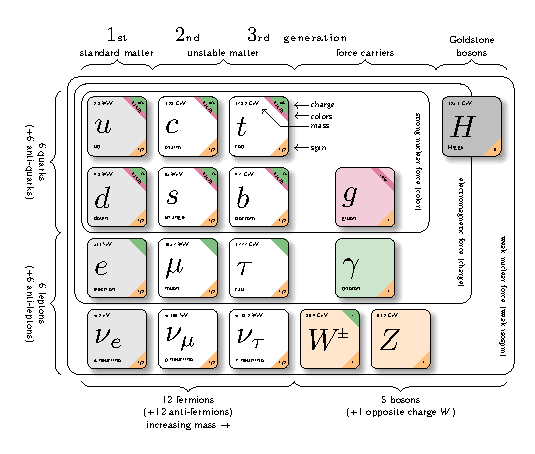
\includegraphics[width=0.83\textwidth]{ubonn-thesis/Chapters/Chapters_02/Figure/Standard_Model.pdf}
\caption{Standard Model of Particle Physics \cite{sm}}
\label{standardmodel}
\end{figure}

Each force operates on a different on a different range and with different strengths. The strong and weak forces are very limited range and dominate only on the level of subatomic interactions, while electromagnetic forces have infinite range. The SM consists of 17 fundamental particles classified into two groups: half-integer spin fermions, and integer spin bosons. The spin-1 (vector) bosons act as the mediators of interaction between particles and the spin-0 (scalar) Higgs boson acts as the mediator of Higgs interactions. An illustration of SM particles with their mass, charge and spin is presented in figure \ref{standardmodel}.



\subsection{Fermions}
There are 12 spin-$\frac{1}{2}$ fermions in the SM: 6 quarks and 6 leptons, which are grouped into 3 generations which are grouped into 3 generations. Each generation of quark contains one quark of charge +2/3e (up-type) and one quark of charge -1/3e (down-type). The quarks are (up-type followed by down-type): up (u) and down (d); charm (c) and strange (s); and top (t) and bottom (b). Similarly three lepton generations consists of electron (e), muon ($\mu$), and tau ($\tau$), and their corresponding neutrinos ($\nu_{e}$, $\nu_{\mu}$, $\nu_{\tau}$). The neutrinos have no electric charge, while the other leptons carry an electric charge of -1e. Each fermion has its corresponding anti-particle, with opposite sign on all charges (such as electric charge \& quantum numbers) but identical mass.

In the SM, a quark of one flavor can transform into a quark of another flavor via weak interaction. It strongly prefer to transform into another quark of its same generation. The transformation probability scale with the couplings in the Cabibbo-Kobayashi-Masakawa (CKM) matrix. For more details ref. \cite{Bargiotti:2000dn} can be referred.

\subsection{Bosons}

The remaining five particles in the SM are comprised of four vector type (spin-1) boson and one scalar type (spin-0) Higgs boson. Apart from the Higgs boson, all other bosons are called gauge bosons and are the mediators of the fundamental interactions between particles. Photons are the mediators of the electromagnetic force and are massless. The massive W and Z bosons   ($m_{W}$ = 80.379 GeV, $m_{Z}$ = 91.1876 GeV) are the mediators of the weak force while strong force is mediated by massless gluons. The gluons as well as quarks carry colour charge. There are three different colour charges: red, green, and blue. Additionally, there are also three anticolours (for antiparticles). Gluons themselves carry a combination of a colour and an anticolour charge and therefore they can couple to each other. There are only eight gluons in total because one of the nine colour combinations results in a non-existing colour singlet state. 

%\section{Physics at hadron colliders}

\section{Top quark physics}
The neutral Kaon decays experiment in 1964 by Christenson, Cronin, Fitch, and Turlay showed that weak interaction is not invariant under the combined discrete symmetry operation of charge conjugation C and parity P (CP violation) \cite{PhysRevLett.13.138}. Kobayashi and Maskawa realized that SM can provide a mechansim of CP violation through flavor mixing only if there are at least three generation of quarks \cite{kobayashi1973cp}. After the discovery of bottom quark in 1977 in Fermilab \cite{PhysRevLett.39.252}, the existence of the top quark as the weak isospin was expected. The top quark was first observed at the D0 and CDF collaborations on the Tevatron in $p\Bar{p}$ collisions in 1995 \cite{PhysRevLett.74.2626,PhysRevLett.74.2632}. Nowadays LHC is a top quark factory where top quarks are produced as discussed in section \ref{subsec:topquarkproduction}  .

\subsection{Top quark}
\label{subsec:topquark}
The top quark is the heaviest fundamental particle in the SM. It is up-type third generation quark. It has an electric charge Q = $\frac{2}{3}$, a mass of 173.3 $GeV/c^{2}$ and a decay width of $\Gamma_{t}(\alpha_{s}(M_{Z}) = 0.118)=$ 1.35 $GeV/c^{2}$ which corresponds to an average lifetime of $\tau_{t} \approx 0.5 \times 10^{-24}$ s \cite{ParticleDataGroup:2016lqr}. The top quark exclusively decays via weak interaction before hadronization, producing a W boson and a bottom quark because of its extremely short-lived lifetime. The absence of a hadron surrounding the top quark produces physicists with the unique opportunity to study the behaviour of a "bare" quark.

\subsection{Top quark production}
\label{subsec:topquarkproduction}

Top quarks are  dominantly produced in pairs through quark anti-quark annihilation and gluon-gluon fusion at leading order in QCD at haron colliders such as Tevatron and LHC. They are also produced singly through electroweak processes. At the LHC, top-quarks are mainly produced via gluon-gluon fusion. In this production mechanism two gluons from protons fuse into another gluon (see figures \ref{fig:gg1} and \ref{fig:gg2}) , or they exchange a virtual top quark and then emit a real $t\Bar{t}$ pair (see figure \ref{fig:vittt}). Figure \ref{fig:ttbarproduction} shows the leading order Feynman diagrams producing top anti-top pairs. 

\begin{figure}[h!] 
  \begin{subfigure}[b]{0.33\linewidth}
    \centering
    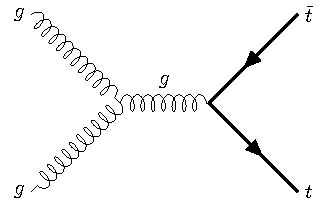
\includegraphics[width=\linewidth]{ubonn-thesis/Chapters/Chapters_02/Figure/ttbar_gluongluonchannel.pdf} 
  \caption{}
  \label{fig:gg1}
  \end{subfigure}%% 
  \begin{subfigure}[b]{0.33\linewidth}
    \centering
    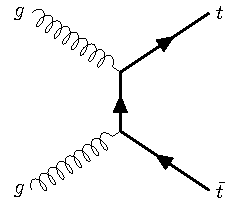
\includegraphics[width=0.76\linewidth]{ubonn-thesis/Chapters/Chapters_02/Figure/ttbar_Production_tchannel.pdf} 
  \caption{}
  \label{fig:gg2}
  \end{subfigure} 
  \begin{subfigure}[b]{0.33\linewidth}
    \centering
    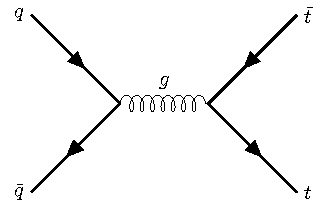
\includegraphics[width=\linewidth]{ubonn-thesis/Chapters/Chapters_02/Figure/ttbar_quarkquarkchannel.pdf} 
  \caption{}
  \label{fig:vittt}
  \end{subfigure}%%
  \caption{Leading order Feynman diagrams for $t\Bar{t}$ production via the strong interaction at the LHC}
  \label{fig:ttbarproduction}
  \end{figure}


Top quarks can also be produced singly in electroweak processes. The production processes are classified by the virtuality of the W boson exchanges in the process. The most abundant single top-quark production process at the LHC is t-channel production, followed by the associated production of a top quark and a real W boson, and s-channel production. Leading order diagrams of these processes are shown in figure \ref{fig:singletopproduction}. The production cross-section of these processes at LHC by the ATLAS colloboration is shown in figure \ref{ATLAS:singletop}. At the Tevatron, t-channel and s-channel single top-quark production are predicted by the SM, while Wt contribution is negligible \cite{singtop2014}.

\begin{figure}[h!] 
  \begin{subfigure}[b]{0.33\linewidth}
    \centering
    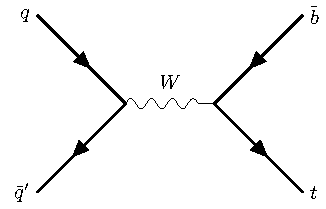
\includegraphics[width=0.96\linewidth]{ubonn-thesis/Chapters/Chapters_02/Figure/singletop_s-channel.pdf} 
  \caption{}
  \end{subfigure}%% 
  \begin{subfigure}[b]{0.33\linewidth}
    \centering
    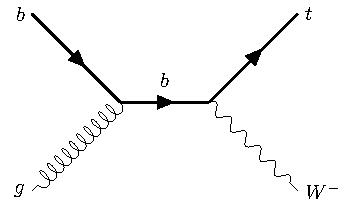
\includegraphics[width=\linewidth]{ubonn-thesis/Chapters/Chapters_02/Figure/singletop_realW.pdf} 
  \caption{}
  \end{subfigure} 
  \begin{subfigure}[b]{0.33\linewidth}
    \centering
    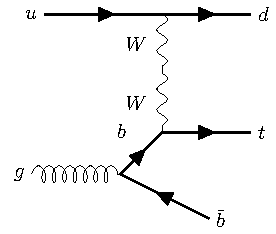
\includegraphics[width=0.76\linewidth]{ubonn-thesis/Chapters/Chapters_02/Figure/tchannel_4FS.pdf} 
  \caption{}
  \end{subfigure}%%
  \newline
  \centering
%  \vspace*{0.4cm}
  \begin{subfigure}[b]{0.4\linewidth}
    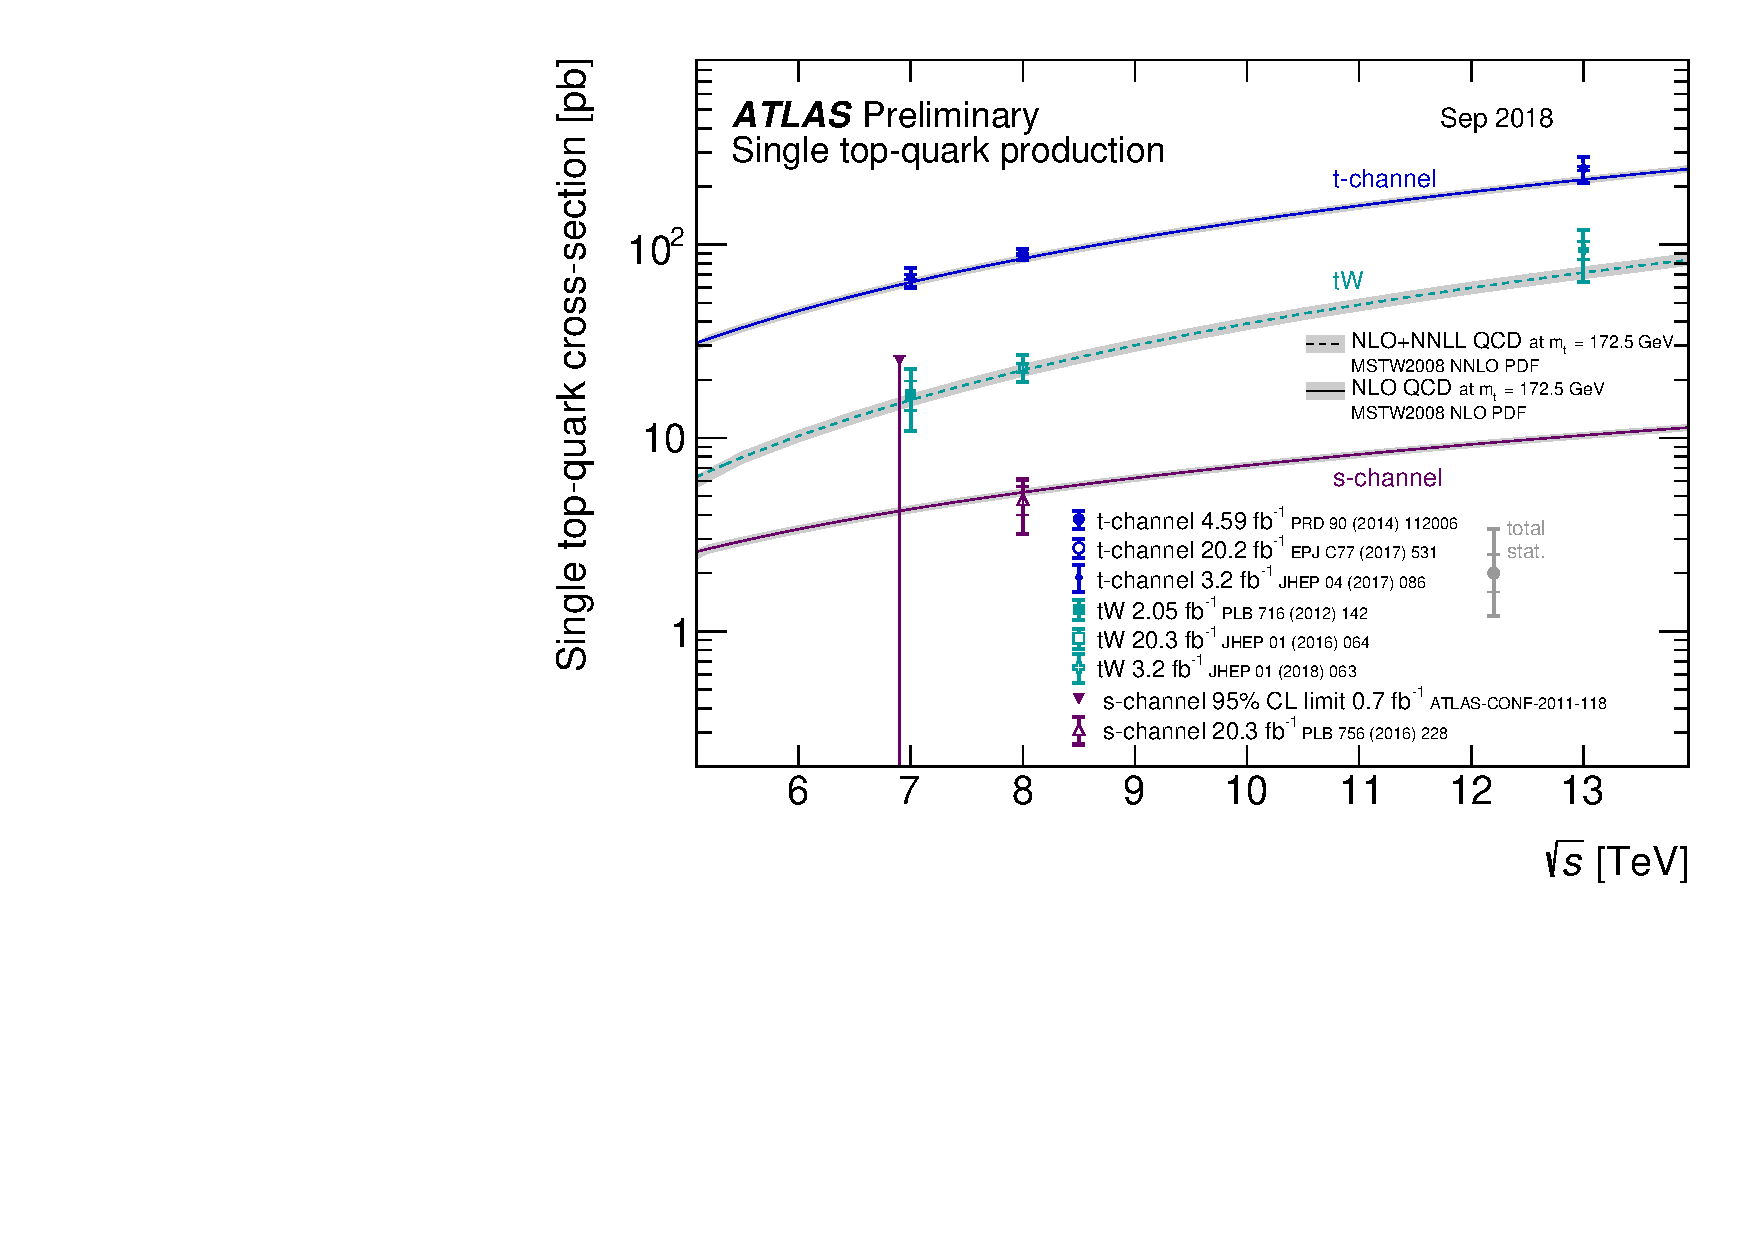
\includegraphics[width=\linewidth]{ubonn-thesis/Chapters/Chapters_02/Figure/singletop.pdf} 
  \caption{}
  \label{ATLAS:singletop}
  \end{subfigure}%%
  \caption{Feynman diagrams for single top quark production in the (a) s-channel, (b) in association with a W boson (c) t-channel production in 4FS , (d) measured single top quark production in ATLAS \cite{andrea}}
  \label{fig:singletopproduction}
  \end{figure}

By moving to next-to-leading order (NLO) electroweak production, there can be added to the single top processes, the radiation of a Z boson. This production process for which the total cross-section is measured in this thesis consists of a top quark, a forward-jet and a Z boson at the parton level. The top quark is produced via the t-channel and the Z boson is either radiated of from one of the participating quarks or produced via W boson fusion. The Feynman diagrams of the tZq process at the leading are shown in figure \ref{fig:tZQ}. As can be seen from figures \ref{topcoup} and \ref{wwzcoup}, tZq production offers access to the coupling of the top quark to a Z boson and additionally to the WWZ coupling. Measuring this process is therefore a very interesting test of the SM, since the production rate could be modified by several BSM theories (e.g. in vector-like quark models). 

\begin{figure}[h!] 
  \begin{subfigure}[b]{0.33\linewidth}
    \centering
    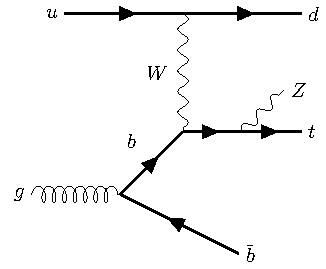
\includegraphics[width=0.7\linewidth]{ubonn-thesis/Chapters/Chapters_02/Figure/tZq_Zfromtop.pdf} 
  \caption{}
  \label{topcoup}
  \end{subfigure}%% 
  \begin{subfigure}[b]{0.33\linewidth}
    \centering
    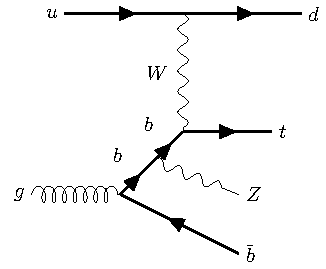
\includegraphics[width=0.7\linewidth]{ubonn-thesis/Chapters/Chapters_02/Figure/tZq_Zfromb.pdf} 
  \caption{}
  \end{subfigure} 
  \begin{subfigure}[b]{0.33\linewidth}
    \centering
    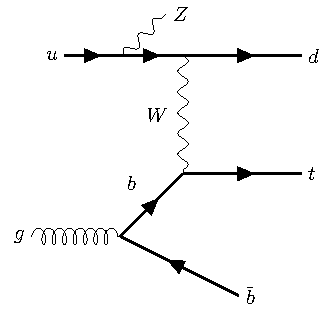
\includegraphics[width=0.7\linewidth]{ubonn-thesis/Chapters/Chapters_02/Figure/tZq_Zfromu.pdf} 
  \caption{}
  \end{subfigure}%%
  \newline
  \begin{subfigure}[b]{0.33\linewidth}
    \centering
    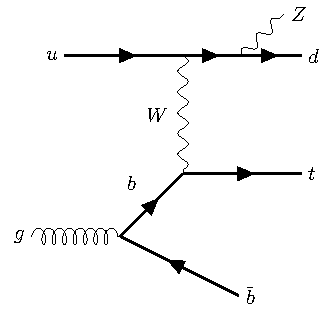
\includegraphics[width=0.7\linewidth]{ubonn-thesis/Chapters/Chapters_02/Figure/tZq_Zfromd.pdf} 
  \caption{}
  \end{subfigure}%% 
  \begin{subfigure}[b]{0.33\linewidth}
    \centering
    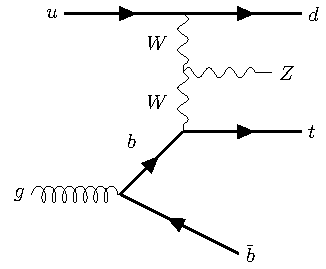
\includegraphics[width=0.7\linewidth]{ubonn-thesis/Chapters/Chapters_02/Figure/tZq_ZfromWW.pdf} 
  \caption{}
  \label{wwzcoup}
  \end{subfigure}
  \caption{Feynman graphs to calculate the lowest order amplitudes of the tZq process. In the four-flavour scheme, the b-quark originates from gluon splitting..}
  \label{fig:tZQ}
  \end{figure}

% !TEX root = mythesis.tex

%==============================================================================
\chapter{The LHC and the ATLAS experiment}
\label{chap:lhcandatlas}

In this chapter, the overall experimental setup is discussed. The Large Hadron Collider (LHC) which is the world's largest and the most powerful particle accelerator is discussed in section \ref{sec:largehadroncollider}. Furthermore, the main setup of the ATLAS detector, which is one of the two general-purpose detectors at the LHC is discussed in section \ref{sec:ATLAS}.

\section{The LHC}
\label{sec:largehadroncollider}

\begin{figure}[!h]
\centering
\includegraphics[width=0.7\textwidth]{ubonn-thesis/Chapters/Chapters_03/Figure/LHC.jpg}
\caption{The CERN Accelerator Complex and its pre-accelerator chain as well as the location of the four main experiments\cite{Haffner:1621894}. The LHC is the large blue ring, which is fed from its predecessor the Super Proton Synchrotron (SPS), shown in light blue, in turn fed from its own predecessor the Proton Synchrotron (PS), in magenta. }
%
\label{fig:LHC}
\end{figure}

The \textbf{L}arge \textbf{H}adron \textbf{C}ollider (LHC), located at the European Organization for Nuclear Research (CERN), is largest and most energetic particle collider ever constructed. It is currently operating at a record center-of-mass energy ($\sqrt{s}$) of 13 tera-electron-Volts (TeV) for proton-proton (pp) collisions. It allows scientists to reproduce the conditions that existed within a billionth of a second after the Big Bang by colliding beams of high-energy protons or ions at colossal speeds, close to the speed of light. Figure \ref{fig:LHC} gives an overview of the CERN accelerator complex. The LHC consists of a 27-kilometer ring of superconducting magnets with a number of accelerating structures to boost the energy of the particles along the way. Inside the accelerator, the particles are accelerated in opposite directions in two rings before they are made to collide. Before the particles are injected inside the beam pipes, they are injected into a linear accelerator (Linac 2) and are accelerated to an energy of 50 MeV. During this first acceleration, the protons are split into bunches. Then, they are injected into the Proton Synchroton Booster (PSB). From there, the protons are led to the Proton Synchroton (PS) with an energy of 1.4 GeV. Their energy is futher increased to 25 GeV, and they are then injected to the Super Proton Synchroton (SPS). Finally, the proton bunches pass to the LHC ring with an energy of 450 GeV, where they are accelerated to the desired energy. During Run I, the LHC operated at a center-of-mass energy of $\sqrt{s}$=7 TeV (2011) and at $\sqrt{s}$=8 TeV (2012). For Run II (2015-2018), the energy was increased to 13 TeV. The beams inside the LHC are made to collide at four locations around the accelerator ring, corresponding to the positions of four particle detectors ATLAS, CMS, ALICE and LHCb (see figure \ref{fig:LHC} ). The ATLAS and CMS detectors are cylindrically symmetrical multi-purpose detectors, which investigate a wide range of physics, from the search for the Higgs boson to extra dimensions and particles that could make up dark matter.

\section{The ATLAS detector}
\label{sec:ATLAS}


\begin{figure}[!h]
\centering
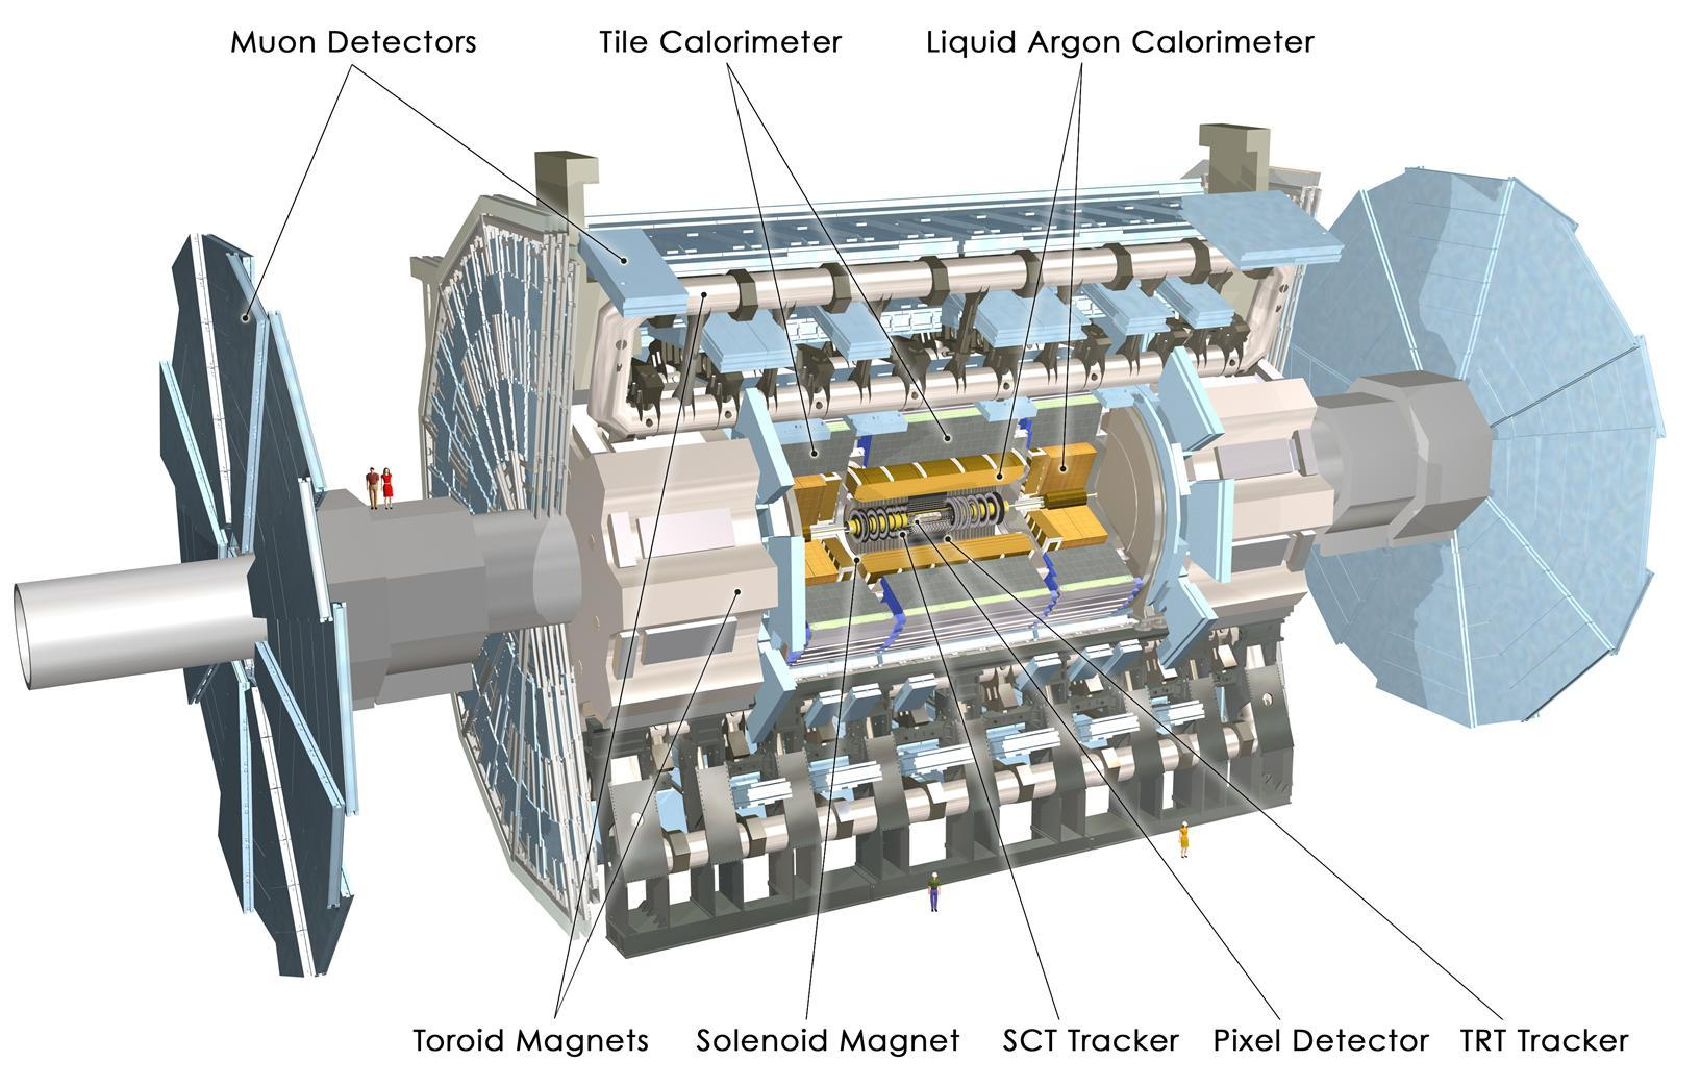
\includegraphics[width=0.6\textwidth]{ubonn-thesis/Chapters/Chapters_03/Figure/ATLAS_detector.pdf}
\caption{Overview over the entire ATLAS detector and its components \cite{PequenaoA}}
\label{fig:atlasdetector}
\end{figure}

The ATLAS detector (\textbf{A} \textbf{T}oroidal \textbf{L}HC \textbf{A}pparatu\textbf{S}) is one of the two largest particle detectors located at the LHC with a length of 44 meters, a diameter of 25 meters and 7000 tonnes of weight as shown in figure \ref{fig:atlasdetector}. It is the detector that is used to take the data for the analysis presented in this thesis and will also be assumed for the detector simulation of the Monte Carlo samples. The different detecting subsystems are arranged in layers around the collision point to record the paths, momentum, and energy of the particles, allowing them to be individually identified. It consists of three main detector components: the inner detector, the calorimeter system, and the muon spectrometer as shown in figure \ref{fig:atlasdetector} . Additionally, the inner detector contains several toroidal and solenoidal magnets whose purpose is to bend charged particles (see figure \ref{fig:atlasdetector} ). Charged particles such as leptons, charged mesons or charged hadrons can be detected through a combination of inner detector tracking and calorimeter deposits. Photons, neutral mesons or neural hadrons can be identified due to their deposits in calorimeter paired with missing curved tracking information from the inner detector. Neutrinos do not interact with the detector components and are inferred by summing all transverse momentum to determine a "missing" energy. A schematic diagram of different particles interacting with the detector components is shown in figure \ref{fig:particleinteraction}. 

\begin{figure}[!h]
\centering
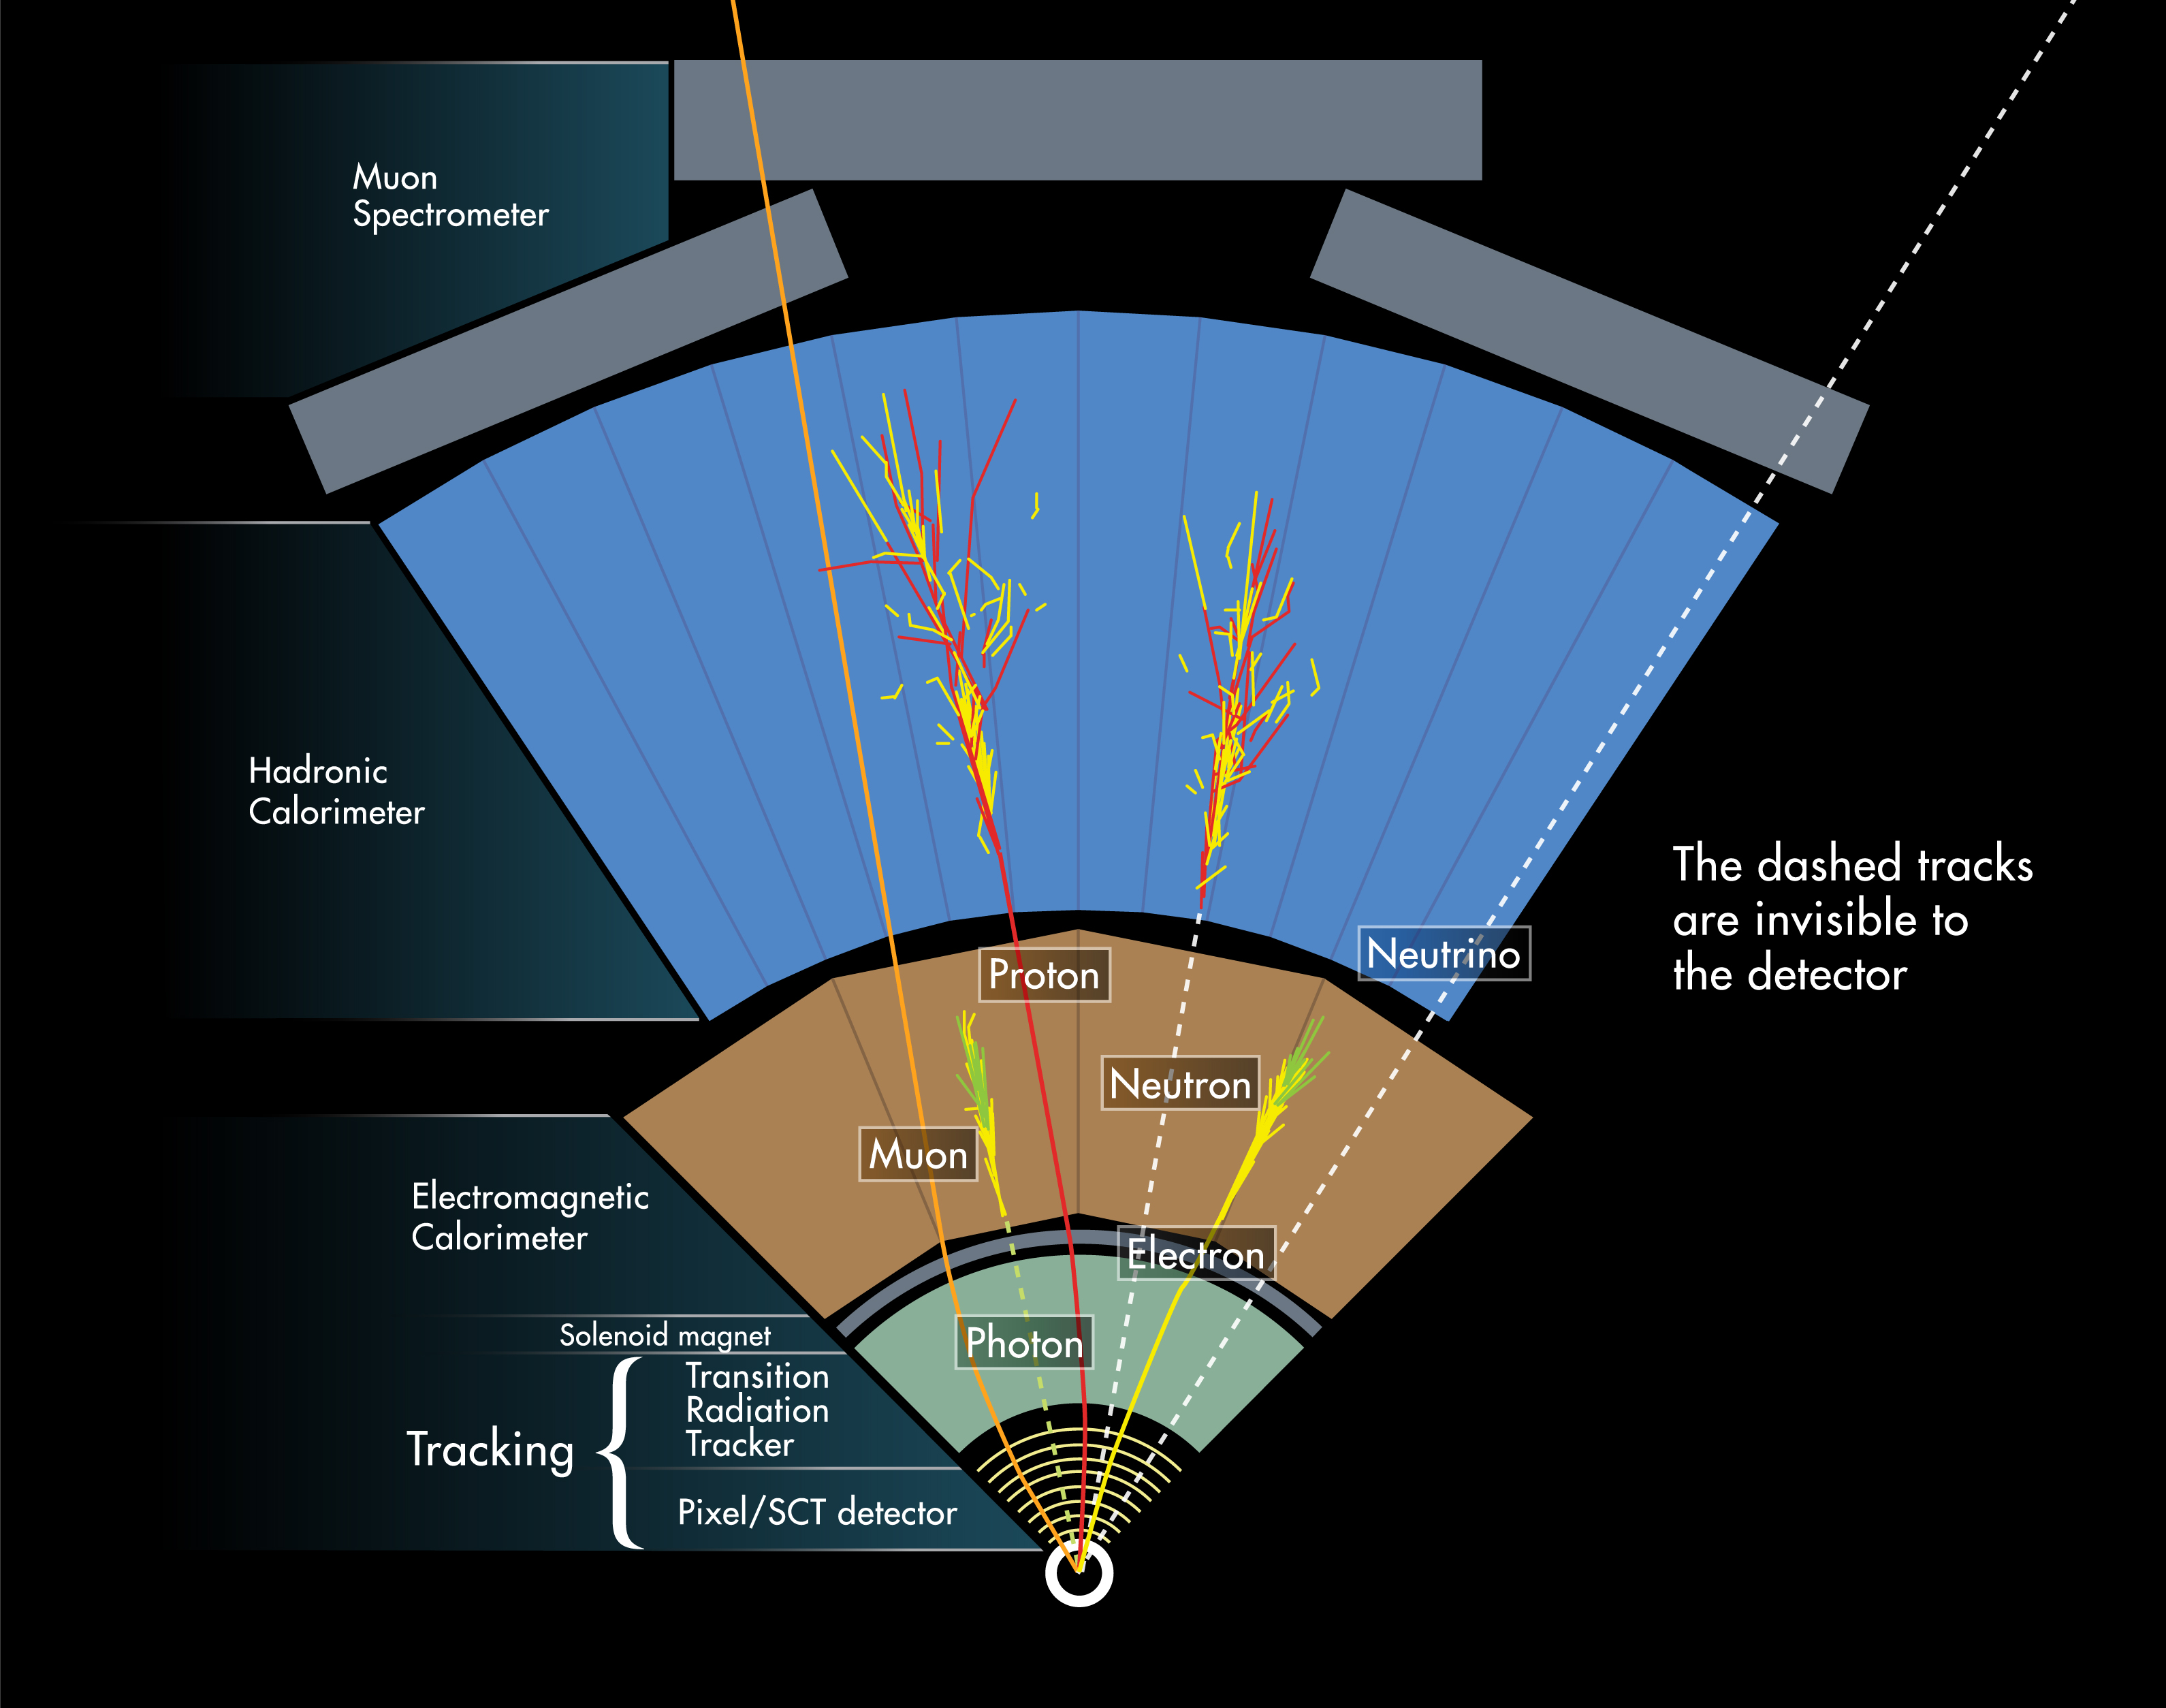
\includegraphics[width=0.6\textwidth]{ubonn-thesis/Chapters/Chapters_03/Figure/Particle_interaction.jpg}
\caption{ Depiction of the detectable particles upon a cross section of the ATLAS detector. \cite{PequenaoB}}
\label{fig:particleinteraction}
\end{figure}


\subsection{The ATLAS coordinate system}
\label{atlascoordinate}
ATLAS makes use of a right-handed coordinate system. The coordinate system has its origin at the nominal interaction point, with the z-axis pointed along the beamline. The x-y plane is transverse to the beam direction, with the positive x-axis pointing towards the center of the LHC ring and the positive y-axis defined as pointing upwards. Due to the symmetry, cylindrical coordinates are used, where $\phi$ is the angle along the plane transverse to the beam with respect to the x-axis and $\theta$ is the polar angle. Instead of the polar angle, pseudorapidity is used, which is defined as

\begin{equation}
    \label{pseudorapidity}
    \eta = - ln ( tan \frac{\theta}{2})
\end{equation}

The distance between two particles or objects in the $\eta$-$\phi$ plane is defined as
\begin{equation}
    \label{deltaR}
    \Delta R = \sqrt{(\Delta \eta)^{2} + (\Delta \phi)^{2}}
\end{equation}


\subsection{Inner detector}

\begin{figure}[!h]
\centering
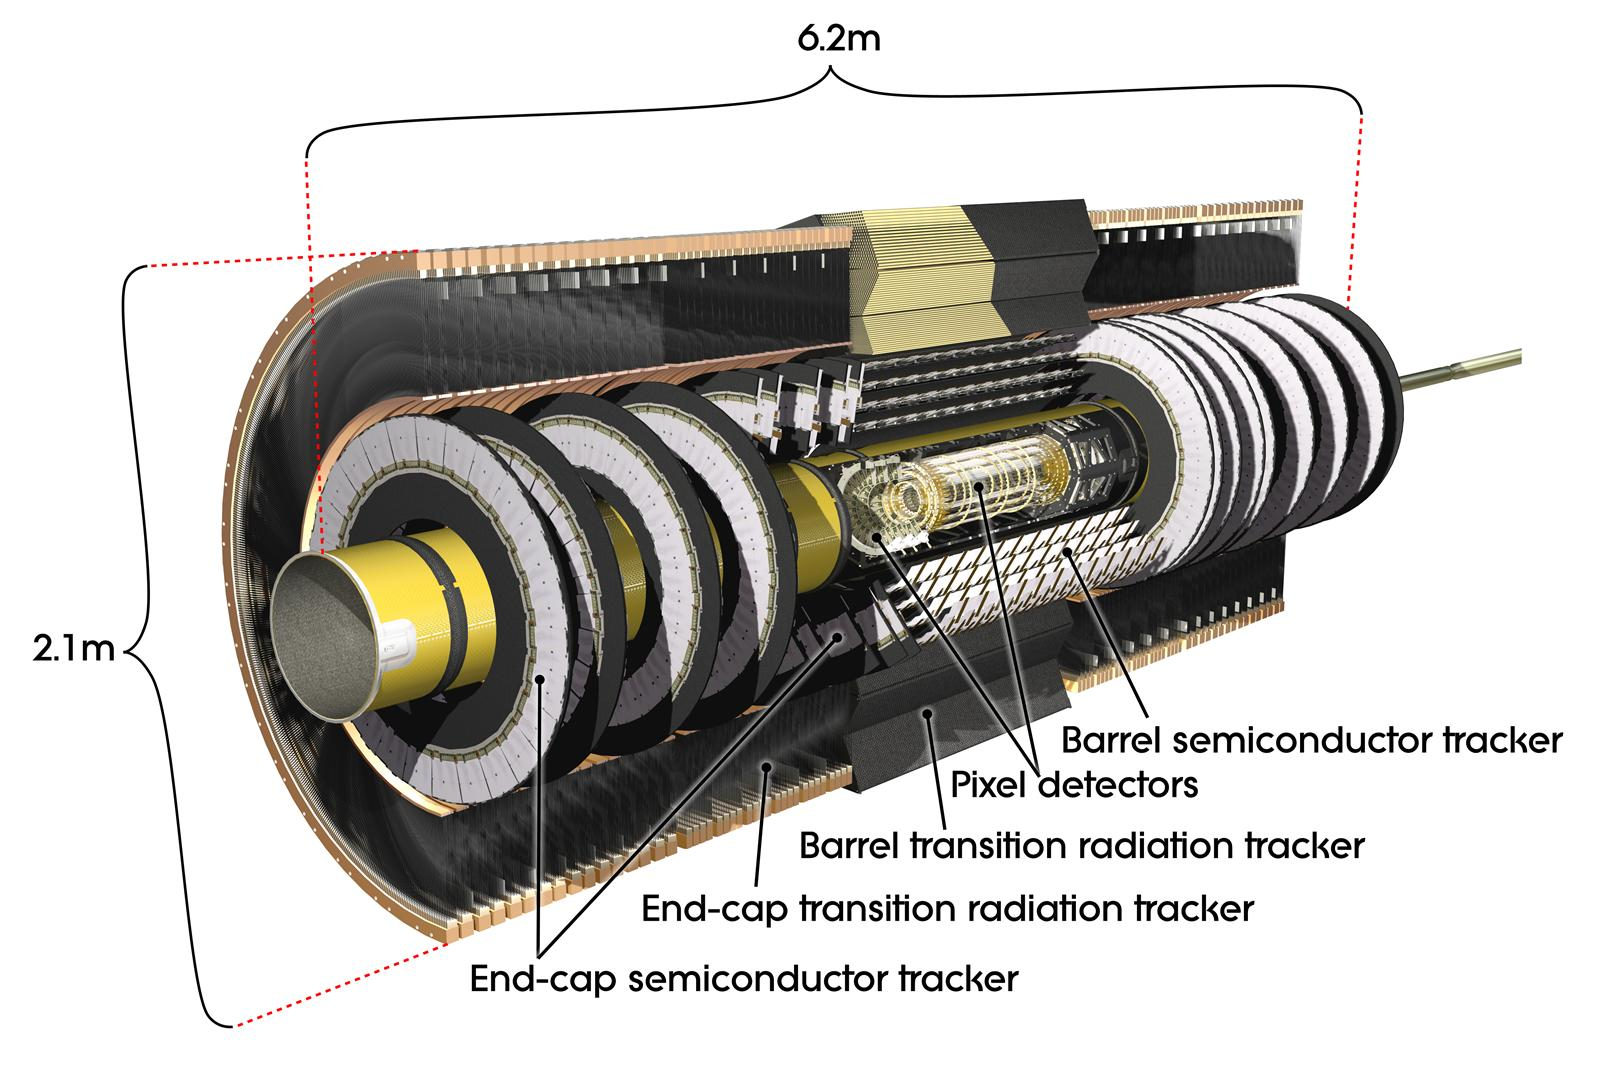
\includegraphics[width=0.6\textwidth]{ubonn-thesis/Chapters/Chapters_03/Figure/inner_detector.jpg}
\caption{ Cut-away view of the ATLAS inner detector \cite{Pequenao:1095926}}
\label{fig:atlasinnerdetector}
\end{figure}

The inner detector is the compact and highly sensitive part of the ATLAS detector that is used to measure the direction, momentum, and charge of electrically-charged particles produced in each proton-proton collision. It consists of three different systems of sensors, all immersed in a magnetic field of 2 T produced by a solenoid located between the tracking system and the calorimeter, parallel to the beam axis. The magnetic field bends the tracks of charged particles allowing a measurement of their momentum. The main components of the inner detector are Pixel Detector, Semiconductor Tracker (SCT), and Transition Radiation Tracker (TRT) as shown in figure \ref{fig:atlasinnerdetector}. 

The pixel detector is the inner part of the detector which is divided into barrel part and an end-cap region covering the range of $|\eta|$<2.5. The barrel region starts 5 cm away from the interaction point making it the detector subsystem closest to the beam pipe. There are four barrel layers with 1736 sensor modules. In the end-cap region, each site constitutes three detector discs oriented perpendicular to the beam pipe with 288 modules. The individual module consists of pixels with size of 50\times400 $\mu m^{2}$ in the external layers and 50\times250 $\mu m^{2}$ in the innermost layers. Thus, the pixel detector plays an important role in the reconstruction of primary and secondary vertices, the latter being useful information for b-tagging.

SCT consists of stereo silicon strips forming four concentic cylinders and nine end-cap discs on each side. It consists of a total of almost 16000 strip sensors, each 6.4 cm long and having an 80 $\mu m$ pitch. It helps in simultaneous measurement of R and $\phi$. TRT is the outer-most part of the inner detector that helps in precision measurement and provides an additional information on the particle type (pions or electrons) that flew through the detector. It consists of thin straw tubes with a diameter of 4 mm, which contain a 0.03 mm thin gold-plated tungsten wire in the centre. They are filled with a gas mixture of Xe, CO$_{2}$, and O$_{2}$.

\subsection{Calorimetry}
\label{sec:calorimetry}

\begin{figure}[!h]
\centering
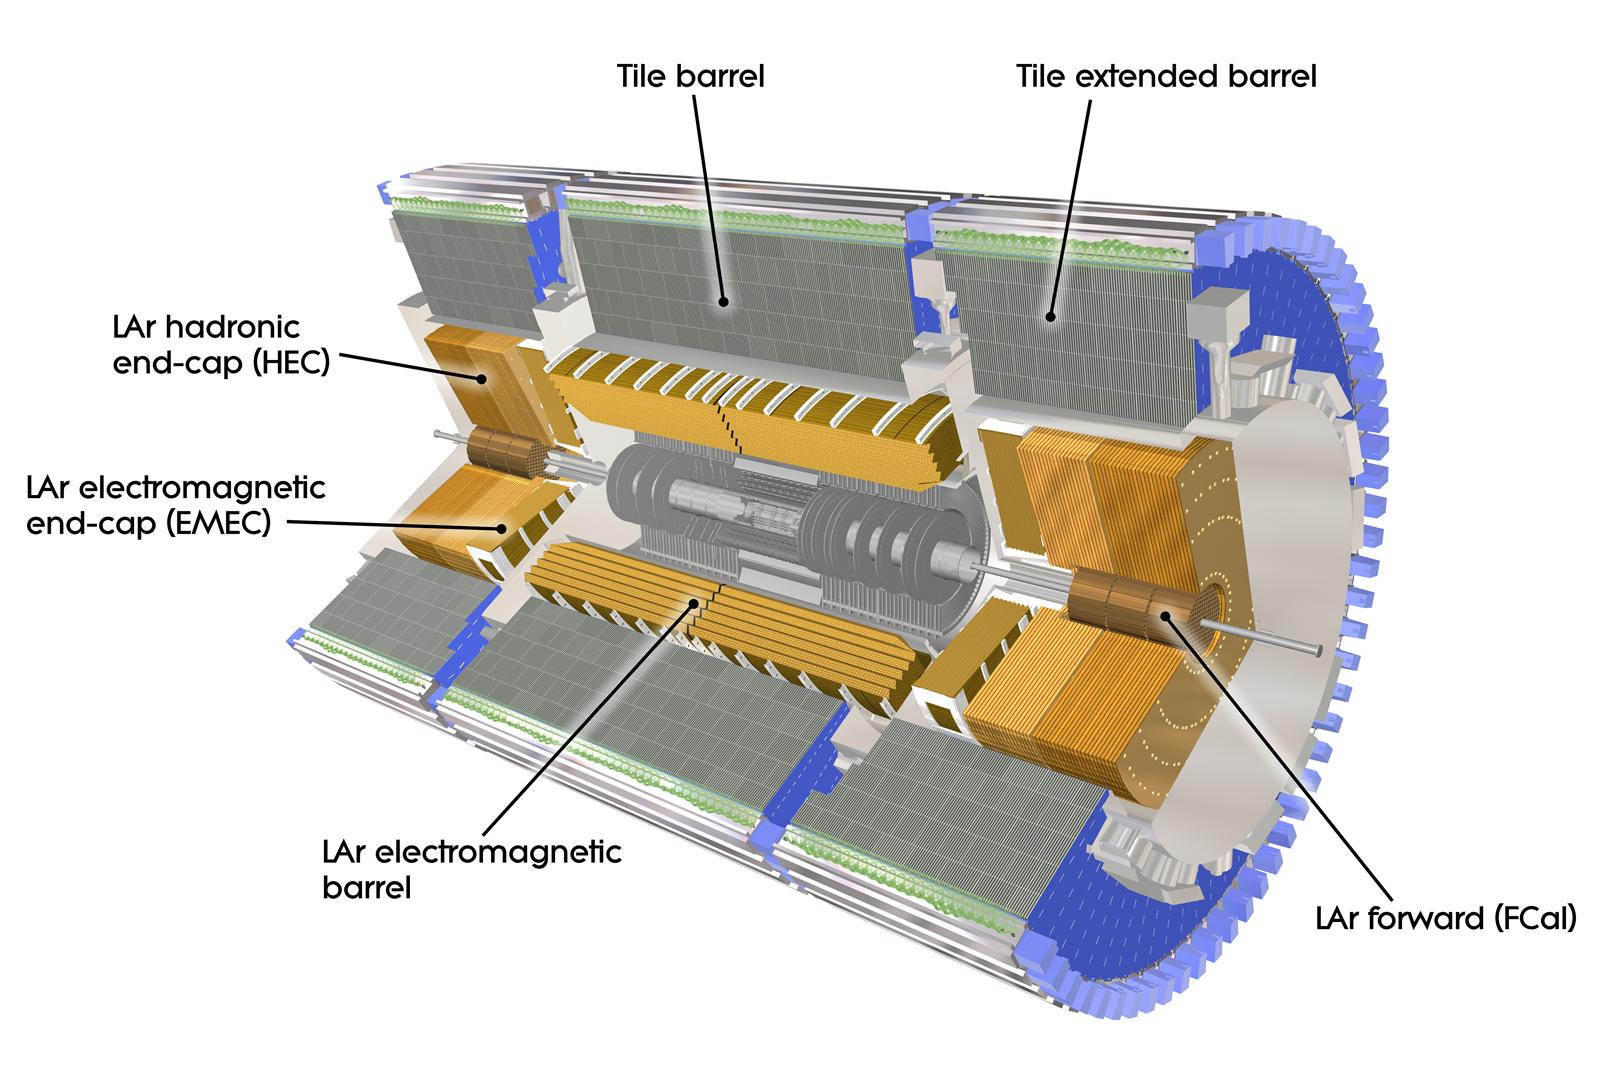
\includegraphics[width=0.6\textwidth]{ubonn-thesis/Chapters/Chapters_03/Figure/calorimeter.jpg}
\caption{Cut-away view of the ATLAS calorimeter \cite{Pequenao:1095927}.}
\label{fig:calorimeter}
\end{figure}


The calorimeter system of the ATLAS detector is divided into 2 subsystems, the inner electromagnetic calorimeter (EMcal) and the outer hadronic calorimeter (Hcal). Both the calorimeters are composed of multiple layers, alternating between an absorber material, which induces particle reactions leading to so called showers and an easy ionizable active material to detect the particles emerging from the absorber material. An overview of the ATLAS calorimeter is shown in figure \ref{fig:calorimeter} . 

EMcal measures the deposited energy of electrons and photons. It is divided into a barrel part and two end-caps. Lead is used as absorber material while liquid argon (LAr) is used as active medium. A combined tile calorimeter and two sample calorimeters in the end-cap regions are used as Hcal. Hcal measures the deposited energy of hadrons. Here, copper is used as active material and LAr as active material. The energy resolution of the calorimeter system can be parametrised as

\begin{equation}
    \label{calorimeter}
     \frac{\sigma(E)}{E} = \frac{a}{\sqrt{E(GeV)}}\oplus b
\end{equation}

For the electromagnetic calorimeter, the corresponding parameters are the stochastic term a $\approx$ 10\% and the constant b $\approx$ 0.7\%, reflecting local non-uniformities in the calorimeter response. For the hadronic calorimeter, the parameters are a $\approx$ 50\% and b $\approx$ 3\% in the barrel and end-cap parts.

\subsection{Muon system}
\label{sec:muonsystem}
Muons are the only SM particles besides neutrinos that escape the inner detector and calorimeters. Muon spectrometer is the outermost layer of the ATLAS detector. It detects muons and measures the properties of their tracks bent in the torodial magnetic field, using high-precision tracking chambers. It is made up of 4,000 individual muon chambers.  It measures the paths of the muons that pass through over a total area the size of a footbal field, to an accuracy of less than one-hundredth of a millimeter. The muon spectrometer is also responsible for the enormous size of the ATLAS detector.





\subsection{Trigger system}
\label{sec:triggersystem}

The ATLAS trigger system selects data in a way that the event at hand contains physics process of interest for the analysis. It consists of the hardware-based level-1 trigger (L1) and the software-based high-level trigger (HLT). Starting with a rate of proton-proton collision events of approximately 40 MHz is reduced to nearly 1 kHz after passing the event filter. The L1 uses a small amount of information from the calorimeters and muon spectrometer to looks for objects and subsequently, regions of interest are built. The HLT is able to access full event data and analyses the regions of interest defined by the L1. After deciding whether to keep the event or not, the events are recorded for physics analysis after passing the event filter.  

\section{Physics objects reconstruction in ATLAS}

In this section, the physics objects that are presented in this thesis is discussed. Electrons, muons, jets, bjets and missing transverse momentum are considered as physics objects. Their definitions are as follow

\subsection{Electrons}
\label{subsec:electron}

Electron candidates are identified using a likelihood-based multivariate method which takes information about the energy deposit in the electromagnetic calorimeter and inner detector tracks. The energy deposit clusters are required to have transverse energy $E_{T}>$ 15 GeV and be found in the pseudorapidity range $|\eta|<$ 2.7 region, excluding the transition region between the barrel and end-cap EMcal found between 1.37 $<|\eta|<$ 1.52. The transverse impact parameter has to fulfill $|d_{0}/\sigma(d_{0})|<$ 5 and $|z_{0}sin(\theta)|<$ 0.5 mm. Here $d_{0}$ and $z_{0}$ refer to the transverse and longitudinal distance of closest approach between the track and the primary vertex. Three quality requirements are available, in order of increasing background rejection power: LooseLH, MediumLH and TightLH. For this analysis all electron candidates are required to pass the TightLH working point. Beyond the quality cut, electrons are required to be isolated using working point discussed in section \ref{subsec:LWP}

\subsection{Muons}
\label{subsec:muons}
Muons are identified by the reconstruction of tracks in the inner detector and the muon spectrometer. To increase background rejection, some additional requirements are placed placed on track-parameter quality in the order of increasing background rejection power: Loose, Medium and Tight. They also have to fulfil $|d_{0}/\sigma(d_{0})|<$ 3 and $|z_{0}sin(\theta)|<$ 0.5 mm. Muon candidates for this analysis pass the Medium identification working point.


\subsection{Jets}
Jets which represent cascades of matter generated in the process of quark hadronization are reconstructed from topological calorimeter clusters using the anti-k$_{t}$ algorithm with a radius parameter of 0.4. They are required to have $P_{T}>$ 35 GeV and $|\eta|<$ 4.5. To suppress jets from pile-up, the Jet Vertex Tagger (JVT) is used.

\subsection{b-jets}
Identifying b-jets, which are jets from hadrons containing bottom quarks, is crucial for analyses with top quarks, since the top quark decays in almost 100\% of all cases into a W boson and a bottom quark. b-jets are identified with the DL1r algorithm. Specially DL1r$\_$PC variant is used; corresping to the current recommendation. The chosen working point is 70\% due to the optimal signal to background ratio.

\subsection{Missing transverse energy}
Missing transverse momentum $E_{T}^{miss}$ is defined as the magnitude of the transverse momentum vector which quantifies the transverse momentum imbalance of all detectable momenta. Since neutrinos will pass the ATLAS detector without interacting with any of its sub-detectors, events containing neutrinos will contain $E_{T}^{miss}$ due to energy-momentum conservation. The $E_{T}^{miss}$ is calculated as the magnitude of the negative sum of the transverse momenta of all identified jets, electrons and muons in the event, as well as soft term built from tracks that are associated to the hard-scatter vertex but are not associated to any of the reconstructed objects. 


% !TEX root = mythesis.tex

%==============================================================================
\chapter{Data and Monte Carlo simulated events}
\label{chap:data_MC}
%==============================================================================
\section{Data sample}
\label{sec:data_sample}

The analysis presented in this thesis uses data collected from 2015 to 2018 by the ATLAS detector at a center-of-mass energy of 13 TeV, The selected data periods were collected during stable beam LHC operations and with the ATLAS detector fully functioning. The total integrated luminosity is 139 fb$^{-1}$. Figure \ref{atlasluminosity} shows the total integrated luminosity over time. The considered data events have been recorded by either electron or muon trigger. There were later filtered using so-called the Good Run List (GRL), which requires that the LHC beam has conditions to qualify it for physics analysis and is is shown in blue in figure \ref{atlasluminosity}.

\begin{figure}[!h]
\centering
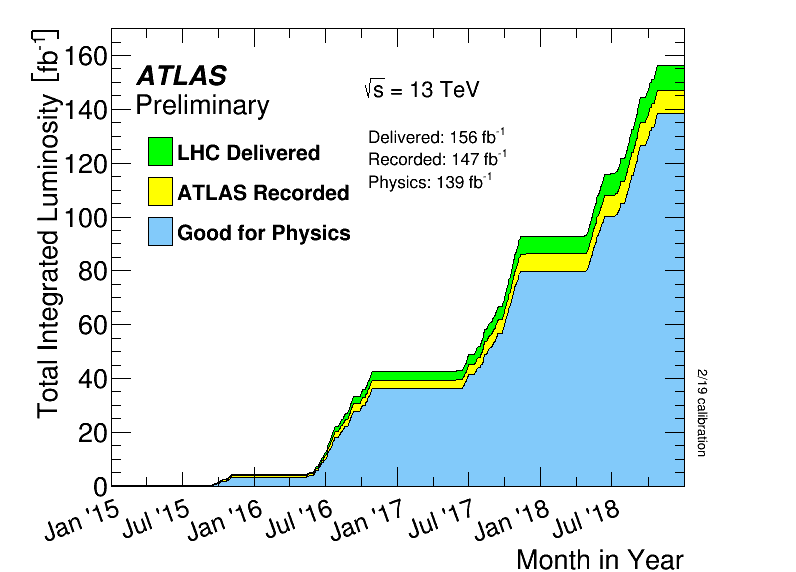
\includegraphics[width=0.7\textwidth]{ubonn-thesis/Chapters/Chapters_04/Figure/intlumivstimeRun2DQall.png}
\caption{Cumulative luminosity versus time delivered to ATLAS (green), recorded by ATLAS (yellow), and certified to be good quality data (blue) during stable beams for pp collisions at 13 TeV centre-of-mass energy in 2015-2018 \cite{ATLAS-CONF-2020-023}}
\label{atlasluminosity}
\end{figure}


\section{Monte Carlo simulation}
\label{sec:MC}
Monte-Carlo (MC) simulation is an inevitable component of the ATLAS experiment in order to simulate all physics processes considered in the analysis. Because MC events are used to validate the analysis procedures to calculate the acceptance for the signal channel and to evaluate the contributions from the background processes. The MC simulation is divided into three steps \cite{buckley2019monte}: The first is the detector independent generation of collision events which can be done by various extenal MC event generators interfaced by the ATLAS software framework Athena \cite{atlas_collaboration_2019_2641997} . The event generation of the MC simulation includes the parton shower and hadronization process. The nect step of the MC simulation is the detector simulation, where a realistic picture of the energy deposit in the sensitive parts of the detector is simulated. The GEANT4 \cite{GEANT4:2002zbu} toolkit is used to perform this simulation. It relies on the detector geometry, which describe physics constructions and conditions (e.g. magnetic field, alignment of detectors parts, dead read-out channels) of the detector. The last step of the MC simulation of all events is the digitization of the simulation hits. At this step, the energy deposited inside the sensitive part of the detector is translated to an increase of a voltage or an electric current in a given read-out channel with further digitization of this analog electronic signal. The output of digitization is recorded in so-called digits. Digits are inputs for further emulation of the detector read-out electronics, Read Out Drives (ROD); which produce the so called Rae Data Objects (RDO). RDOs are the inputs for the offline reconstruction of physical objects. After the digitization step, the MC simulated events and data are equivalently treated by the event reconstruction algorithms. 

All the above described major steps of the MC simulation are brought together in the simulation software of the Athena framework. Further processing of the simulated events implies reconstruction for the physics results. 


\subsection{Signal sample}
\label{subsec:Sig}
The tZq sample is simulated using the MadGraph5$\_$aMC@NLOv2.3.3 \cite{madgraph2014} generator at NLO with NNPDF3.ONO parton distribution function (PDF). The four flavor scheme is used where all the quark masses are set to zero, except for the top and bottom quarks. The SM tl$^{+}$l$^{-}$q MC sample used in the analysis (DSID:412063) contains a trilepton filter. The top quark decays as expected in the SM, t$\rightarrow$bW. Only the leptonic decay of the W boson is considered.  


\subsection{Background sample}
\label{subsec:bkg}

Several SM processes are expected to have the same final-state particles as the signal events and are considered as a background to the tZq trilepton analysis. The event signature which has been searched consists of a high $p_{T}$ b-quark, three-charged leptons ($\mu$, e) and missing transverse energy ($\cancel{E}_{T}$), from the neutrino of the semi-leptonic W boson decays. The main backgrounds are therefore WZ, ZZ, $t\Bar{t}$, Z+jets, $t\Bar{t}Z$, tWZ etc.  The background processes WZ shown in figure \ref{WZ}, ZZ in figure \ref{ZZ}, tWZ in figure \ref{tWZ}, $t\Bar{t}Z$ figure \ref{ttZ}, have three real leptons in the final state. Whereas background processes such as Z+jets shown in figure \ref{Z+jets}, $t\Bar{t}$ in figure \ref{ttbar}, and tW have only two real leptons in the final state. The third lepton can come from the semi-leptonic b-jets or mis-identification of other object quantities. These backgrounds with non-prompt leptons are called fake backgrounds.

\begin{figure}[!h] 
  \begin{subfigure}[b]{0.3\linewidth}
    \centering
    \hspace*{-0.9cm}
    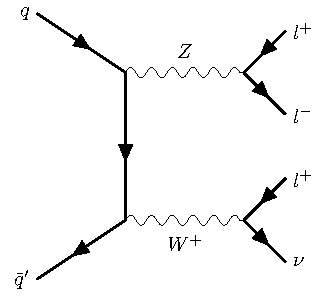
\includegraphics[width=\textwidth]{ubonn-thesis/Chapters/Chapters_04/Figure/Feynman_WZ.pdf}
    \caption{}
    \label{WZ}
  \end{subfigure}%% 
  \begin{subfigure}[b]{0.3\linewidth}
    \centering
    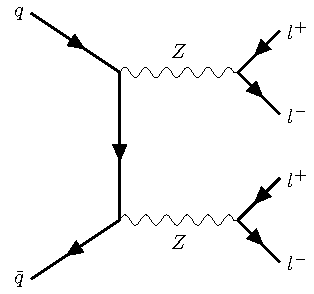
\includegraphics[width=\textwidth]{ubonn-thesis/Chapters/Chapters_04/Figure/Feynman_ZZ.pdf} 
    \caption{}
    \label{ZZ}
  \end{subfigure} 
  \begin{subfigure}[b]{0.3\linewidth}
    \centering
    \vspace*{-2.8cm}
    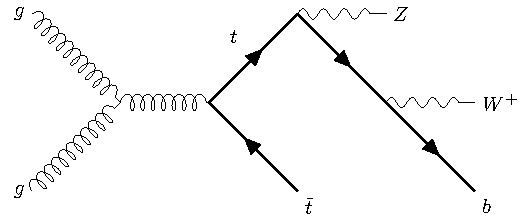
\includegraphics[width=\textwidth]{ubonn-thesis/Chapters/Chapters_04/Figure/tWZ_Feynman.pdf} 
    \caption{}
    \label{tWZ}
  \end{subfigure}%%
  \newline
  \begin{subfigure}[b]{0.3\linewidth}
    \centering
    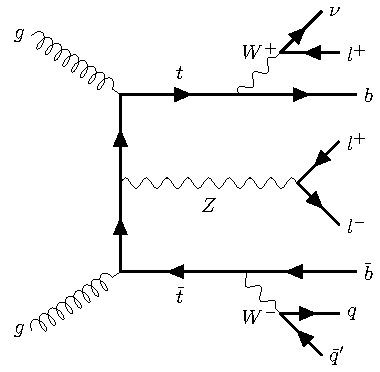
\includegraphics[width=0.9\textwidth]{ubonn-thesis/Chapters/Chapters_04/Figure/Feynman_ttbarV.pdf} 
    \caption{}
    \label{ttZ}
  \end{subfigure} 
  \begin{subfigure}[b]{0.3\linewidth}
    \centering
    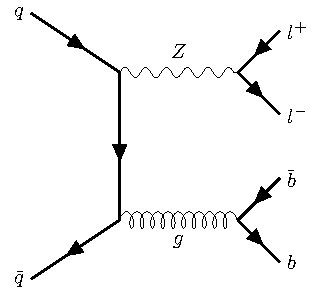
\includegraphics[width=0.9\textwidth]{ubonn-thesis/Chapters/Chapters_04/Figure/ZPlusJets_standalone.pdf} 
    \caption{}
    \label{Z+jets}
  \end{subfigure} 
  \begin{subfigure}[b]{0.3\linewidth}
    \centering
    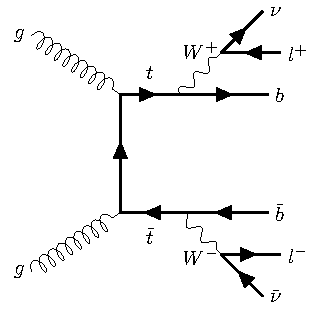
\includegraphics[width=0.9\textwidth]{ubonn-thesis/Chapters/Chapters_04/Figure/ttbar_standalone.pdf} 
    \caption{}
    \label{ttbar}
  \end{subfigure} 
  \caption{The leading order Feynman diagrams of the dominant background processes. (a) Diboson (WZ), (b) Diboson (ZZ), (c) tWZ, (d) $t\Bar{t}Z$, (e) Z+jets, and (f) $t\Bar{t}$}
  \label{background_feynman}
\end{figure}


Details of all simulated samples are given in table \ref{tab:backgrounds}.

\begin{table}[!h]
     \centering
      \begin{tabular}{@{} *6l  @{}}
      \toprule
      Process & MC generator & Parton shower & PDF set \\
     \midrule
      WZ & SHERPA 2.2.2 \cite{sherpa12004,sherpa2009} & SHERPA  & NNPDF3.0NNLO  \\[0.2ex] 
      ZZ & SHERPA 2.2.2 & SHERPA & NNPDF3.0NNLO  \\[0.2ex]
      $t\Bar{t}$ & POWHEG \cite{powhegOleari:2010nx} & Pythia 8 \cite{pythia2006} & NNPDF2.3LO  \\[0.2ex]
      tW & POWHEG & Pythia 8 & NNPDF2.3LO  \\[0.2ex]
      Z+jets & SHERPA 2.2.1 & SHERPA & NNPDF3.0NNLO  \\[0.2ex]
      $t\Bar{t}V$ & MadGraph5$\_$aMC@NLO & Pythia 8 \cite{pythia82015}&  NNPDF2.3LO  \\[0.2ex]
      tWZ & MadGraph5$\_$aMC@NLO & Pythia 8 &  NNPDF2.3LO  \\[0.2ex]
      $t\Bar{t}H$ & POWHEG  & Pythia 8 &  NNPDF2.3LO  \\[0.2ex]
      \bottomrule
 \end{tabular}
 \caption{Overview of background MC generated samples.}
 \label{tab:backgrounds}
 \end{table}

\newpage

\subsection{Reweighting of Monte-Carlo simulated events}
\label{subsec:reweightingofMC}
The number of events generated during the MC simulations generally do not exactly match the number of expected events for a given physical process at a given integrated luminosity. Each MC event is given a weight to rescale it so that the overall MC sample accurately represents the physical processes. Thus, to correctly reproduce the data-taking conditions, as well as replicate the efficiency of selecting different physics objects, in the simulated samples, event-by-event correction factors are applied to the MC events. The total event weight can be written as:
\begin{equation}
    \label{eqn:weight}
    w_{event} = w_{MC}\times w_{pile-up} \times w_{lepton} \times w_{JVT} \times w_{trigger} \times w_{b-tagging}
\end{equation}

The term $ w_{MC}$ is the MC event weight. The $ w_{pile-up}$ term is introduced to the MC samples, as a certain pile-up profile is assumed during MC simulation where as  $ w_{lepton}$ term is related to the efficiency of reconstructing, identifying a certain lepton. The $ w_{trigger}$ term is realted to the trigger. The final state considered for analysis consists of a  b-tagged jet, thus   $ w_{b-tagging}$ weight is applied.

\subsection{Luminosity reweighting}
\label{subsec:luminosityreweighting}

\begin{figure}[!h]
\centering
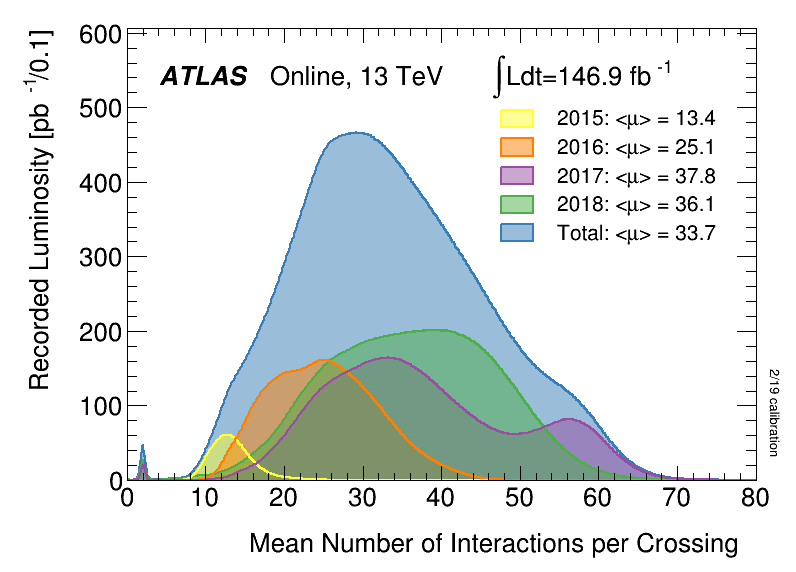
\includegraphics[width=0.5\textwidth]{ubonn-thesis/Chapters/Chapters_04/Figure/mu_2015_2018.png}
\caption{Luminosity weighted plot of the mean number of interactions per crossing for the 2015 and 2016 datasets \cite{ATLAS-CONF-2020-023}.}
\label{}
\end{figure}


The signal and background processes are simulated with large statistics. Thus, the luminosity for the MC simulated samples are very high. In order to correctly match the process to a dataset, the luminosity of the MC sample is scaled. The weight or scale factor is defined as 

\begin{equation}
    \label{luminosity}
    w_{lumi} = \frac{\sigma_{process}}{N} \mathcal{L}
\end{equation}

$\sigma_{process}$ is the cross-section of the specific physical process. $\mathcal{L}$ is the integrated luminosity of the data sample and N is the number of events in the original MC sample.


% !TEX root = mythesis.tex

%==============================================================================
\chapter{Events selection}
\label{chap:event_selection}

The goal of the event selection is to achieve the highest possible fraction of tZq events in data as predicted by Monte Carlo simulation. Data events are selected if they pass the pre-selection criteria discussed in section \ref{sec:data_sample}. The pre-selection treatments are also applied on MC events. In order to verify the modeling of physics processes in the relevant areas of kinematic phase space, a set of signal, and control regions are defined. Each region is defined by a set of selection cuts on the reconstructed variables. These reconstructed variables can also be the one from intermediate-state particles which are calculated from the final state observables. 
%==============================================================================

\section{Signal region}
\label{sec:SR}

As shown in the Feynman diagrams in figure \ref{fig:tZQ}, the tZq signal consists of a top quark, a forward-jet and a Z boson. The final state at the leading order for which the analysis is performed consists of three leptons, one neutrino, one b-quark and a light quark which is expected in the forward direction.  The two of the three leptons come form the Z decay and the one from the leptonic W decay. 

\begin{figure}[h!] 
  \begin{subfigure}[b]{0.48\linewidth}
    \centering
    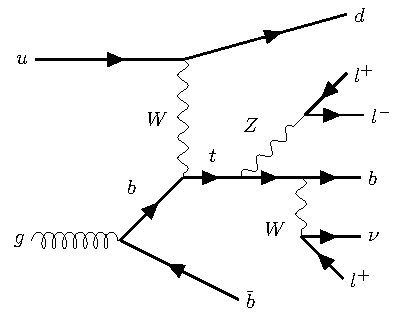
\includegraphics[width=0.7\linewidth]{ubonn-thesis/Chapters/Chapters_05/Figure/tZq_Zfromtop_decay.pdf} 
  \caption{}
  \label{fig:tZq-Zdecay}
  \end{subfigure}%% 
  \begin{subfigure}[b]{0.48\linewidth}
    \centering
    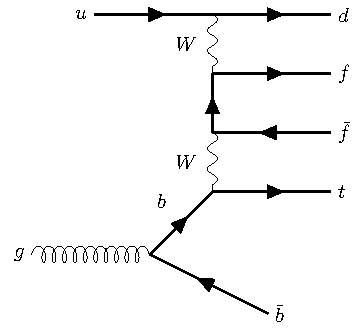
\includegraphics[width=0.7\linewidth]{ubonn-thesis/Chapters/Chapters_05/Figure/tZq_NoZ.pdf} 
  \caption{}
  \label{fig:tZq-nonZdecay}
  \end{subfigure} 
  \caption{Leading order Feynman diagrams with the trilepton final state. (a) resonant production of dilepton pairs, (b) non-resonant production of dilepon pairs }
  \label{fig:tZqdecay}
  \end{figure}


The Feynman diagrams for the trilepton final state at the leading order is shown in figure \ref{fig:tZqdecay}. The signal has also contributions from the non-resonant dilepton production as in figure \ref{fig:tZq-nonZdecay}. The QCD calculations at NLO suggests that there can exist significant QCD radiation present in the event which can manifest itself in the form of a third reconstructed jet. 

In order to increase acceptance as much as reasonably possible two orthogonal signal regions (SRs) named as SR 2j1b and SR 3j1b are defined. In SR 2j1b, events with three leptons, one b-tagged jet and one untagged jet as forward jet are selected. In SR 3j1b, events are selected identically to the SR-2j1b except for the inclusion of a second untagged jet. One of the two untagged jets, that one that gives, with the b-jet, the highest invariant mass, $m_{bj_{f}}$ is selected to be the forward jet. The remaining jet is called radiation jet. The same nomenclature is used for the jets in the control regions (CRs)

\subsection{Full event reconstruction}
\label{sec:event_reconstruction}

From the final states of the process, the variables are reconstructed. The reconstructed variables are the one directly measured in the detector or the intermediate one, calculated from the final state observables.  In order to reconstruct the Z boson, an opposite-sign, same-flavor (OSSF) lepton pair is needed. In the $ee\mu$ and $e\mu\mu$ channels, this is uniquely identified. For the $eee$ and $\mu\mu\mu$ events, both possible combinations are considered and the pair that has the invariant mass closest to the Z boson mass is chosen. 

The remaining lepton and the missing momentum from neutrino is used to reconstruct the W boson. The missing part of the neutrino four-vector is the longitudinal component along the z-axis ($P^{\nu}_{z}$), which can be obtained using the mass constraint of the W boson which is $M_{W}$, 80.4 GeV. The reconstruction technique described below is taken from the ref. \cite{tZq2020}. 
From the four-momentum conservation
\begin{equation}
\label{eqn:four_mom}
   (P^{W})^{2} = ( P^{l} + P^{\nu} )^{2} = M_{W}^{2}
\end{equation}
The solution of the quadratic equation given in eqn. \ref{eqn:four_mom} in terms of the $P^{\nu}_{z}$ can be expressed as follows

\begin{equation}
\label{eqn:pz}
    P^{\nu}_{z} = \frac{\alpha.P^{l}_{z} \pm \sqrt{(E^{l})^{2}( \alpha^{2} - P_{T}^{l}.\cancel{E}_{T}})}{(P^{l}_{T})^{2}}
\end{equation}
where $\alpha$ is given by 
\begin{equation}
\label{eqn:alp}
    \alpha = \frac{M_{W}^{2}}{2} + \overrightarrow{P}^{l}_{T}.\overrightarrow{\cancel{E}}_{T}
\end{equation}
when the quantity under the square root is positive $( \alpha^{2} \geq P_{T}^{l}.\cancel{E}_{T})$, then there are two real solutions, and the smallest one in magnitude is taken. Since the W boson is expected to be produced with small rapidity. For some events, eqn. \ref{eqn:four_mom} has imaginary solution $( \alpha^{2} \leq P_{T}^{l}.\cancel{E}_{T})$, which is interpreted as a mis-measurement of $\cancel{E}_{T}$. In this case the transverse mass, $m_{T}(W)$, is greater than $M_{W}$ and $m_{T}(W)$ is explicitly set to equal $M_{W}$ and the neutrino 4-vector is rescaled. Technically this is resolved by introducing a new scale factor $\beta$, which is defined by 
\begin{equation}
\label{eqn:beta}
    \beta = \frac{M_{W}^{2}}{2P^{l}_{T}}.\cancel{E}_{T} - \overrightarrow{P}^{l}_{T}.\overrightarrow{\cancel{E}}_{T}
\end{equation}
$\beta$ is used to scale $\cancel{E}_{x}$, $\cancel{E}_{y}$ and $\cancel{E}_{T}$ and then $\alpha$ is recalculated as shown in eqn. \ref{eqn:alp}. $P^{\nu}_{z}$ is found by considering only the offset part of the eqn. \ref{eqn:pz}.

Then, the reconstructed W boson and the b-tagged jet are used for the t-quark reconstruction as follows
\begin{equation}
\label{eqn:top}
    P^{t} = P^{W} + P^{b\text{-}jet}
\end{equation}
A summary of relevant symbols representing the reconstructed objects is presented in table \ref{tab:reco}

\begin{table}[h!]
\centering
 \begin{tabular}{@{} *2l @{}}
 \toprule
 Symbol & Description   \\ [0.5ex] 
 \hline\hline 
  $l^{1}_{Z}$ & Highest $p_{T}$ lepton from the reconstructed Z boson \\ [0.5ex] 
  $l^{2}_{Z}$ & Lowest $p_{T}$ lepton from the reconstructed Z boson \\ [0.5ex] 
  Z & Reconstructed Z boson \\ [0.5ex]
  $l_{W}$ & Lepton from the reconstructed W boson from the t-quark decay \\ [0.5ex]
  W & Reconstructed W boson from the t-quark decay \\ [0.5ex]
 b-jet & b-tagged jet \\ [0.5ex]
 t & Reconstructed t quark \\ [0.5ex]
 $j_{f}$ & Forward jet  \\ [0.5ex]
 $j_{r}$ & Radiation jet \\ [0.5ex]
 \hline
$l_{1/2/3}$ & $p_{T}$ ordered leptons \\ [0.5ex]
$j_{1/2/3}$ & $p_{T}$ ordered jets \\ [0.8ex]
 \bottomrule
 \end{tabular}
 \caption{Object reconstruction.}
 \label{tab:reco}
\end{table}



\subsection{Lepton isolation working point}
\label{subsec:LWP}

In order to reduce the contribution of the background processes from the non-prompt leptons, the isolation working points are studied. For details on isolation working point ref. \cite{isolationwp:2010n} can be referred. 
\begin{table}[h!]
\centering
 \begin{tabular}{@{} *5l @{}}
 \toprule
 Name & Electron & Muon  \\ [0.5ex] 
 \hline\hline
 Gradient & Gradient & FCTightTrackOnly$\_$FixedRad  \\ 
 PLV & PLVTight & PLVTight  \\
 PLVLoose & PLVLoose & PLVLoose \\
 PLIV & PLImprovedTight & PLImprovedTight  \\
 PLIVV & PLImprovedVeryTight & PLImprovedVeryTight  \\
 Pflow & PflowTight & PflowTight$\_$VarRad  \\
 TrackOnly & TightTrackOnly &  TightTrackOnly$\_$VarRad \\
 Tight & Tight & Tight$\_$VarRad  \\ [1ex] 
 \bottomrule
 \end{tabular}
 \caption{Combination of the isolation working point analysed}
 \label{tab:lep_wp}
\end{table}

\begin{figure}[h!]
    \centering
    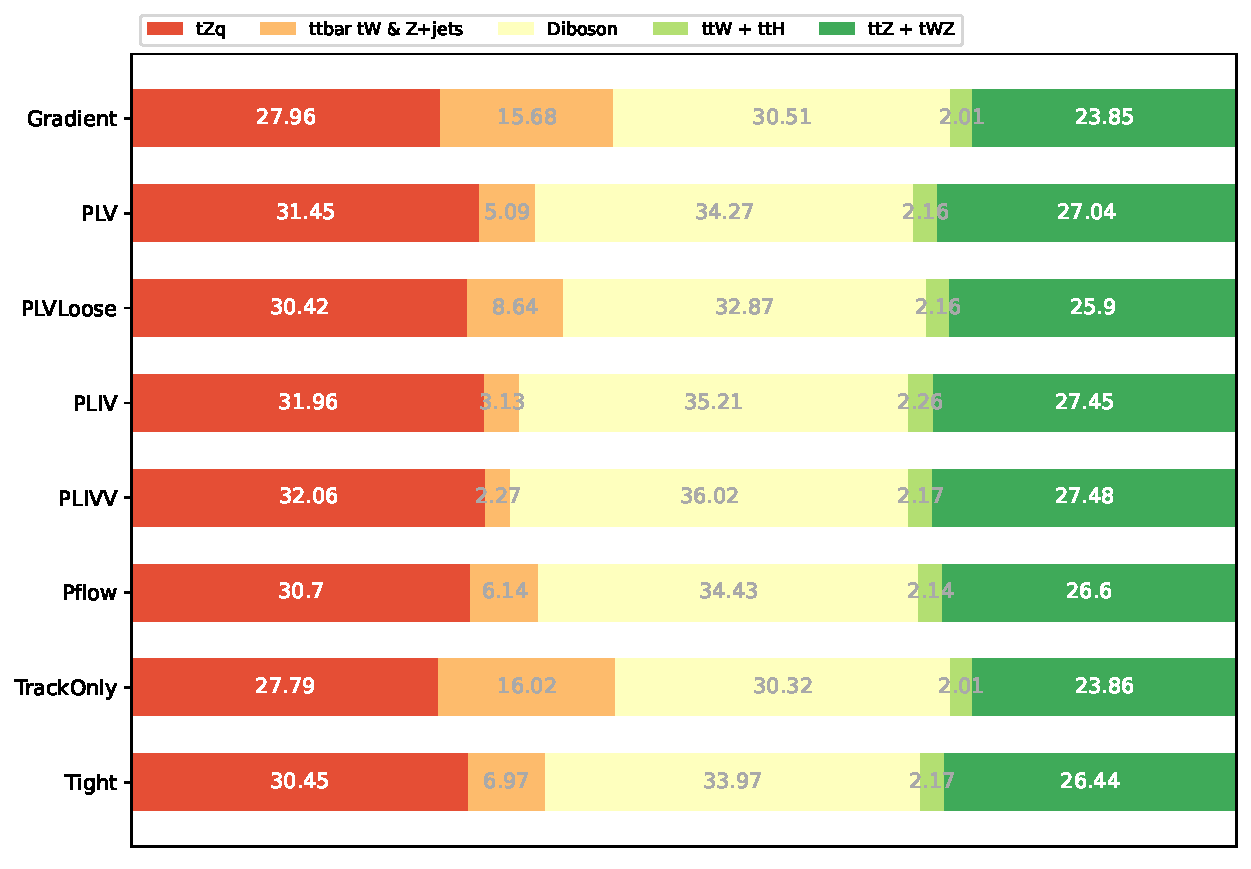
\includegraphics[width=0.85\textwidth]{ubonn-thesis/Chapters/Chapters_05/Figure/Lepton WPs/percent_plt_2j1b.pdf}
    \caption{Relative yield for SR 2j1b with jet $p_{T} > 35$ GeV, lepton $p_{T} >$ 28, 20, 20 , GeV \& btag-eff: 70\%}
    \label{fig:lep_wp_2j1b}
\end{figure}
 
\begin{figure}[h!]
    \centering
    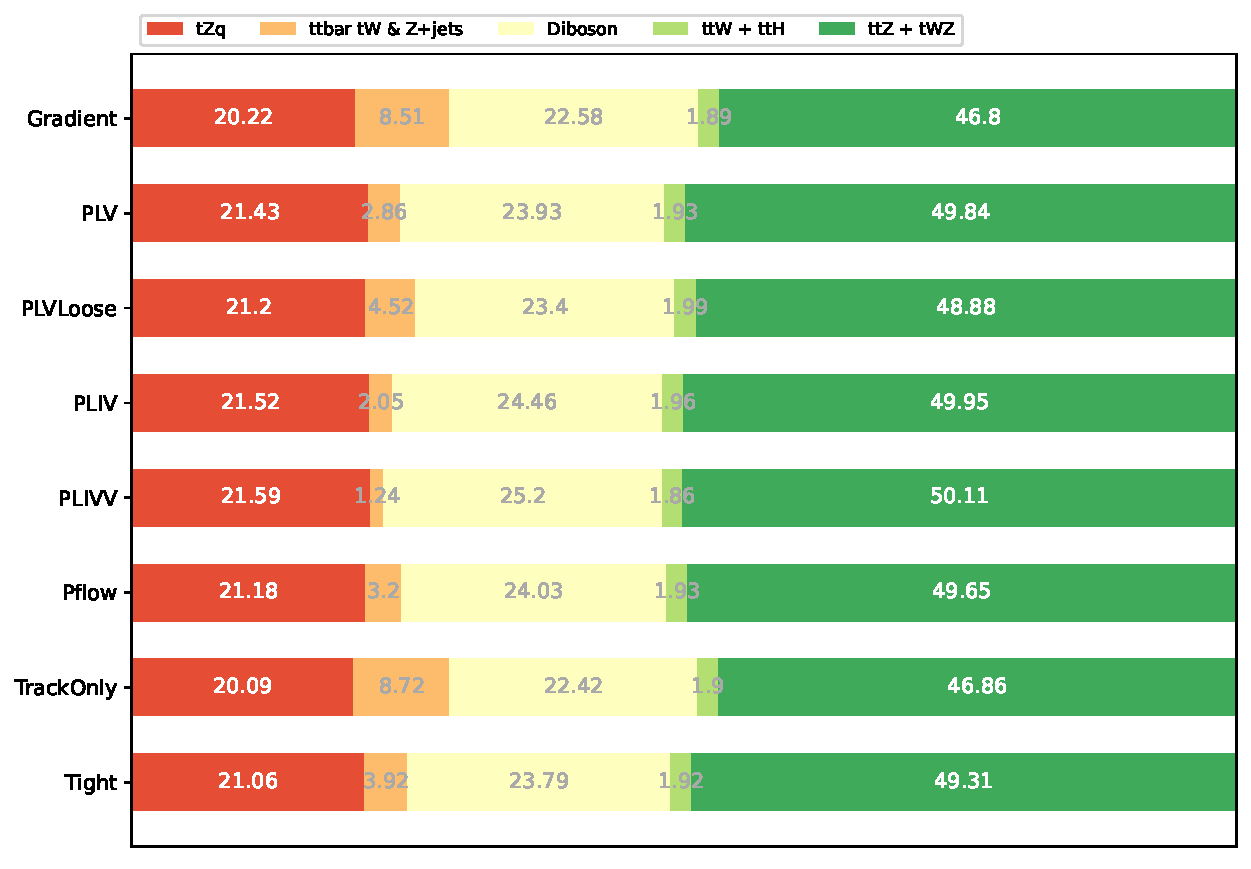
\includegraphics[width=0.85\textwidth]{ubonn-thesis/Chapters/Chapters_05/Figure/Lepton WPs/percent_plt_3j1b.pdf}
    \caption{Relative yield for SR 3j1b with jet $p_{T} > 35$ GeV, lepton $p_{T} >$ 28, 20, 20 , GeV \& btag-eff: 70\%}
    \label{fig:lep_wp_3j1b}
\end{figure}


In this analysis, the yield for a set of isolation WPs shown in the table \ref{tab:lep_wp} is presented. The yield are obtained with the following selection cuts: The three leptons are sorted by their $p_{T}$, irrespective of flavour, and required to have transverse momenta of at least 28, 20 and 20 GeV, respectively. Jets are required to have $P_{T} > 35$ GeV with one b-tagged jet with 70\% WP.


 Figures \ref{fig:lep_wp_2j1b} and \ref{fig:lep_wp_3j1b} show the relative yield for the different lepton WPs.  It is found that PLV, PLIV, and PLIVV have large signal and small fake-background compared to others. While PLVLoose has comparatively large fake background. The significance calculated in table \ref{tab:WP_sig} shows that PLVLoose has the highest significance for both SR-2j1b and SR-3j1b. The significance is also high for PLV and PLIV compared  to others. So, the lepton WPs: PLV, and PLVLoose are chosen for the optimization of selection cuts. 
 
\begin{table}[h!]
\centering
\begin{tabular}{@{} *8l  @{}}
\toprule
 & \multicolumn{3}{c}{SR 2j1b} & \multicolumn{3}{c}{SR 3j1b} \\
 \midrule
Lepton WPs & S & B & $\frac{S}{\sqrt{S+B}}$ & S & B & $\frac{S}{\sqrt{S+B}}$  \\ [0.2cm]
\toprule
 Gradient & 89.40 & 230.38 & 5.00 & 50.89 & 200.73 &  3.21  \\

PLV  & 83.73 & 182.51 &  5.13 & 47.67 & 174.82 &  3.20 \\ 

PLVLoose  & 91.50 & 209.26 &  5.28 & 52.10 & 193.61 &  3.32 \\

PLIV  & 80.70 & 171.8 &  5.08 & 46.10 & 168.10 &  3.15 \\ 

PLIVV  & 66.50 & 140.90 &  4.62 & 38.30 & 139.10 &  2.88 \\ 

Pflow & 79.86 & 180.27 & 4.95  & 45.79 & 170.38 & 3.11 \\

TrackOnly & 92.59 & 240.56 &  5.07 & 52.61 & 209.22 & 3.25 \\

Tight & 81.82 & 186.88 & 4.99 & 46.96 & 176.06 & 3.14  \\
\bottomrule
\end{tabular}
\caption{Values of the Significance for SR 2j1b and SR 3j1b for various isolation WPs}
\label{tab:WP_sig}
\end{table}  

%\newpage

%\newpage

\subsection{Optimization of cuts}
\label{subsec:Opti_cuts}

The analysis aims to set new requirements on the phase space so that the contribution of the signal grows relative to the number of background events. The significance is calculated for different selection cuts and are compared to the previous selections used in ref. \cite{tZq2020}. The cuts are optimized by varying leptons $p_{T}$, jets $p_{T}$ and the b-tagging efficiency of the b-tagged jet. The analysis framework uses the leptons sorted in $p_{T}$ ordered.

\vspace*{-0.2cm}
\begin{figure}[h!] 
  \begin{subfigure}[b]{0.49\linewidth}
    \centering
    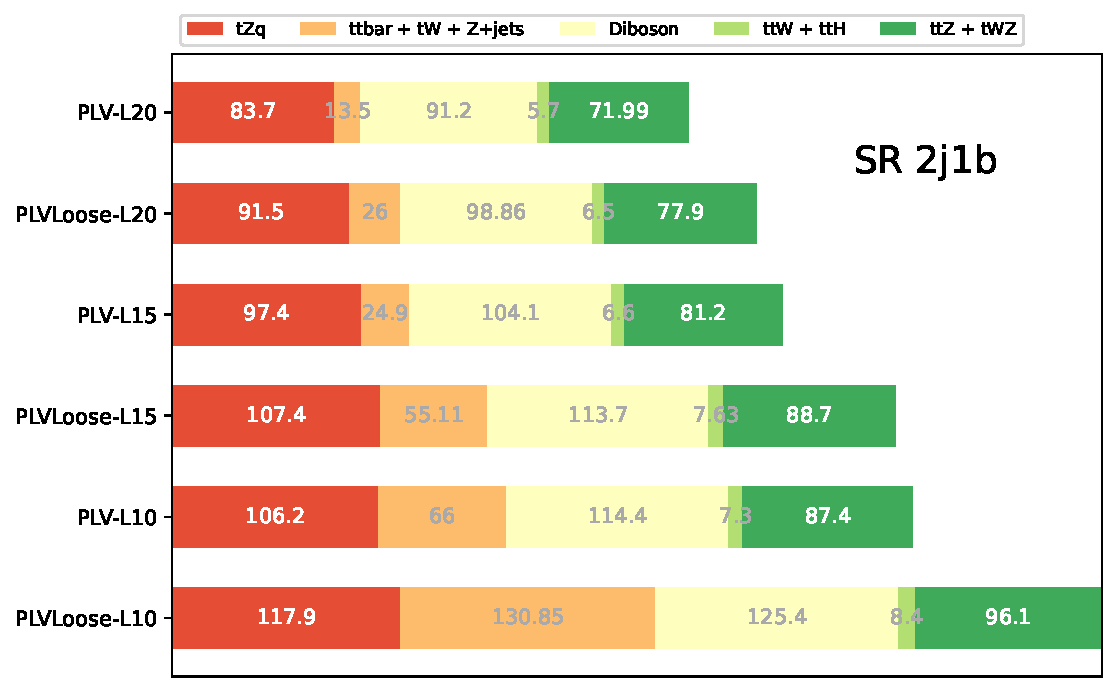
\includegraphics[width=\linewidth]{ubonn-thesis/Chapters/Chapters_05/Figure/Cuts Optimization/SR2j1b_PLVLoose.pdf}
    \end{subfigure}%% 
  \begin{subfigure}[b]{0.49\linewidth}
    \centering
    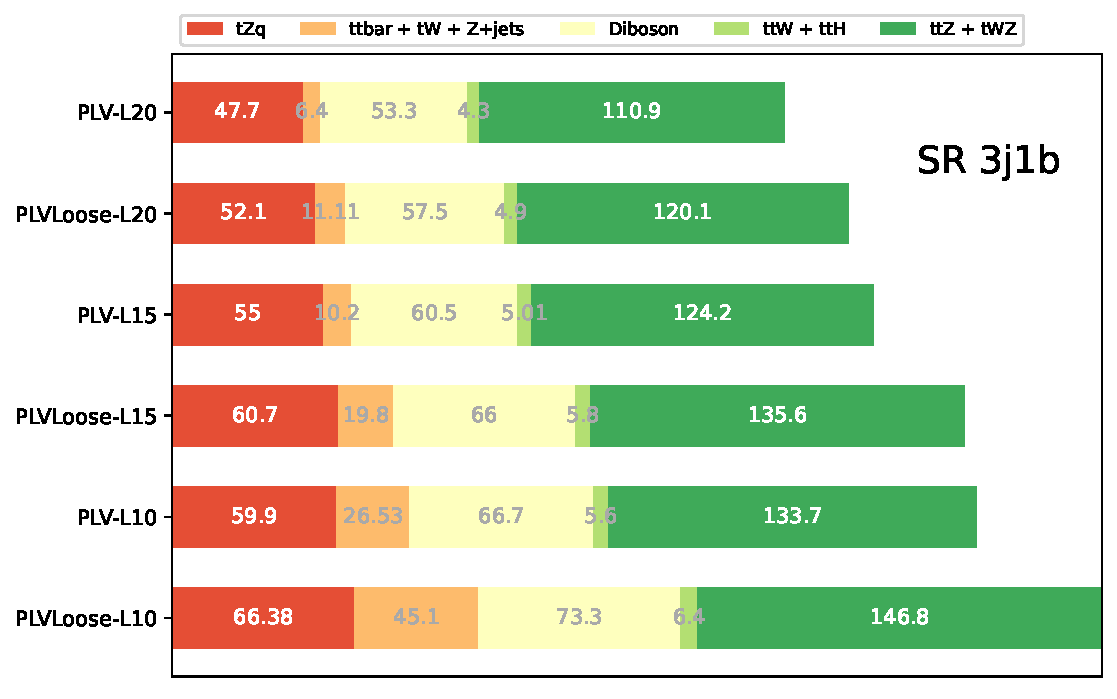
\includegraphics[width=\linewidth]{ubonn-thesis/Chapters/Chapters_05/Figure/Cuts Optimization/SR3j1b_PLVLoose.pdf} 
  \end{subfigure} 
  \vspace*{-0.2cm}
  \caption{Yield for signal and background at varying third lepton $p_{T}$ }
  \label{fig:third_lep}
  \end{figure}

\vspace*{-0.2cm}
\begin{table}[h!]
\centering
\begin{tabular}{@{} *8l  @{}}
\toprule
& & \multicolumn{3}{c}{SR 2j1b}  & \multicolumn{3}{c}{SR 3j1b}\\ 
 \midrule
Lepton WPs & $p_{T}(\ell_3) > $ & S & B & $\frac{S}{\sqrt{S+B}}$   & S & B & $\frac{S}{\sqrt{S+B}}$\\ [0.2cm]
\toprule
 \multirow{3}{*}{PLV} & $ \SI{20}{\GeV}$ & 83.70 & 182.39 &  5.13  & 47.7 & 174.9 &  3.20  \\

  & $ \SI{15}{\GeV}$ & 97.40 & 216.80 & 5.49 & 55.00 & 199.91 & 3.44  \\ 

 & $ \SI{10}{\GeV}$ & 106.40 & 275.10  & 5.45  & 59.90 & 232.53  & 3.50  \\
\midrule
 \multirow{3}{*}{PLVLoose} & $ \SI{20}{\GeV}$ & 91.50 & 209.26 & 5.28 & 52.10 & 193.61 & 3.32  \\

  & $ \SI{15}{\GeV}$ & 107.40 &  265.14 & 5.56 & 60.7 &  227.20 & 3.58  \\ 

 & $ \SI{10}{\GeV}$ & 117.90 & 360.75  & 5.35 & 66.38 & 271.60  & 3.61    \\
\bottomrule
\end{tabular}
\vspace*{-0.1cm}
\caption{Significance calculated at varying third lepton $p_{T}$ for both SR 2j1b and SR 3j1b}
\label{tab:third_lep_opt}
\end{table}

Figure \ref{fig:third_lep} shows the yield at varying third lepton $p_{T}$, while the first and third lepton lepton $p_{T}$ remain at 28 GeV and 20 GeV respectively. The btagging WP is 70\% and the jet transverse momentum remain above 30 GeV. It shows that both the signal and background increases with loose third lepton $p_{T}$ cut. The significance in table \ref{tab:third_lep_opt} that PLV at 10 GeV and PLVLoose at 15 GeV have considerable signal to background ratio while significance is above $5 \sigma$ for SR 2j1b and $3 \sigma$ for SR 3j1b. Figure \ref{fig:first_second_lepton_pt} shows that the change in the first lepton $p_{T}$ from 28 GeV to 27 GeV doesnot change the yield much for both PLV and PLVLoose. Similarly the yield remains same by changing the second lepton $p_{T}$ from 20 GeV to 15 GeV. Thus the final cut for analysis for the leptons $p_{T}$ are set to 27, 20, 10 GeV for PLV and 27, 20, 15 GeV for PLVLoose for first, second and third lepton $p_{T}$ respectively.

\begin{figure}[h!] 
  \begin{subfigure}[b]{0.49\linewidth}
    \centering
    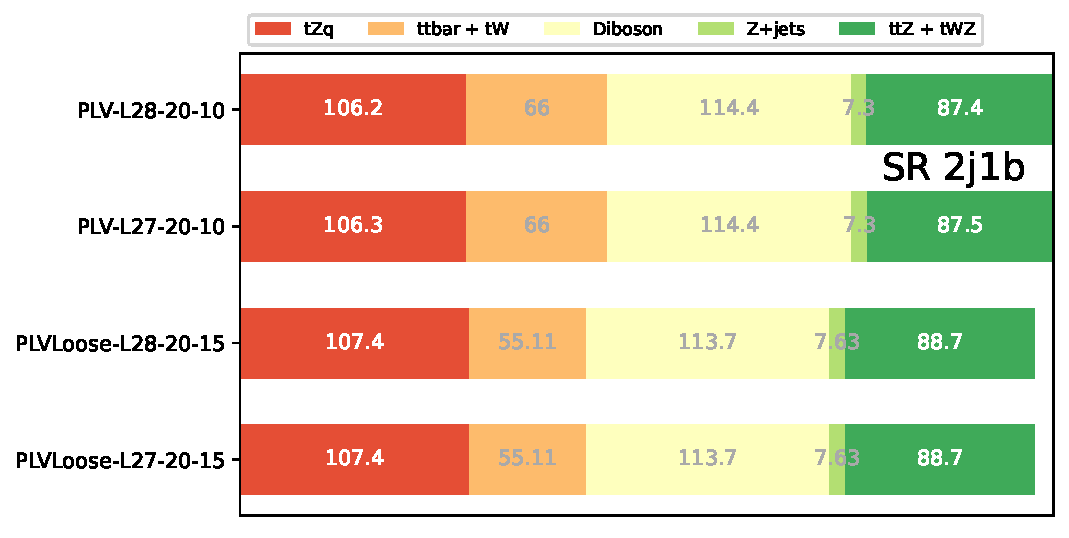
\includegraphics[width=\linewidth]{ubonn-thesis/Chapters/Chapters_05/Figure/Cuts Optimization/SR2j1b_PLVLoose_27.pdf} 
  \end{subfigure} 
  \hfill
  \begin{subfigure}[b]{0.49\linewidth}
    \centering
    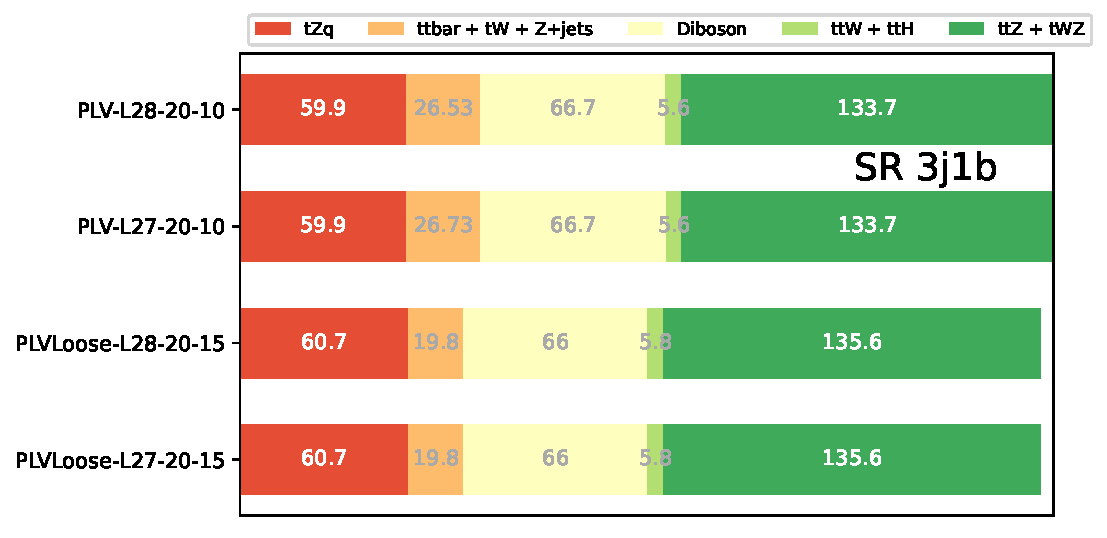
\includegraphics[width=\linewidth]{ubonn-thesis/Chapters/Chapters_05/Figure/Cuts Optimization/SR3j1b_PLVLoose_27.pdf} 
  \end{subfigure} 
  \caption{Events yield for signal and background at varying first lepton $p_{T}$ }
  \end{figure}
  \begin{figure}[h!] 
  \begin{subfigure}[b]{0.49\linewidth}
    \centering
    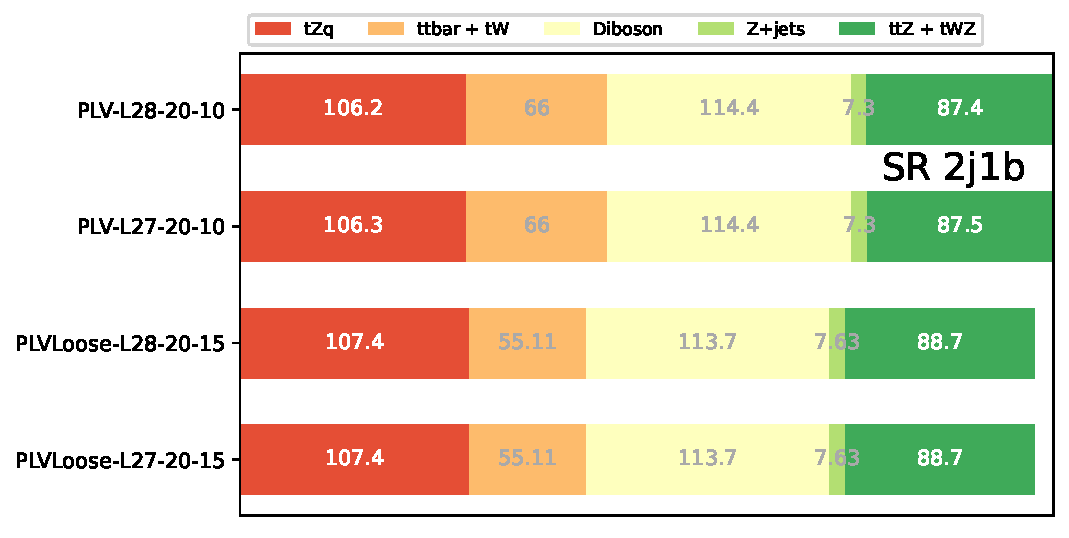
\includegraphics[width=\linewidth]{ubonn-thesis/Chapters/Chapters_05/Figure/Cuts Optimization/SR2j1b_PLVLoose_27.pdf} 
  \end{subfigure} 
  \hfill
  \begin{subfigure}[b]{0.49\linewidth}
    \centering
    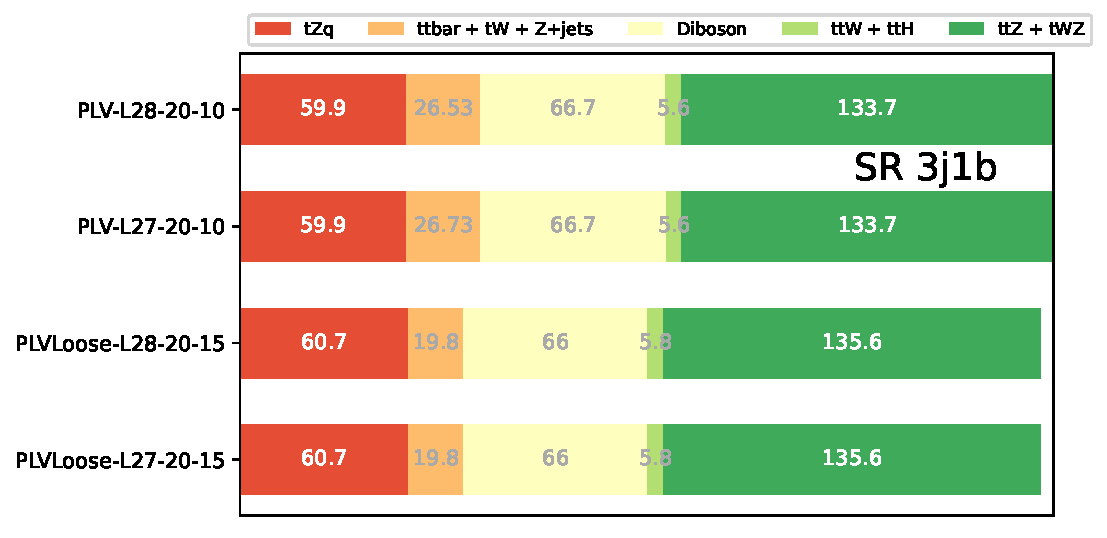
\includegraphics[width=\linewidth]{ubonn-thesis/Chapters/Chapters_05/Figure/Cuts Optimization/SR3j1b_PLVLoose_27.pdf} 
  \end{subfigure} 
  \caption{Events yield for signal and background at varying second lepton $p_{T}$}
  \label{fig:first_second_lepton_pt}
  \end{figure}
 
Figures \ref{fig:SR_2j1bbtag} and \ref{fig:SR_3j1btag} show the yield at varying jet $p_{T}$, b-tagging efficiency and third lepton $p_{T}$. The lower in jet $p_{T}$ migrate the signal to higher jet multiplicity keeping total number of signal in SR 2j1b and SR 3j1b nearly same. There is large increase in diboson background yield with increase in b-tagging working point. Here, in the plot the diboson contribution is split according to the origin of the associated jets using generator-level information. If one of the jets contains a b- or c-hadron then it is classified as diboson + heavy flavour (VV + HF), otherwise the event is classified as diboson + light flavour (VV + LF). Thus for final cut for the jet transverse momentum and b-jet tagging efficiency for our analysis remain at 35 GeV and 70\%. 

\begin{figure}[h!]
    \centering
    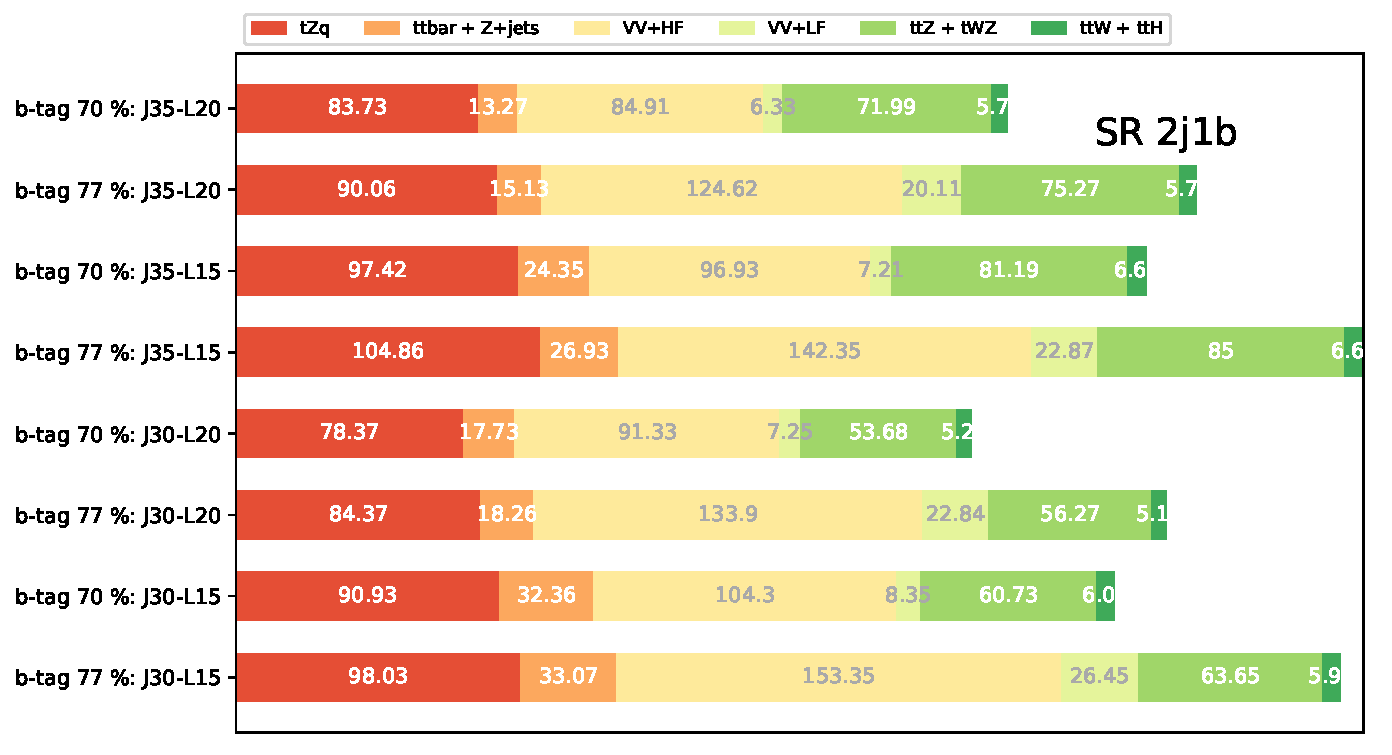
\includegraphics[width=0.75\textwidth]{ubonn-thesis/Chapters/Chapters_05/Figure/Cuts Optimization/jet_2j1b_yield.pdf}
    \caption{Events yeild for signal and background obtained by varing the jet $p_{T}$, b-tagging efficiency and the third lepton $p_{T}$ in the SR 2j1b}
    \label{fig:SR_2j1bbtag}
\end{figure}

\begin{figure}[h!]
    \centering
    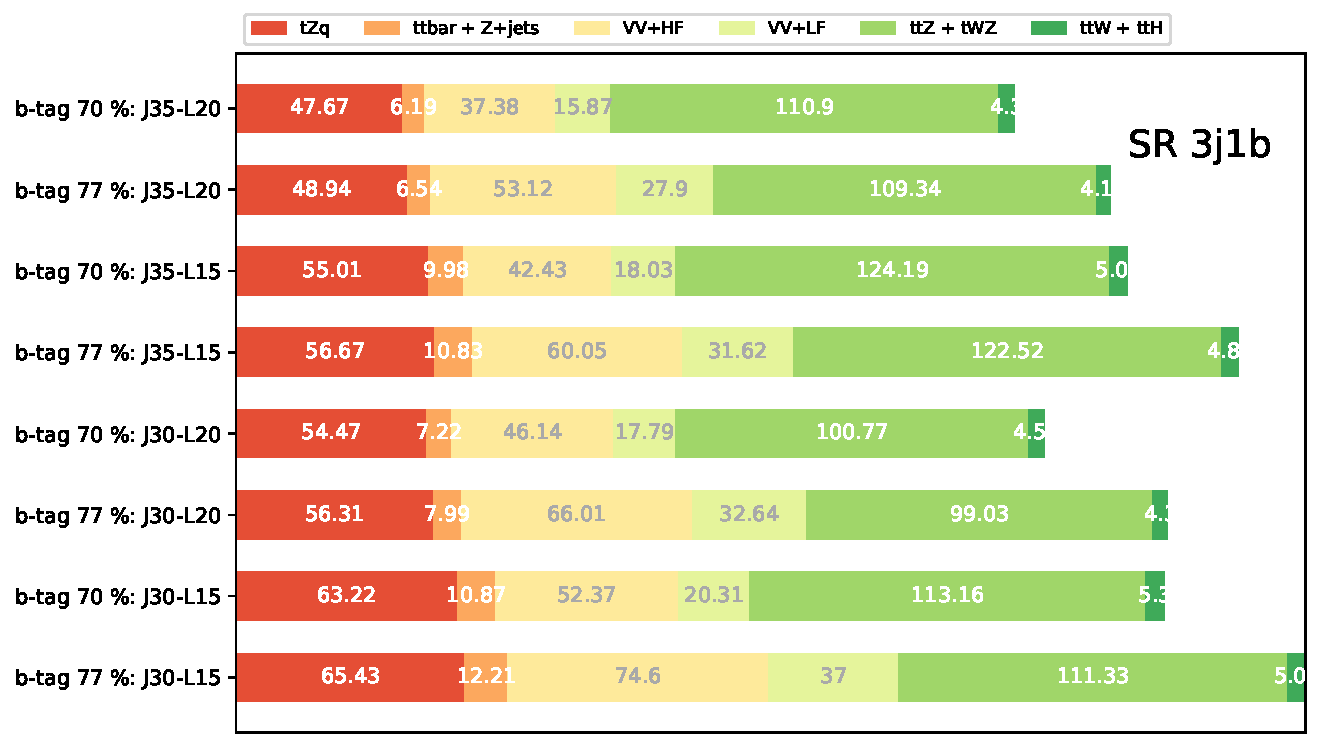
\includegraphics[width=0.75\textwidth]{ubonn-thesis/Chapters/Chapters_05/Figure/Cuts Optimization/jet_3j1b_yield.pdf}
    \caption{Events yeild for signal and background obtained by varing the jet $p_{T}$, b-tagging efficiency and the third lepton $p_{T}$ in the SR 3j1b}
    \label{fig:SR_3j1btag}
\end{figure}



\subsection{Signal regions (SRs) plots and yields}
\label{subsec:SR_plot_yield}

The regions are constructed as described in section \ref{sec:SR}. The full selection cuts applied in the signal regions are listed in table \ref{tab:final_selection}. In this table, the selection cuts for the definition of control regions are  

\begin{table}[hbt!]
\centering
\begin{tabular}{@{} *4l  @{}}
\toprule
& \multicolumn{2}{c}{Common selections} & \\
\midrule
& \multicolumn{2}{c}{Exactly 3 leptons ($e$ or $\mu$) with $|\eta| < 2.5$} &  \\
& \multicolumn{2}{c}{$p_{T}(\ell_1)> \SI{27}{\GeV}$, $p_{T}(\ell_2)> \SI{20}{\GeV}$, $p_{T}(\ell_3)> \SI{10}{\GeV}$} &  \\
& \multicolumn{2}{c}{$p_{T}(\text{jet})> \SI{35}{\GeV}$} &  \\[0.3em]
\toprule
SR 2j1b  & CR Diboson 2j0b & CR $t\Bar{t}Z$ 3j2b & CR $t\Bar{t}$ 2j1b  \\
\midrule
$\ge$ 1 OSSF pair & $\ge$ 1 OSSF pair & $\ge$ 1 OSSF pair & $\ge$ 1 OSDF pair  \\
$|m_{\ell \ell} - m_{Z}| <  \SI{10}{\GeV}$ & $|m_{\ell \ell} - m_{Z}| < $ \SI{10}{\GeV} & $|m_{\ell \ell} - m_{Z}| < $ \SI{10}{\GeV} & No OSSF pair  \\
2 jets, $|\eta| < $ 4.5  & 2 jets, $|\eta| < $ 4.5  & 3 jets, $|\eta| < $ 4.5 & 2 jets, $|\eta| < $ 4.5  \\
1 bjet, $|\eta| < $ 2.5 & 0 bjets & 2 bjets, $|\eta| < $ 2.5  & 1 bjet, $|\eta| < $ 2.5   \\[0.3em]
\toprule
SR 3j1b   & CR Diboson 3j0b & CR $t\Bar{t}Z$ 4j2b & CR $t\Bar{t}$ 3j1b \\
\midrule
$\ge$ 1 OSSF pair & $\ge$ 1 OSSF pair & $\ge$ 1 OSSF pair & $\ge$ 1 OSDF pair \\
$|m_{\ell \ell} - m_{Z}| <  \SI{10}{\GeV}$ & $|m_{\ell \ell} - m_{Z}| < $ \SI{10}{\GeV} & $|m_{\ell \ell} - m_{Z}| < $ \SI{10}{\GeV} & No OSSF pair  \\
3 jets, $|\eta| < $ 4.5  & 3 jets, $|\eta| < $ 4.5  & 4 jets, $|\eta| < $ 4.5 & 3 jets, $|\eta| < $ 4.5  \\
1 bjet, $|\eta| < $ 2.5 & 0 bjets  & 2 bjets, $|\eta| < $ 2.5  & 1 bjet, $|\eta| < $ 2.5   \\
\bottomrule
\end{tabular}
\caption{Overview of the requirements applied when selecting events in the signal and control regions. OSSF is an opposite-sign same-flavour lepton pair. OSDF is an opposite-sign different-flavour lepton pair.}
\label{tab:final_selection}
\end{table}
 
also reported. The event yields in the SRs after the full selection can be found in table \ref{tab:yield_SR} and histogram distributions of reconstructed variables from the top quark and Z boson are given in figure \ref{fig:signal}. The predicted number of events to pass selection cuts based on MC simulations for tZq as well as all previously mentioned backgrounds are tabulated. The events in these regions are the primary regions of interest for the statistical analysis described in section \ref{sec: Profile_likehihood} after having been evaluated by the neural network described in section \ref{sec:NN}.

\begin{table}[!h]
    \begin{minipage}{.49\textwidth}
      \centering
      \begin{adjustbox}{width=\textwidth}
       \begin{tabular}{@{} *3l @{}}
 \toprule
 Process & Number of events & Number of raw events  \\ [0.5ex] 
 \hline\hline
  tZq   & 97.46 \pm 0.67 & 56838800 \\ 
  tt   & 22.72 \pm 0.88  & 104389 \\ 
  tW   & 0.89 \pm 0.61   & 1112 \\ 
  Z+jets   & 36.66 \pm 4.13 & 228516 \\ 
  Diboson   & 115.60 \pm 1.09  & 5741400 \\ 
  ttZ   & 62.88 \pm 2.30 & 7001290  \\ 
  ttW   & 4.56 \pm 0.18 & 255621  \\ 
  tWZ   & 19.34 \pm 0.58 & 489419 \\ 
  ttH   & 2.11 \pm 0.04   & 715711 \\ 
\hline 
  Total expected  & 362.22 \pm 4.65 & 71376200 \\ 
\hline 
  Data   & 443  & 443  \\   
 \bottomrule
 \end{tabular} 
 \end{adjustbox}
    \end{minipage}%
    \hfill
    %\hspace{-1.5cm}
    \begin{minipage}{.49\textwidth}
      \centering
      \vspace*{0.5cm}
      \begin{adjustbox}{width=\textwidth}
        \begin{tabular}{@{} *3l @{}}
 \toprule
 Process & Number of events & Number of raw events  \\ [0.5ex] 
 \hline\hline
   tZq   &  55.31 \pm 0.56 & 38569200 \\ 
  tt   & 10.79 \pm 0.61 & 49206 \\ 
  tW   & 0.33 \pm 0.58 & 417 \\ 
  Z+jets & 13.32 \pm 1.14 & 102582 \\ 
  Diboson  & 66.05 \pm 0.70 & 3615390 \\ 
  ttZ   & 101.39 \pm 0.68 & 12441100 \\ 
  ttW   & 2.34 \pm 0.13 & 134969 \\ 
  tWZ   & 22.92 \pm 0.65 & 596449 \\ 
  ttH   & 2.80 \pm 0.05  & 753658 \\ 
\hline 
  Total expected  & 275.24 \pm 1.84 & 56262900 \\ 
\hline 
  Data    & 307 & 307 \\ 
 \bottomrule
 \end{tabular} 
 \end{adjustbox}
\end{minipage} 
\caption{Numbers of expected events in the SR 2j1b (Left) and SR 3j1b (Right) broken down by process. The uncertainty shown contains only the statistical component.}
\label{tab:yield_SR}
\end{table}


\begin{figure}[h!] 
  \begin{subfigure}[b]{0.33\linewidth}
    \centering
    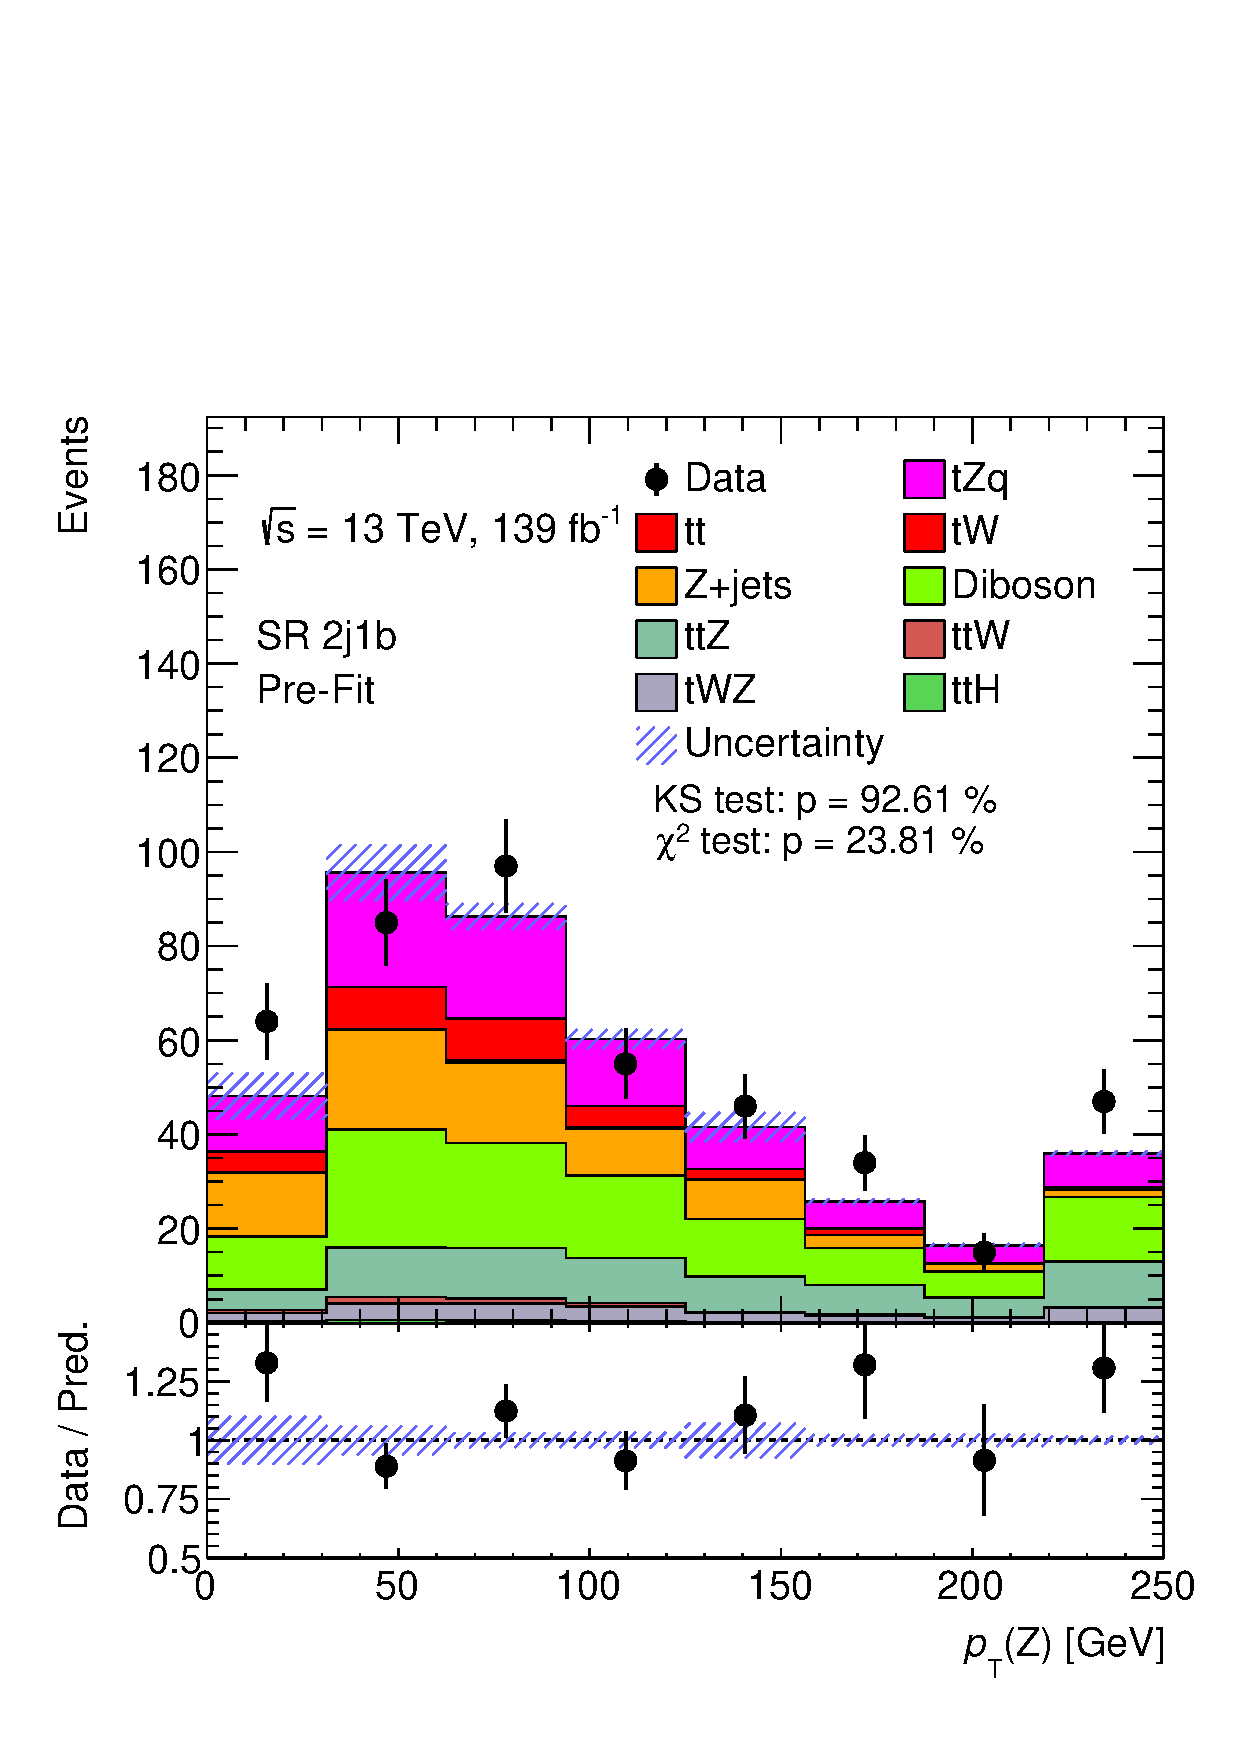
\includegraphics[width=\linewidth]{ubonn-thesis/Chapters/Chapters_05/Figure/SR/SR_2j1b_Z_pt.pdf} 
  \end{subfigure}%% 
  \begin{subfigure}[b]{0.33\linewidth}
    \centering
    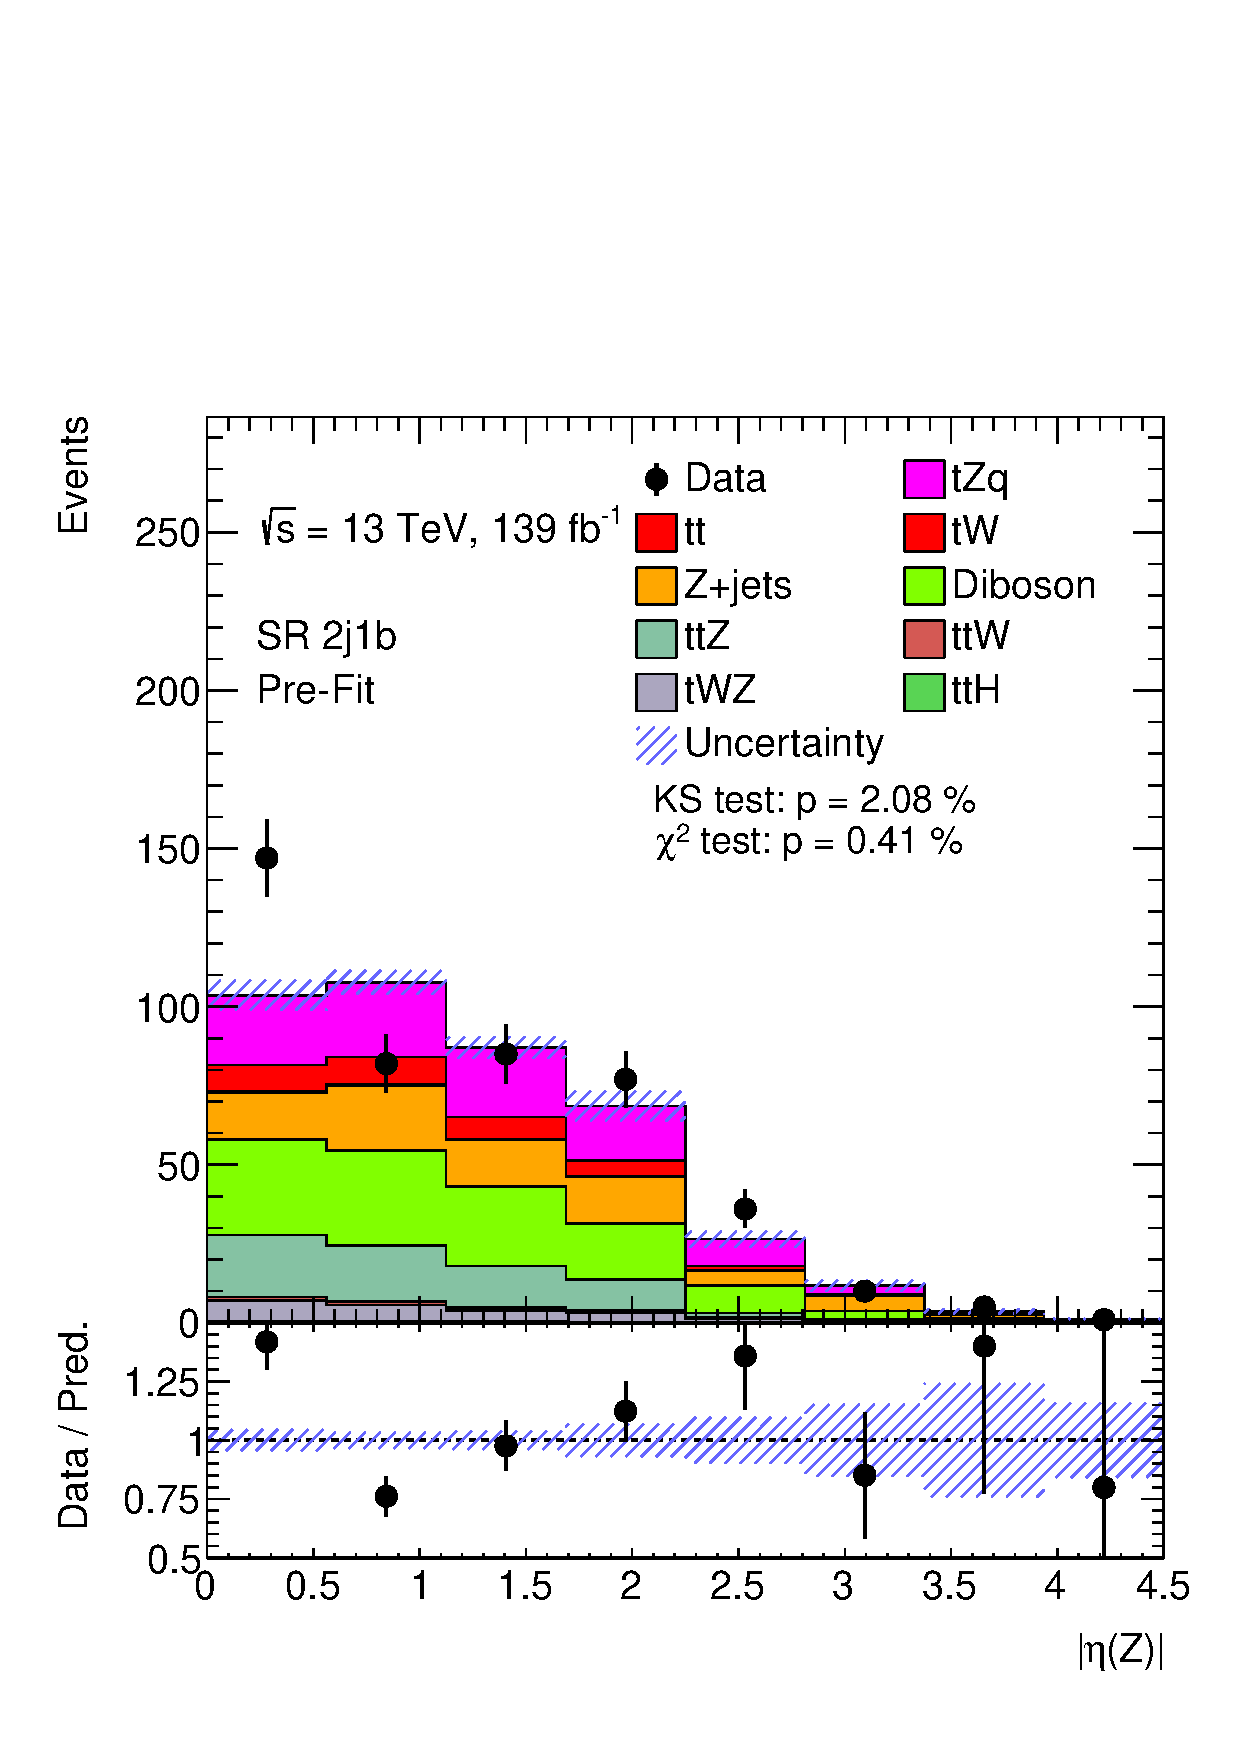
\includegraphics[width=\linewidth]{ubonn-thesis/Chapters/Chapters_05/Figure/SR/SR_2j1b_Z_eta.pdf} 
  \end{subfigure} 
  \begin{subfigure}[b]{0.33\linewidth}
    \centering
    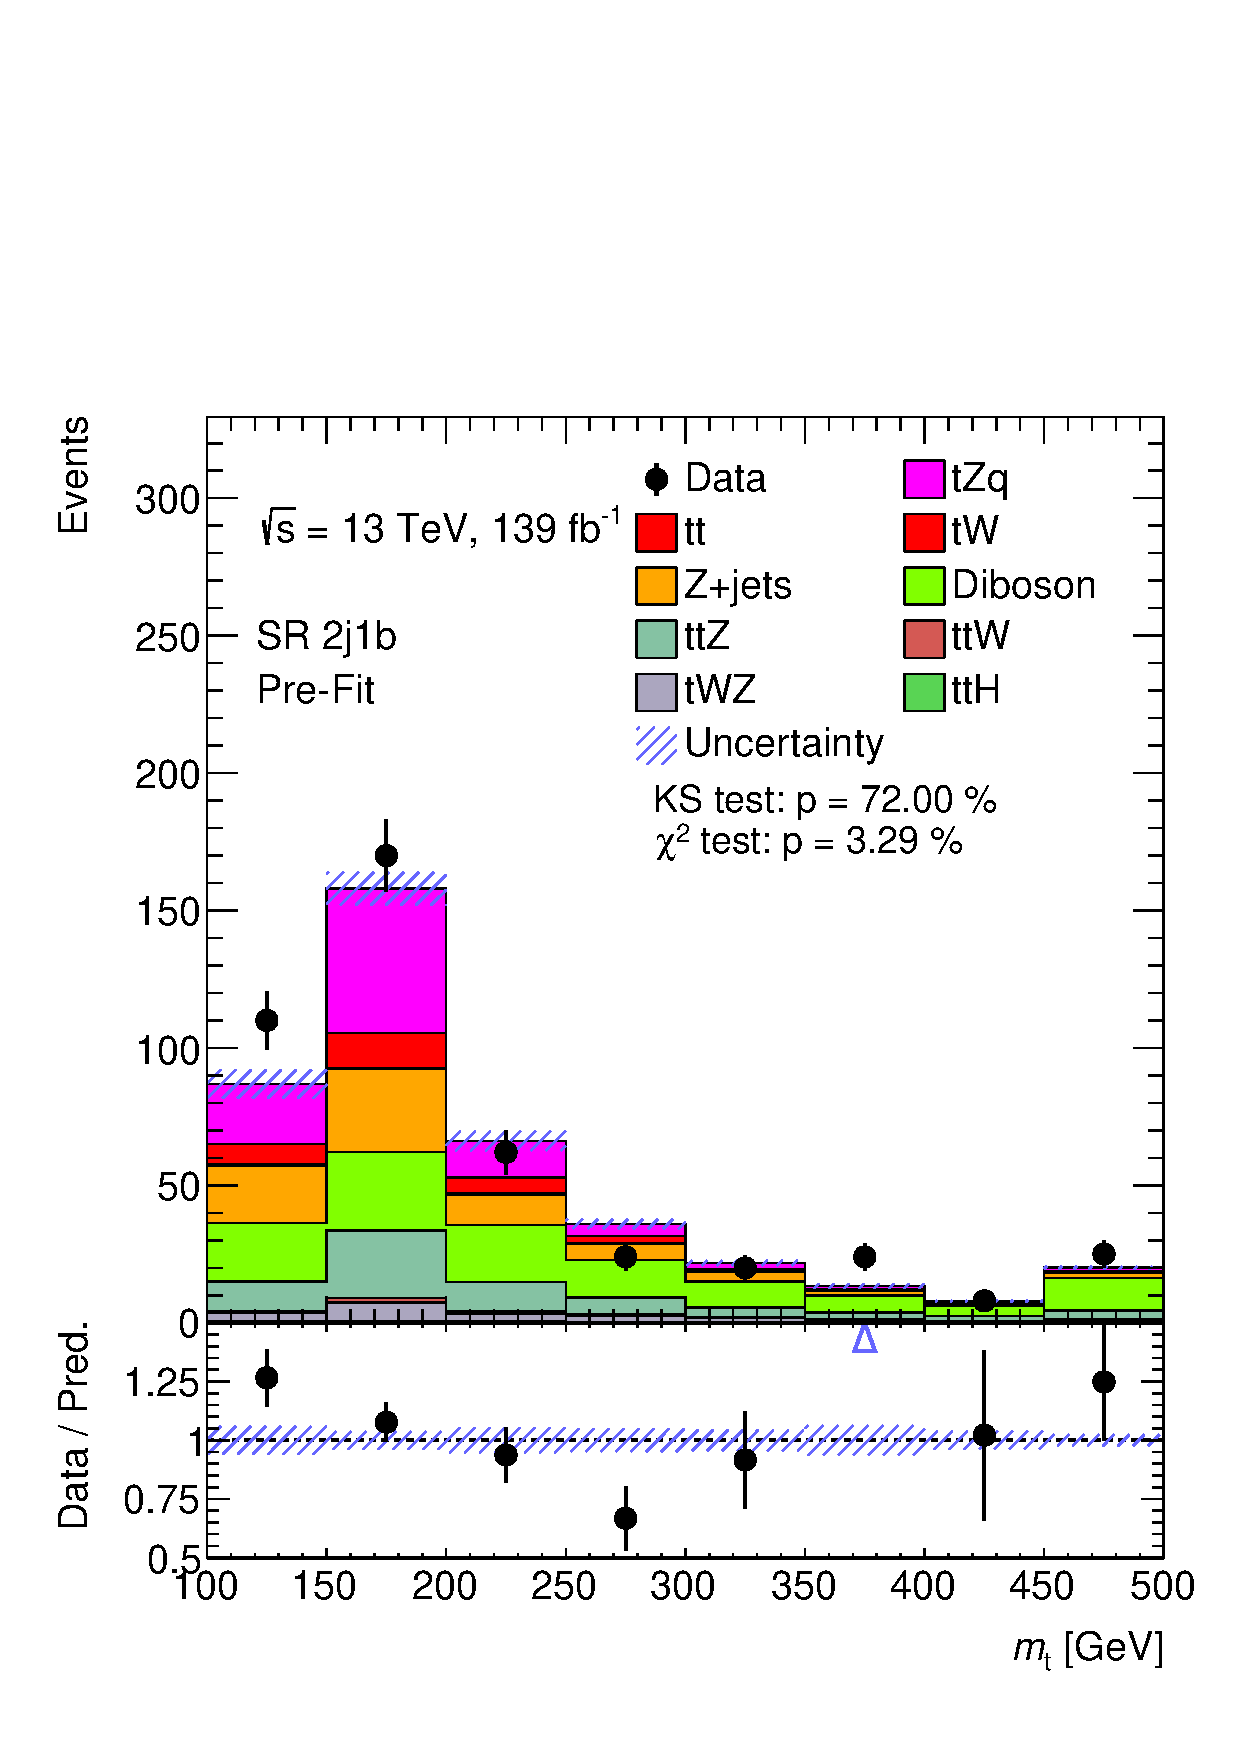
\includegraphics[width=\linewidth]{ubonn-thesis/Chapters/Chapters_05/Figure/SR/SR_2j1b_Top_mass.pdf} 
  \end{subfigure}%%
  \newline
  \begin{subfigure}[b]{0.33\linewidth}
    \centering
    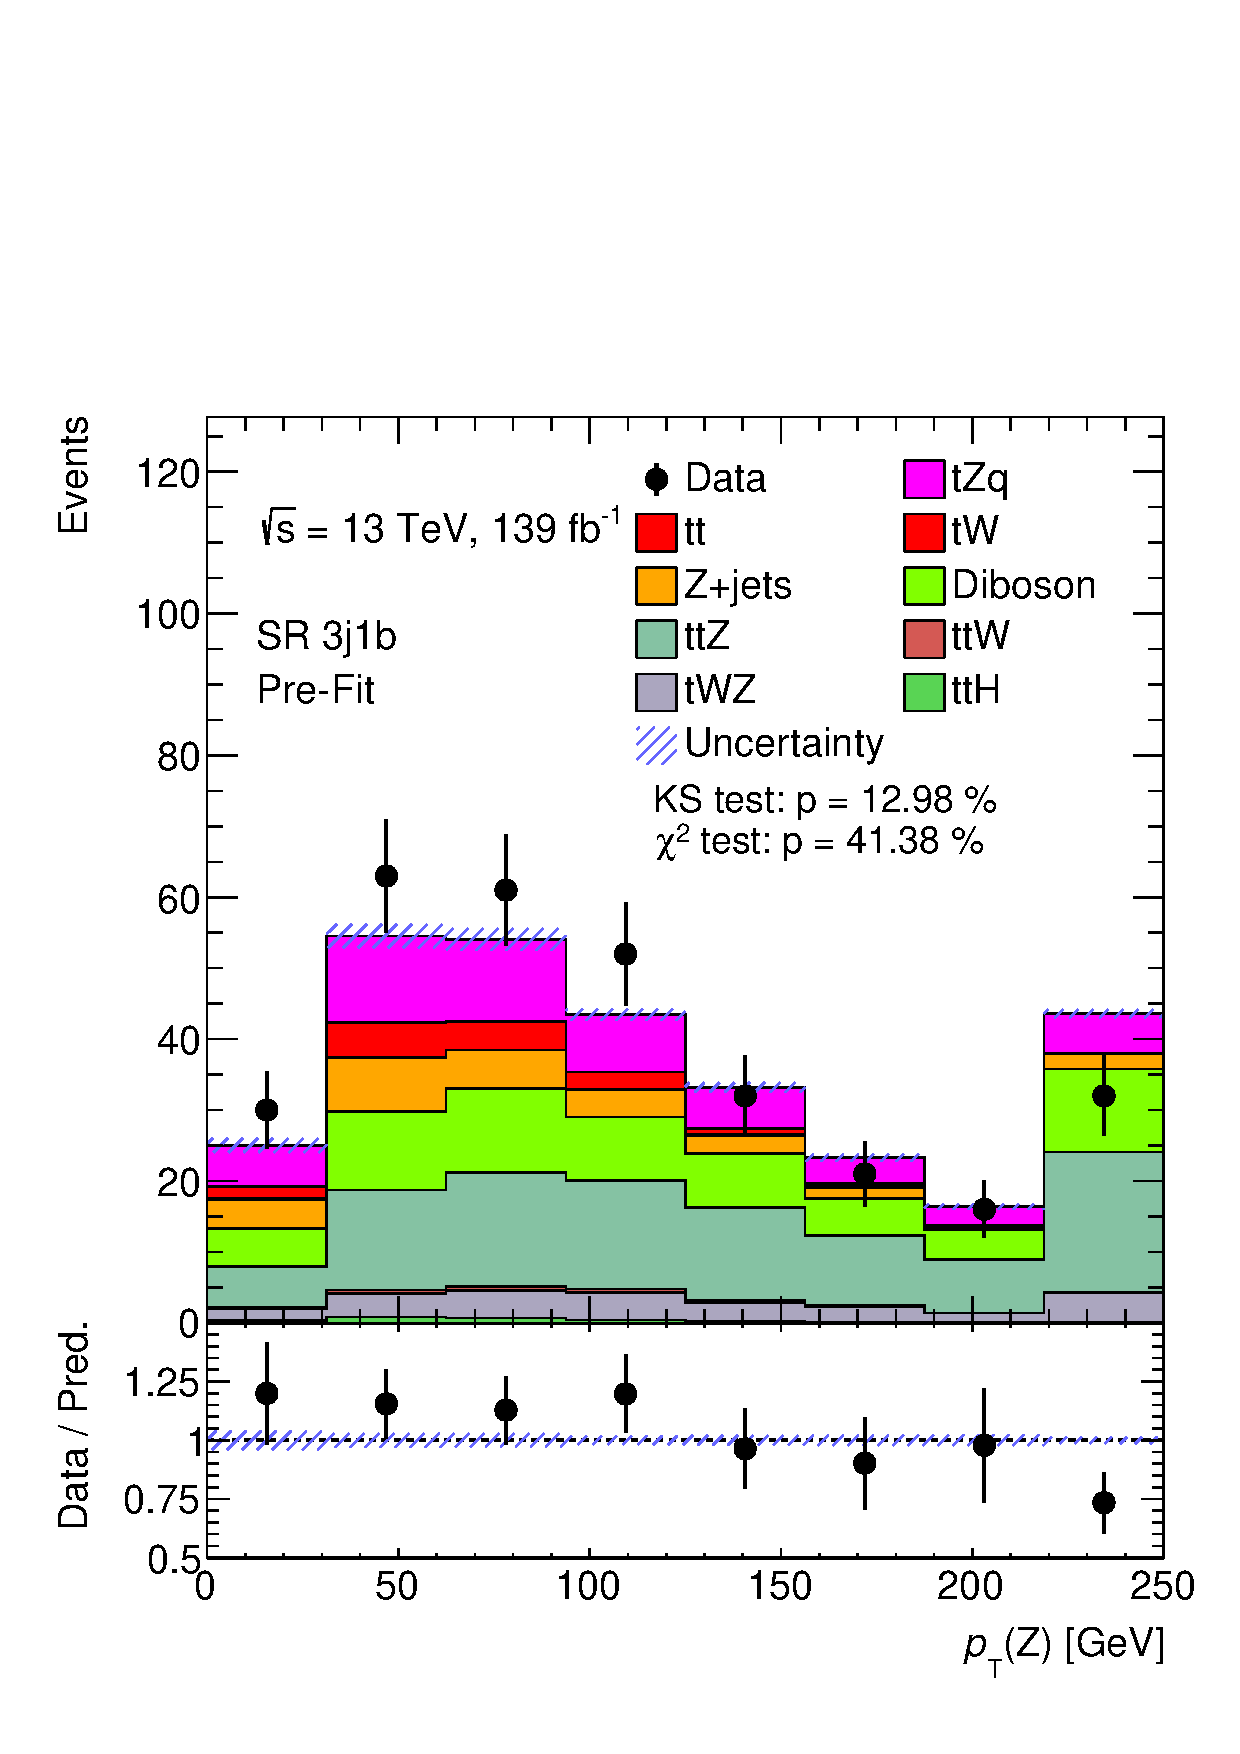
\includegraphics[width=\linewidth]{ubonn-thesis/Chapters/Chapters_05/Figure/SR/SR_3j1b_Z_pt.pdf} 
  \end{subfigure}%%
  \begin{subfigure}[b]{0.33\linewidth}
    \centering
    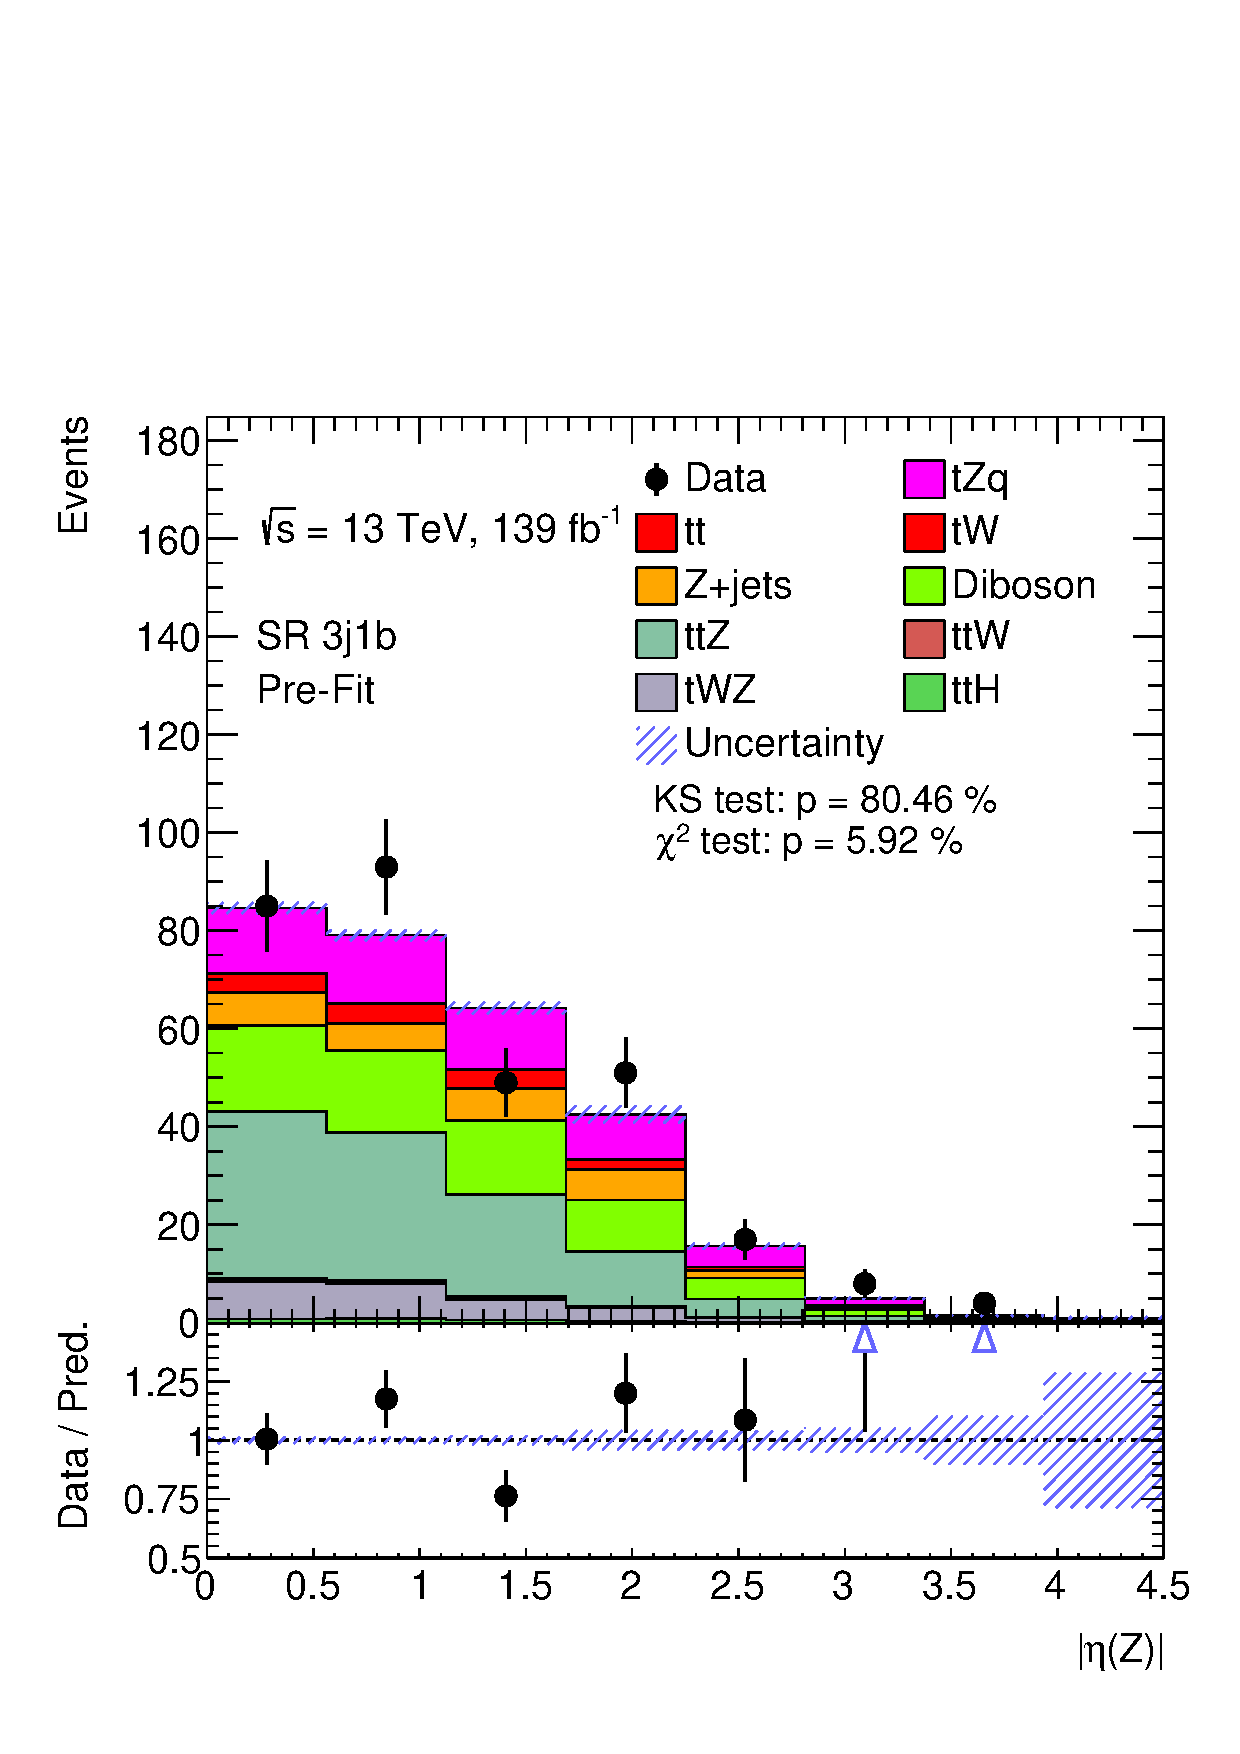
\includegraphics[width=\linewidth]{ubonn-thesis/Chapters/Chapters_05/Figure/SR/SR_3j1b_Z_eta.pdf} 
  \end{subfigure}
  \begin{subfigure}[b]{0.33\linewidth}
    \centering
    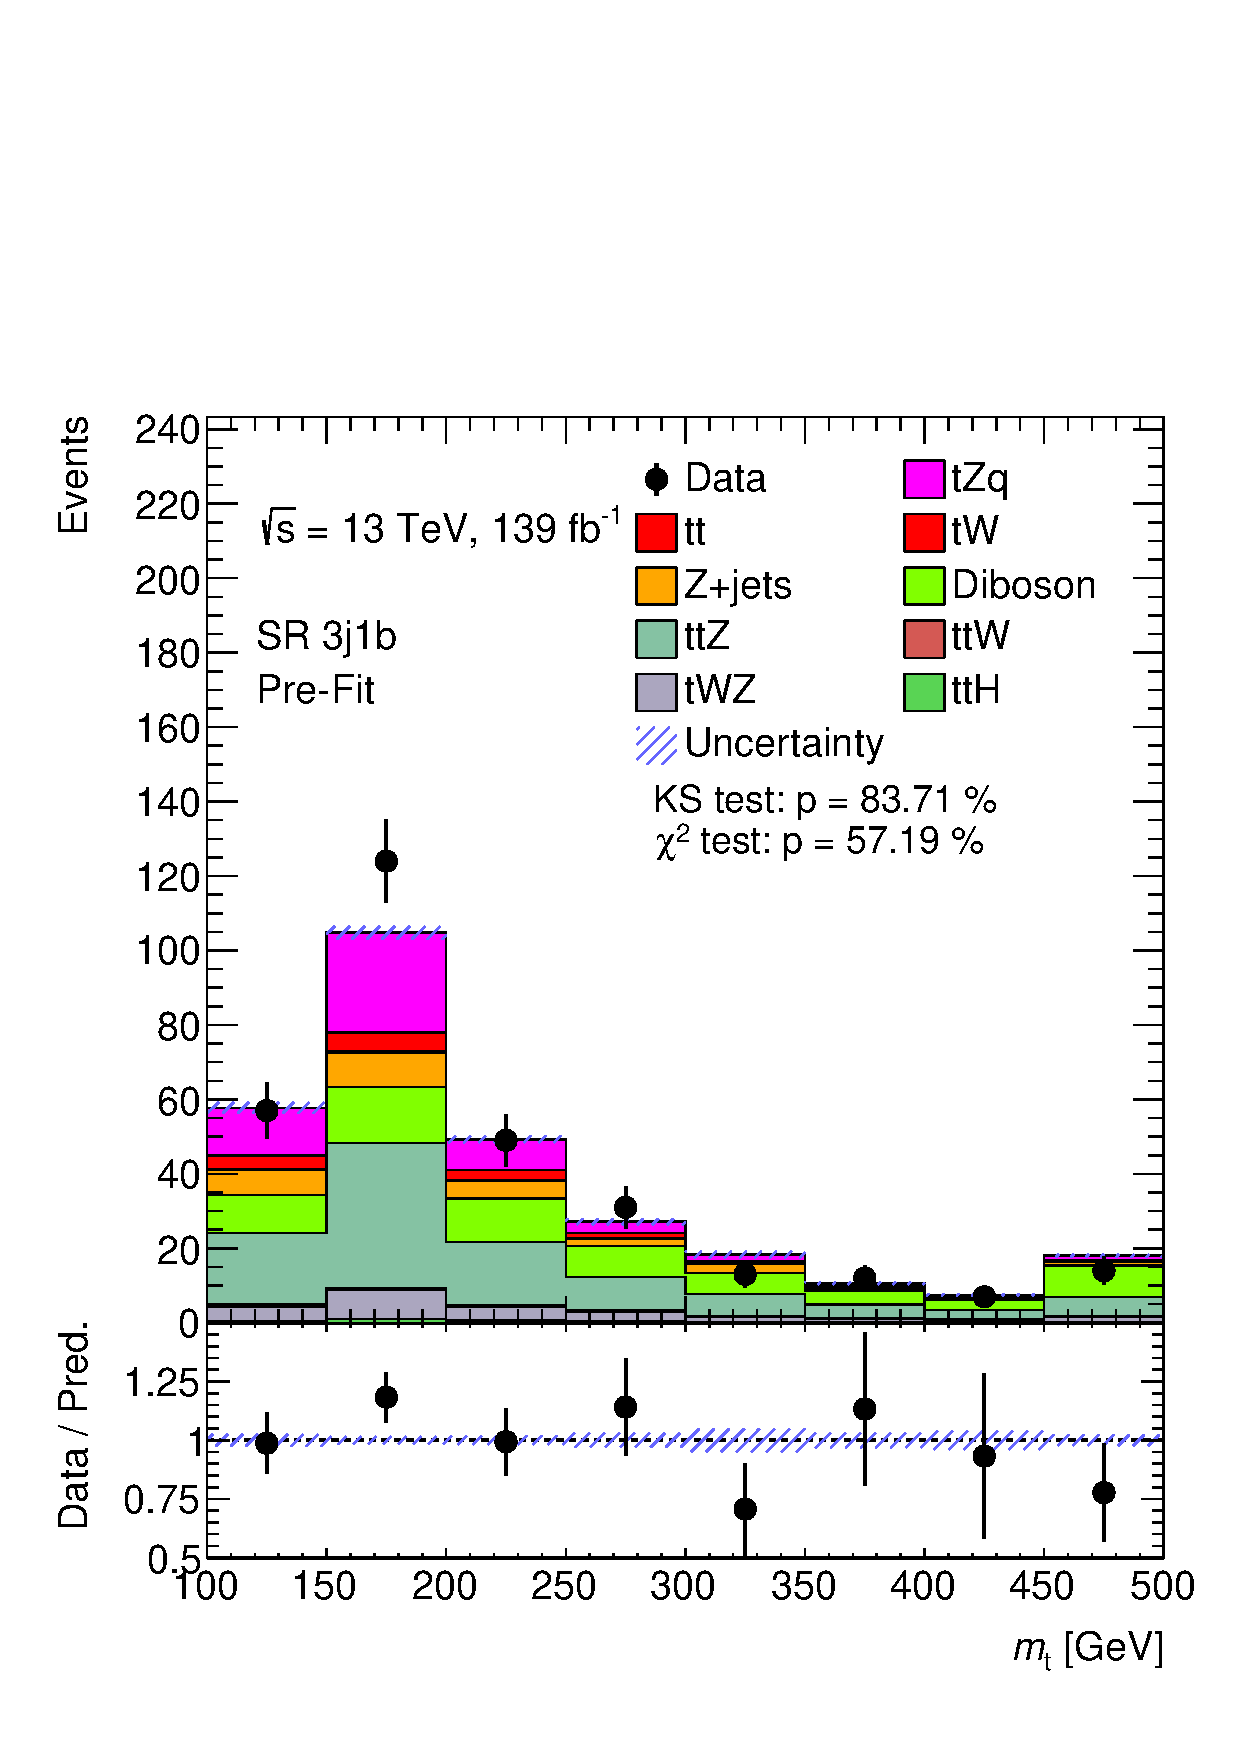
\includegraphics[width=\linewidth]{ubonn-thesis/Chapters/Chapters_05/Figure/SR/SR_3j1b_Top_mass.pdf} 
  \end{subfigure} 
  \caption{Comparison of data and MC predictions for reconstructed event related quantities for events in the SR 2j1b and SR 3j1b. The uncertainty shown is the statistical uncertainty}
  \label{fig:signal} 
\end{figure}






\section{Control regions (CRs)}
\label{sec:CR}

In order to ensure proper modeling of each relevant background, a series of control regions as listed in table \ref{tab:final_selection} are defined. These regions are constructed such that they are enriched in three of the main sources of backgrounds: diboson, $t\Bar{t}Z$, and $t\Bar{t}$ production. There are two CRs for each background, and one corresponding to each signal region.

\subsection{Diboson CRs plots and yields}
\label{subsec:diboson_plot_yield}

To define regions of phase space enriched in diboson production, the b-jet is vetoed. This leads to events such as WZ to dominate while effectively removing the events containing the top quark. This region also has significant contamination from Z+jets events. 

\begin{table}[!h]
    \begin{minipage}{.49\textwidth}
      \centering
      \begin{adjustbox}{width=\textwidth}
       \begin{tabular}{@{} *3l @{}}
 \toprule
 Process & Number of events & Number of raw events  \\ [0.5ex] 
 \hline\hline
  tZq   &  61.94 \pm 0.57 & 40215200 \\ 
  tt   &  14.58 \pm 0.73 & 64357  \\ 
  tW   & 0.49 \pm 0.75   &  556 \\ 
  Z+jets   & 152.32 \pm 18.75 & 624666  \\ 
  Diboson   & 2625.59 \pm 5.02  & 146163000  \\ 
  ttZ   & 48.59 \pm 4.79 &  4766730 \\ 
  ttW   & 1.85 \pm 0.11 & 98134 \\ 
  tWZ   & 17.10 \pm 0.54 & 422977 \\ 
  ttH   & 1.14 \pm 0.03   & 323175 \\ 
\hline 
  Total expected  & 2923.59 \pm 17.11  & 192679000 \\ 
\hline 
  Data   & 3116   & 3116 \\  
 \bottomrule
 \end{tabular} 
 \end{adjustbox}
    \end{minipage}%
    \hfill
    %\hspace{-1.5cm}
    \begin{minipage}{.49\textwidth}
      \centering
      \vspace*{0.5cm}
      \begin{adjustbox}{width=\textwidth}
        \begin{tabular}{@{} *3l @{}}
 \toprule
 Process & Number of events & Number of raw events  \\ [0.5ex] 
 \hline\hline
   tZq   &  25.58 \pm 0.42 & 21530100 \\ 
  tt   & 5.59 \pm 0.46 & 24603  \\ 
  tW   & 0.60 \pm 0.42 & 695 \\ 
  Z+jets & 52.53 \pm 5.89  & 244640  \\ 
  Diboson  & 973.45 \pm 2.35 & 60037700 \\ 
  ttZ   & 47.15 \pm 1.42 & 6095710 \\ 
  ttW   & 0.88 \pm 0.09 & 51847  \\ 
  tWZ   & 13.13 \pm 0.51  & 375439 \\ 
  ttH   & 1.07 \pm 0.03 & 268270 \\ 
\hline 
  Total expected  & 1119.97 \pm 6.51 & 88629000 \\ 
\hline 
  Data    & 1083 & 1083 \\ 
 \bottomrule
 \end{tabular} 
 \end{adjustbox}
    \end{minipage} 
    \caption{Numbers of expected events in the CR 2j0b (Left) and CR 3j0b (Right) broken down by process. The uncertainty shown contains only the statistical component.}
 \label{tab:yield_diboson}
\end{table}


\begin{figure}[h!] 
  \begin{subfigure}[b]{0.33\linewidth}
    \centering
    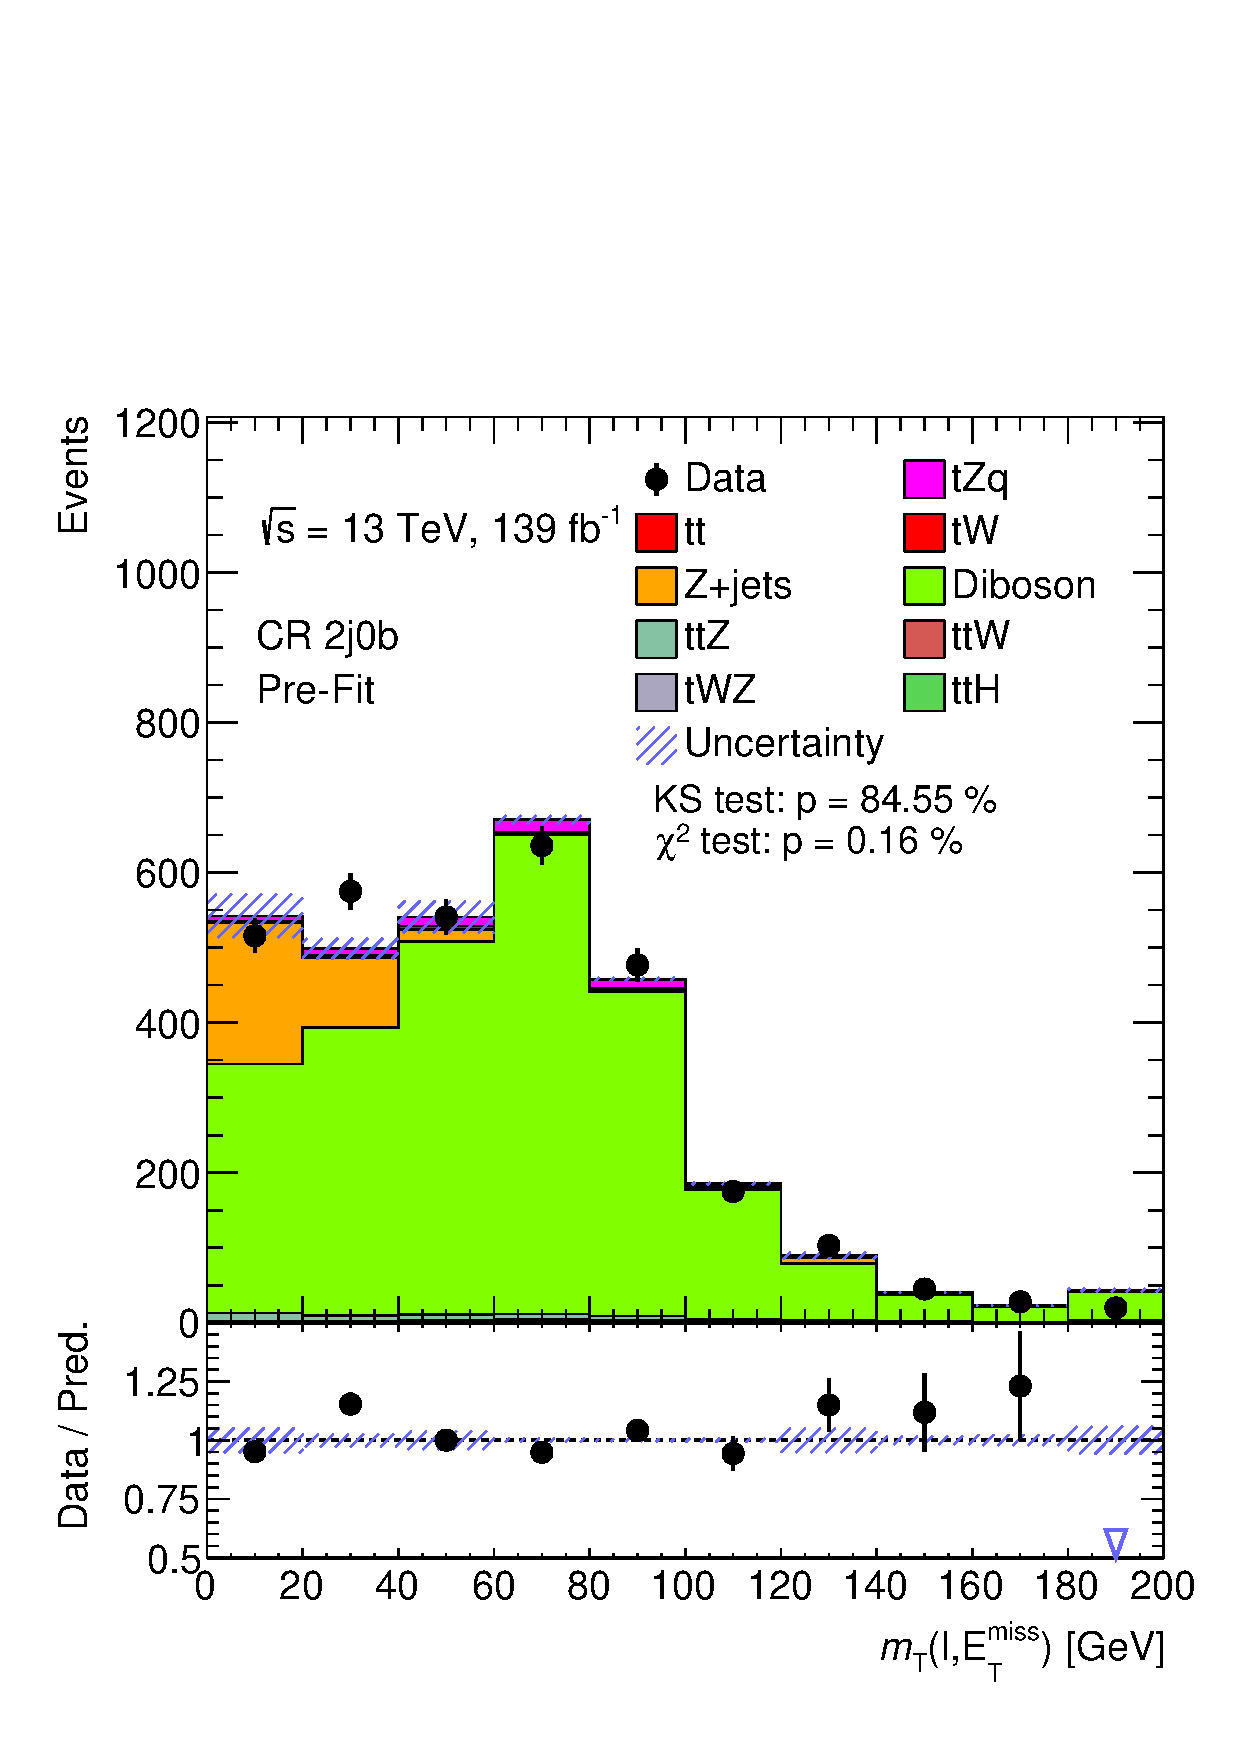
\includegraphics[width=\linewidth]{ubonn-thesis/Chapters/Chapters_05/Figure/CR_VV/CR_2j0b_mtW.pdf} 
  \end{subfigure} 
  \begin{subfigure}[b]{0.33\linewidth}
    \centering
    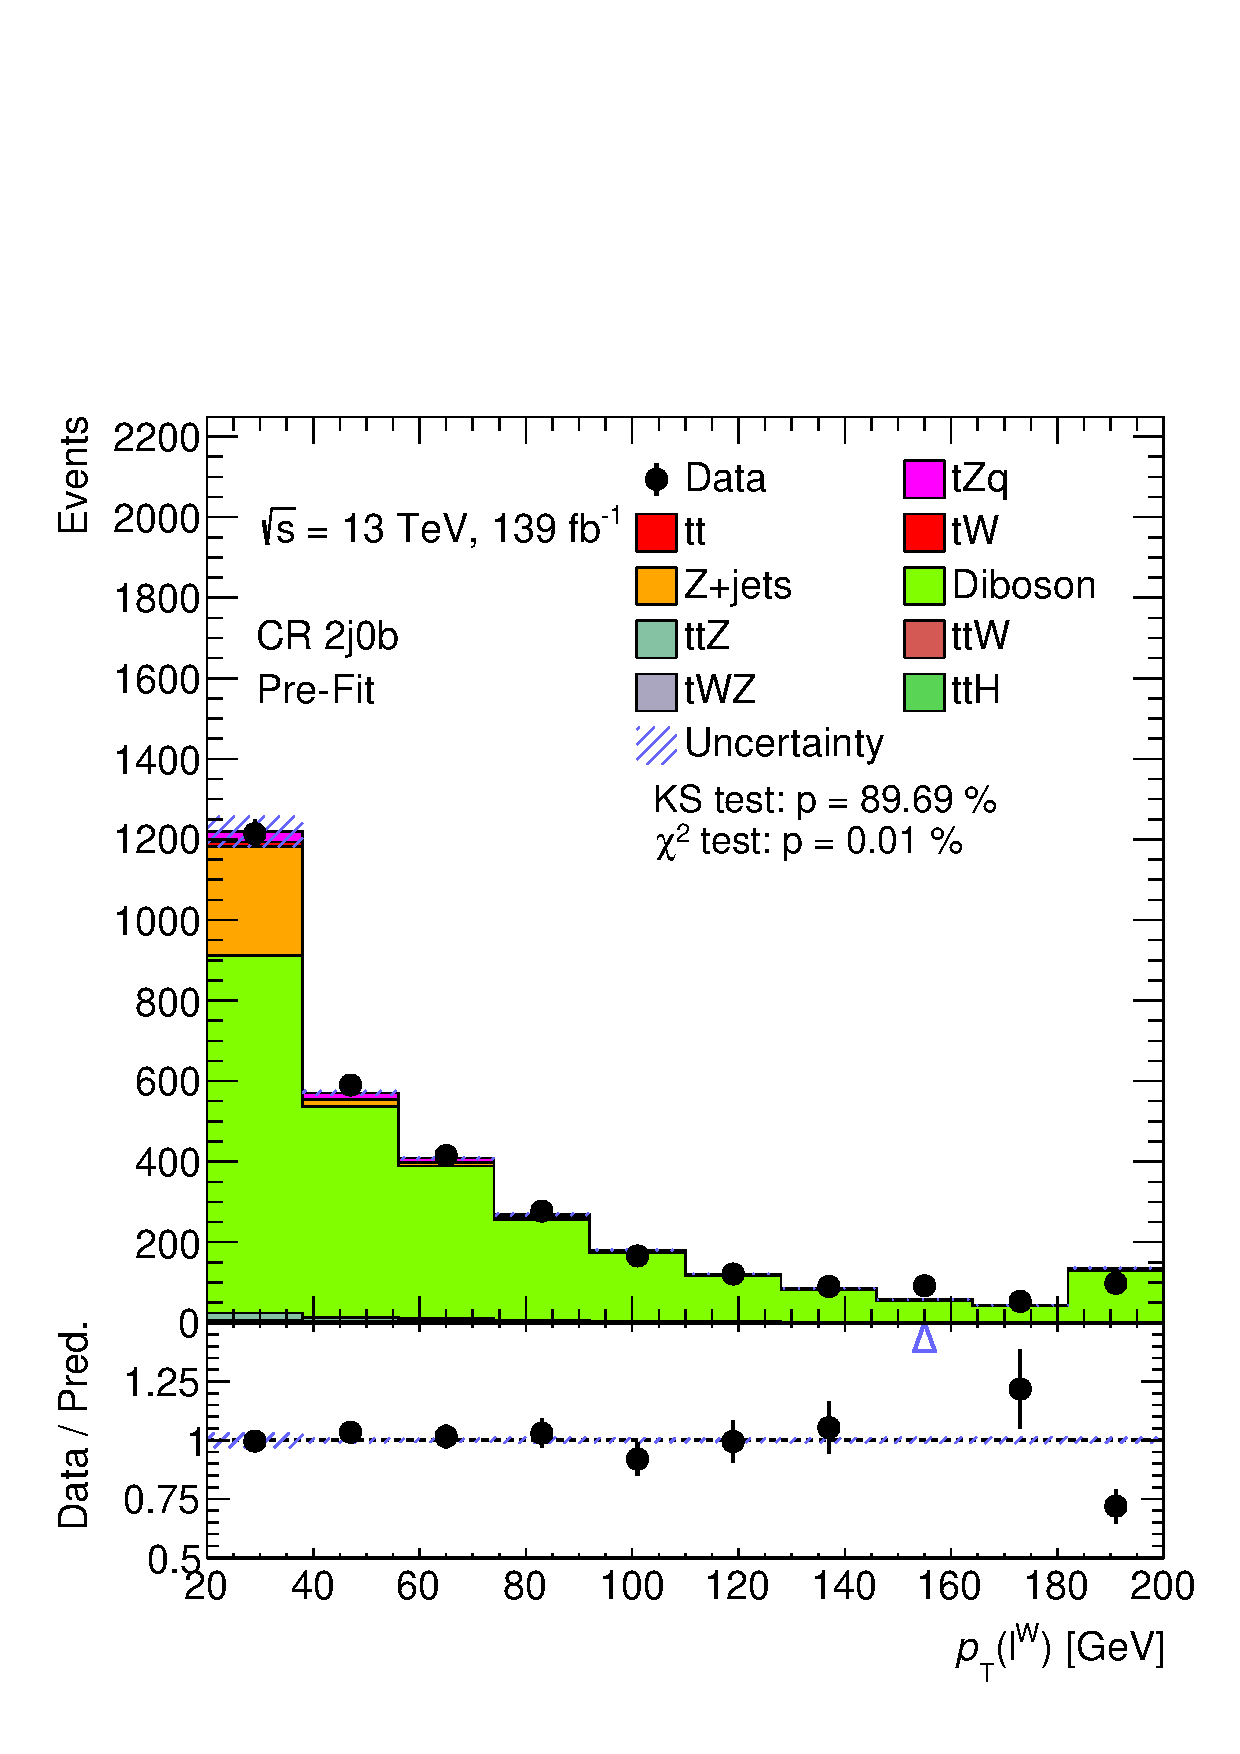
\includegraphics[width=\linewidth]{ubonn-thesis/Chapters/Chapters_05/Figure/CR_VV/CR_2j0b_lepW_pt.pdf} 
  \end{subfigure}%%
  \begin{subfigure}[b]{0.33\linewidth}
    \centering
    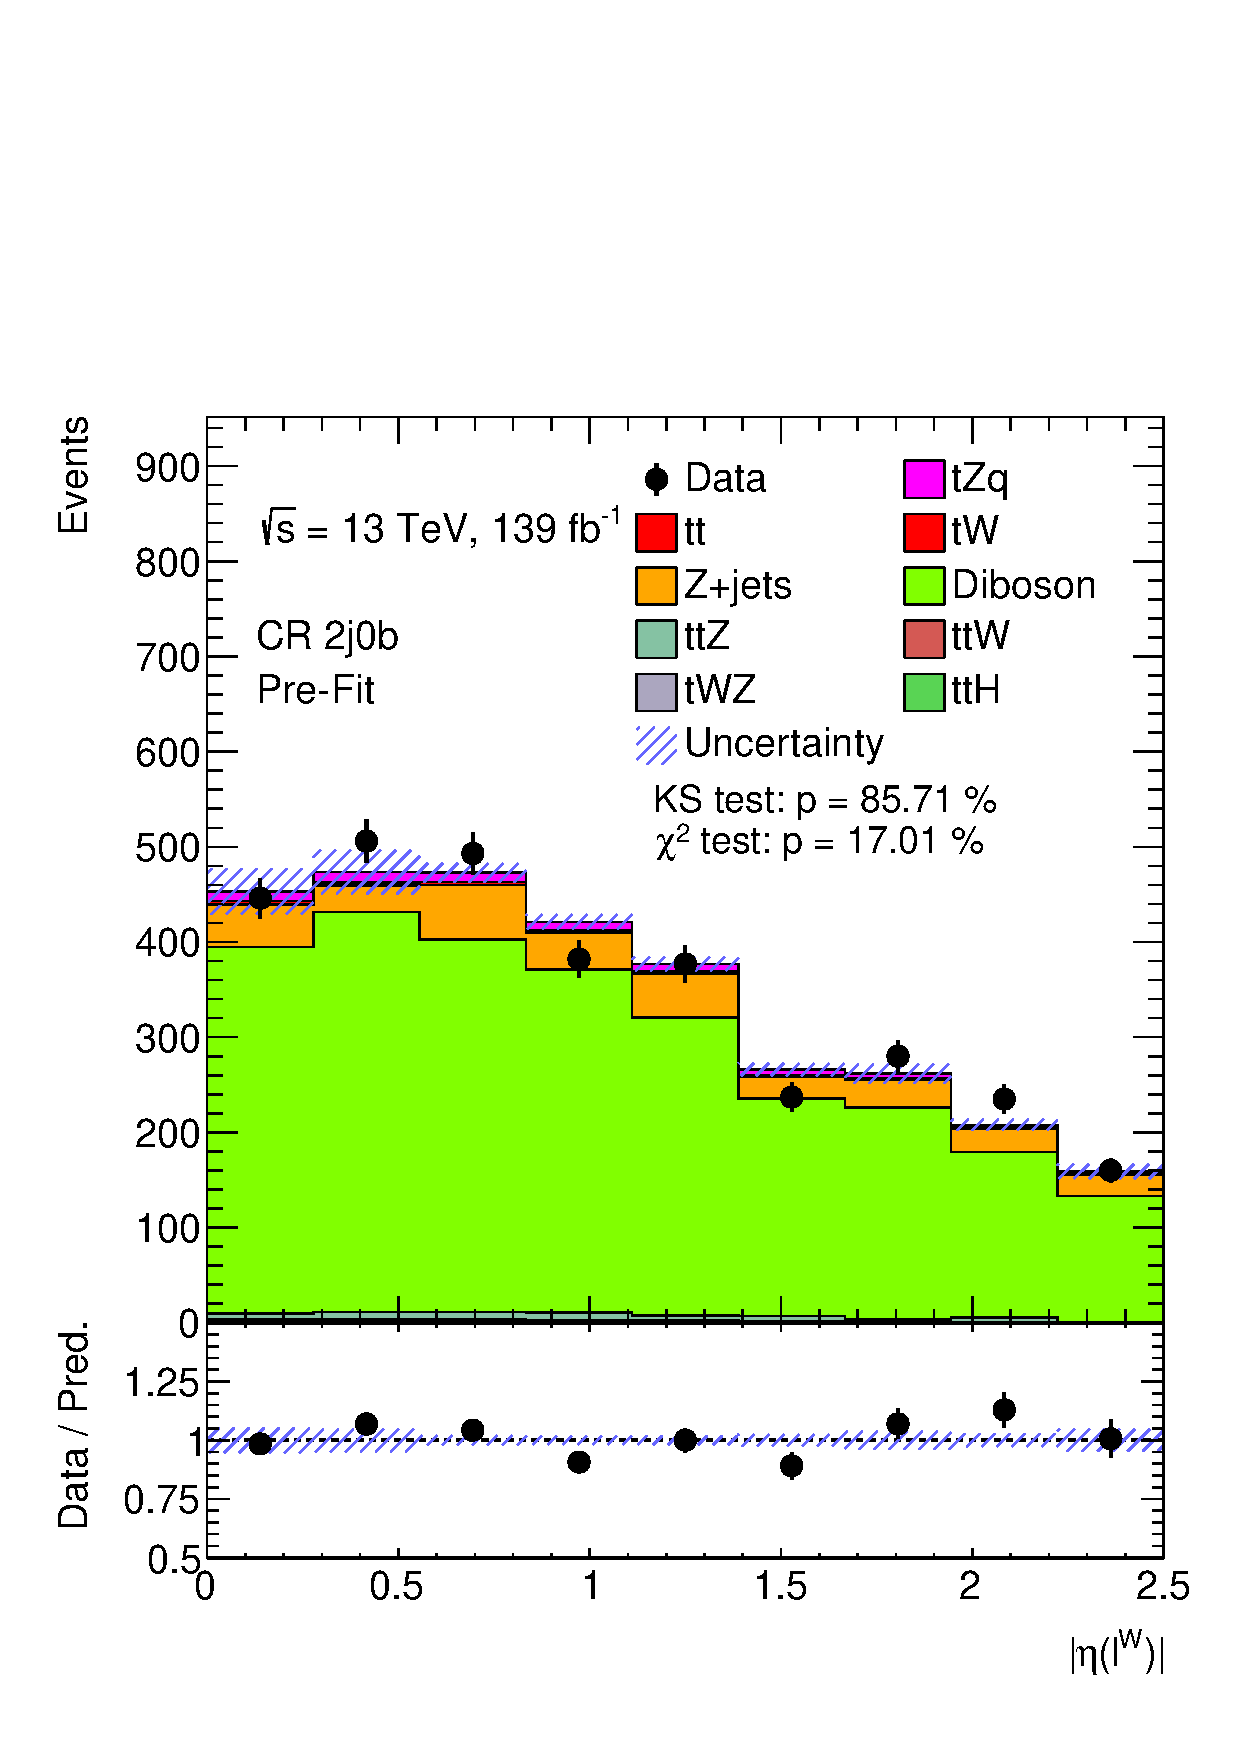
\includegraphics[width=\linewidth]{ubonn-thesis/Chapters/Chapters_05/Figure/CR_VV/CR_2j0b_lepW_eta.pdf} 
  \end{subfigure} 
  \newline
  \begin{subfigure}[b]{0.33\linewidth}
    \centering
    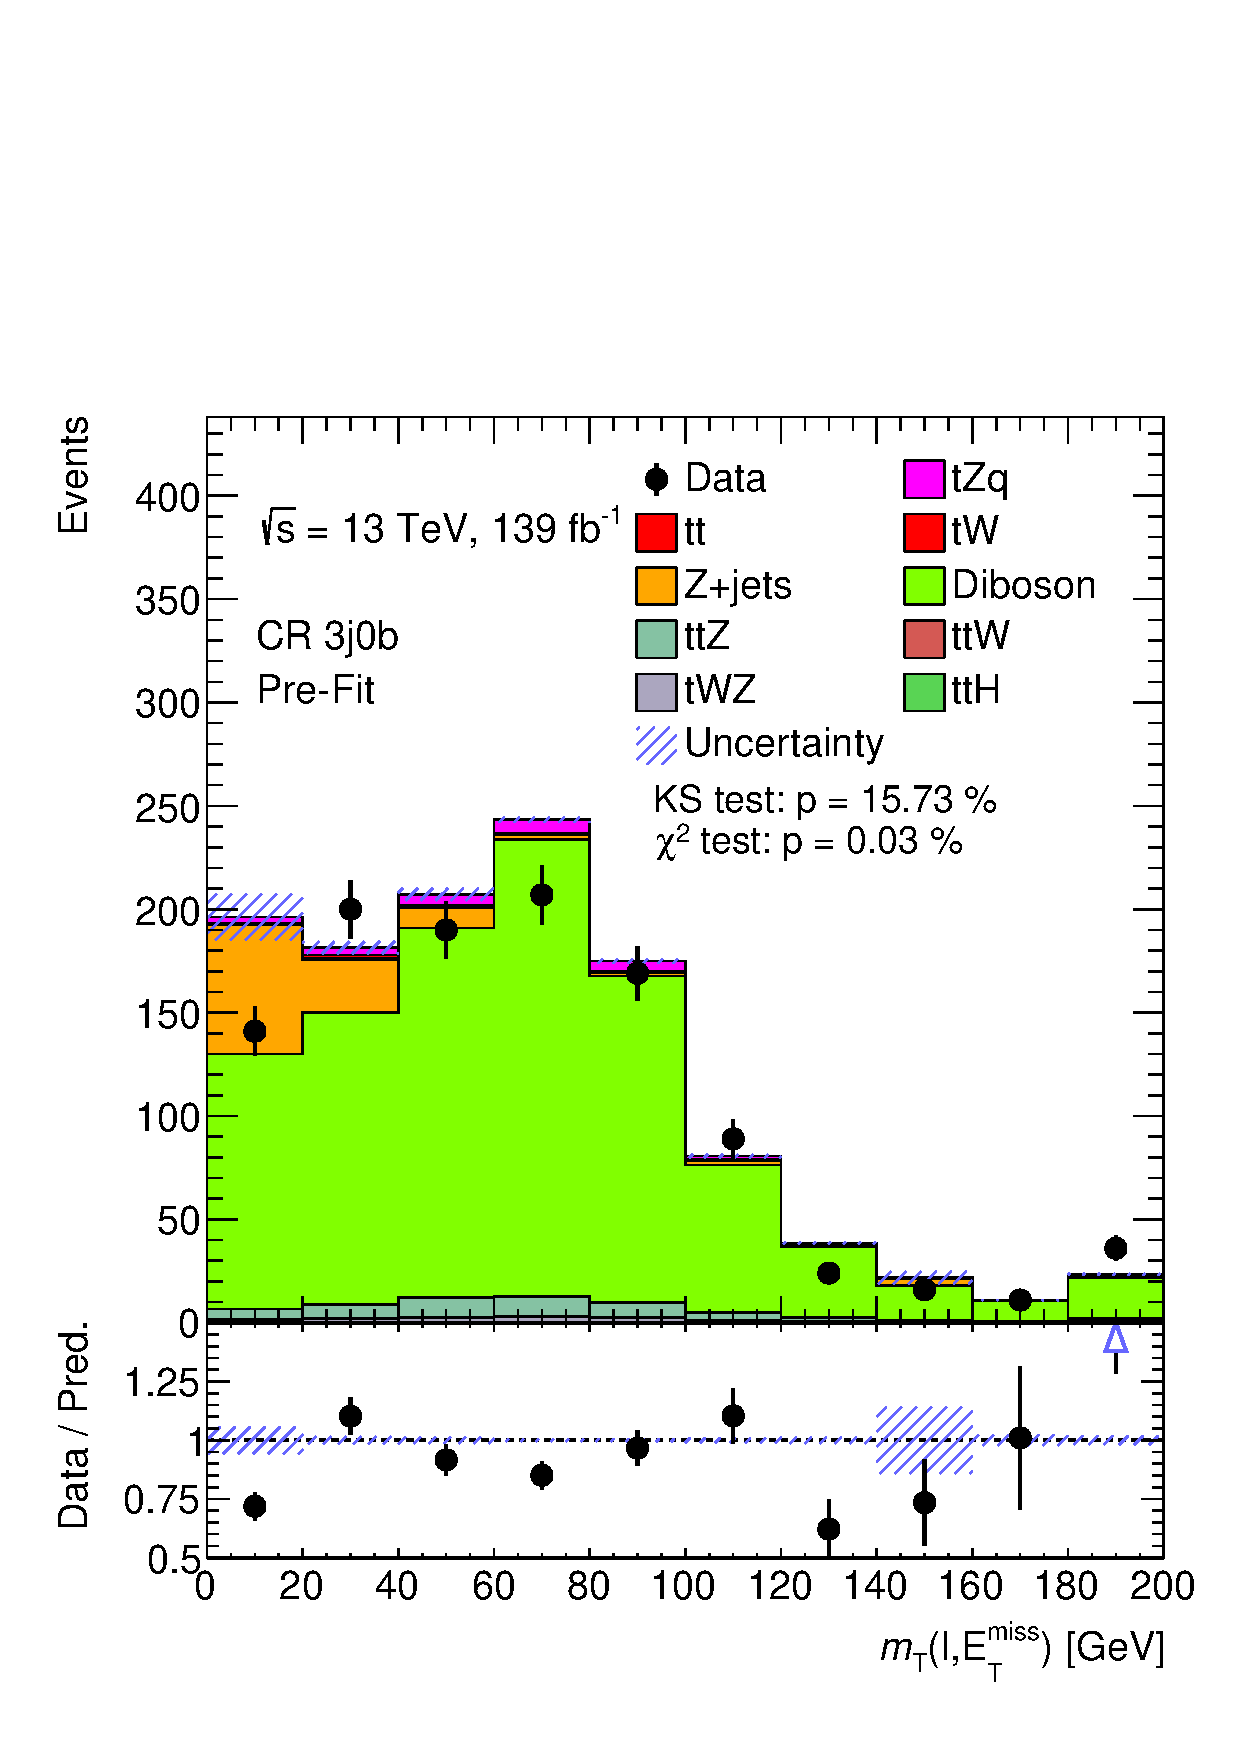
\includegraphics[width=\linewidth]{ubonn-thesis/Chapters/Chapters_05/Figure/CR_VV/CR_3j0b_mtW.pdf} 
  \end{subfigure} 
  \begin{subfigure}[b]{0.33\linewidth}
    \centering
    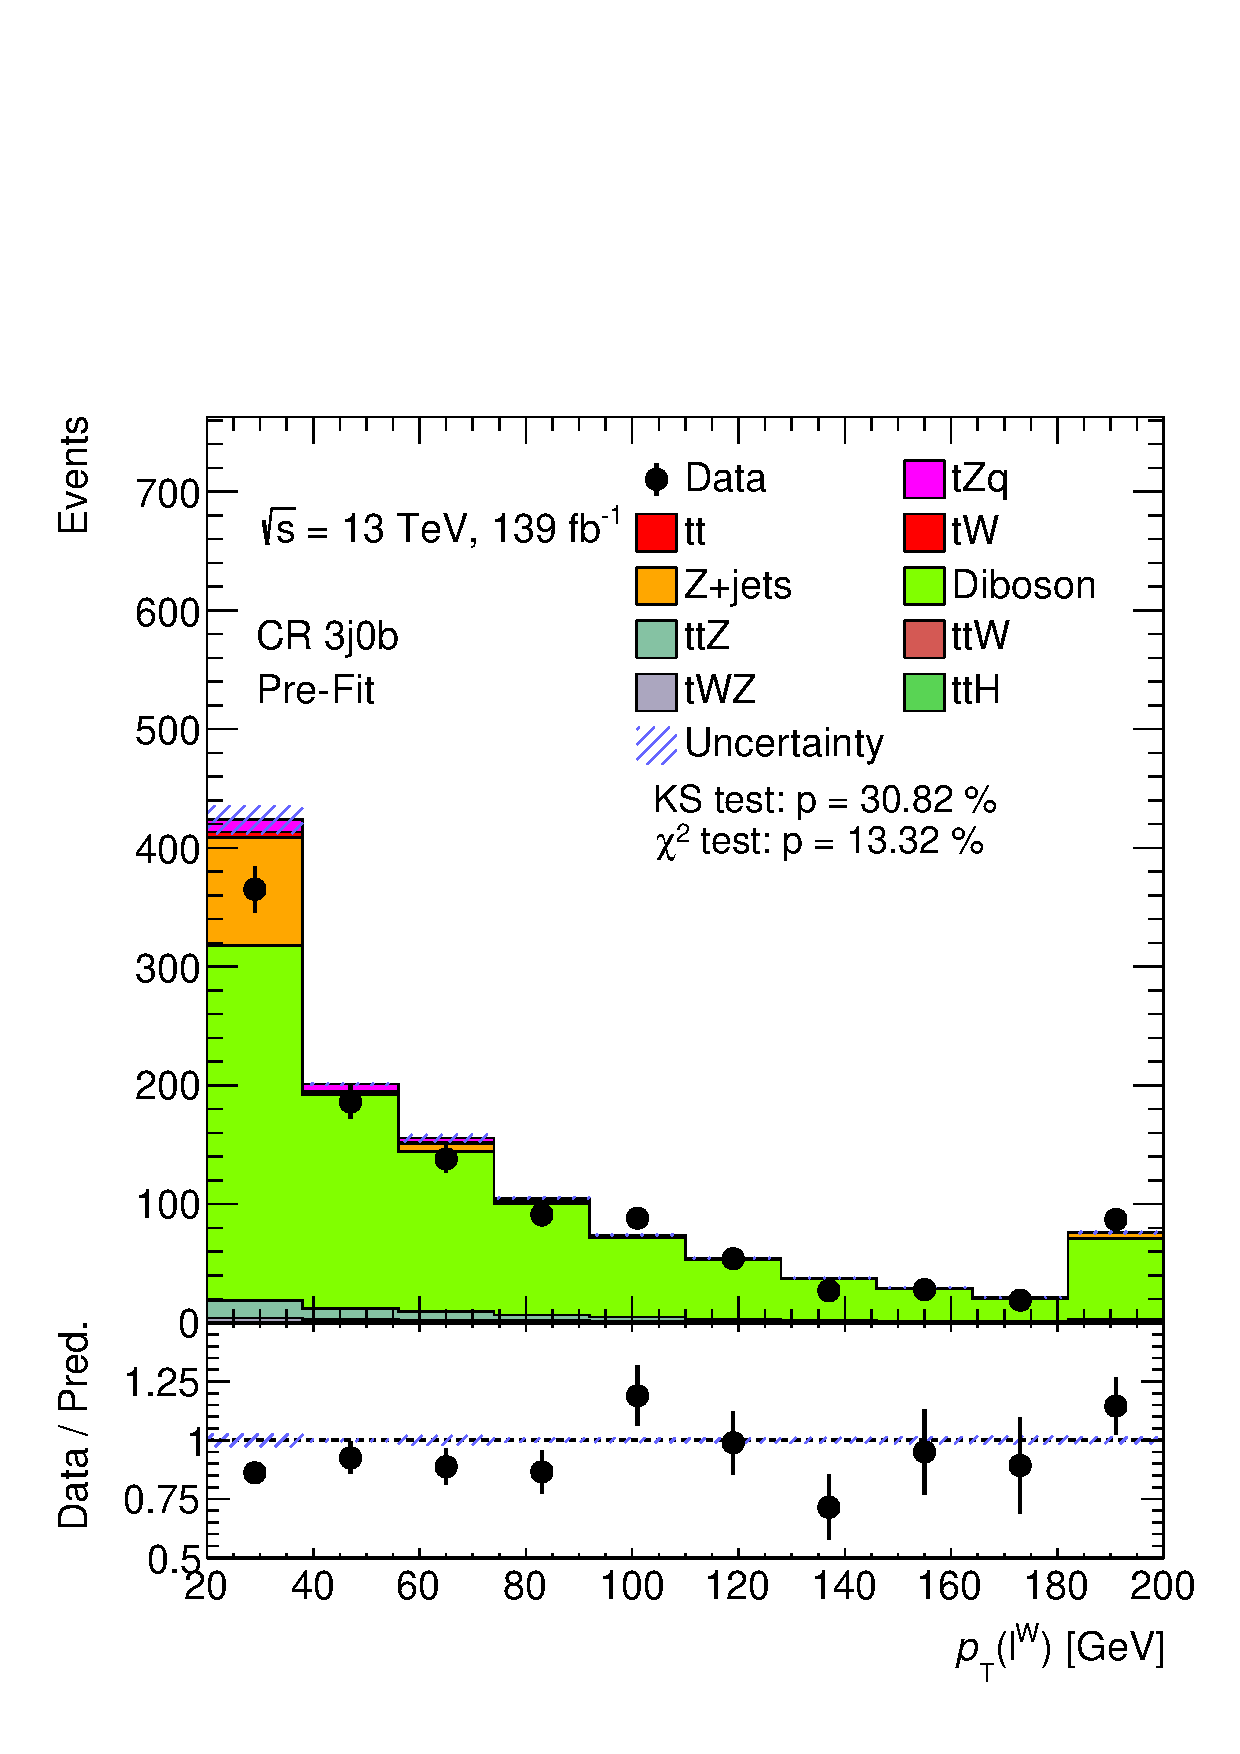
\includegraphics[width=\linewidth]{ubonn-thesis/Chapters/Chapters_05/Figure/CR_VV/CR_3j0b_lepW_pt.pdf} 
  \end{subfigure}%%
  \begin{subfigure}[b]{0.33\linewidth}
    \centering
    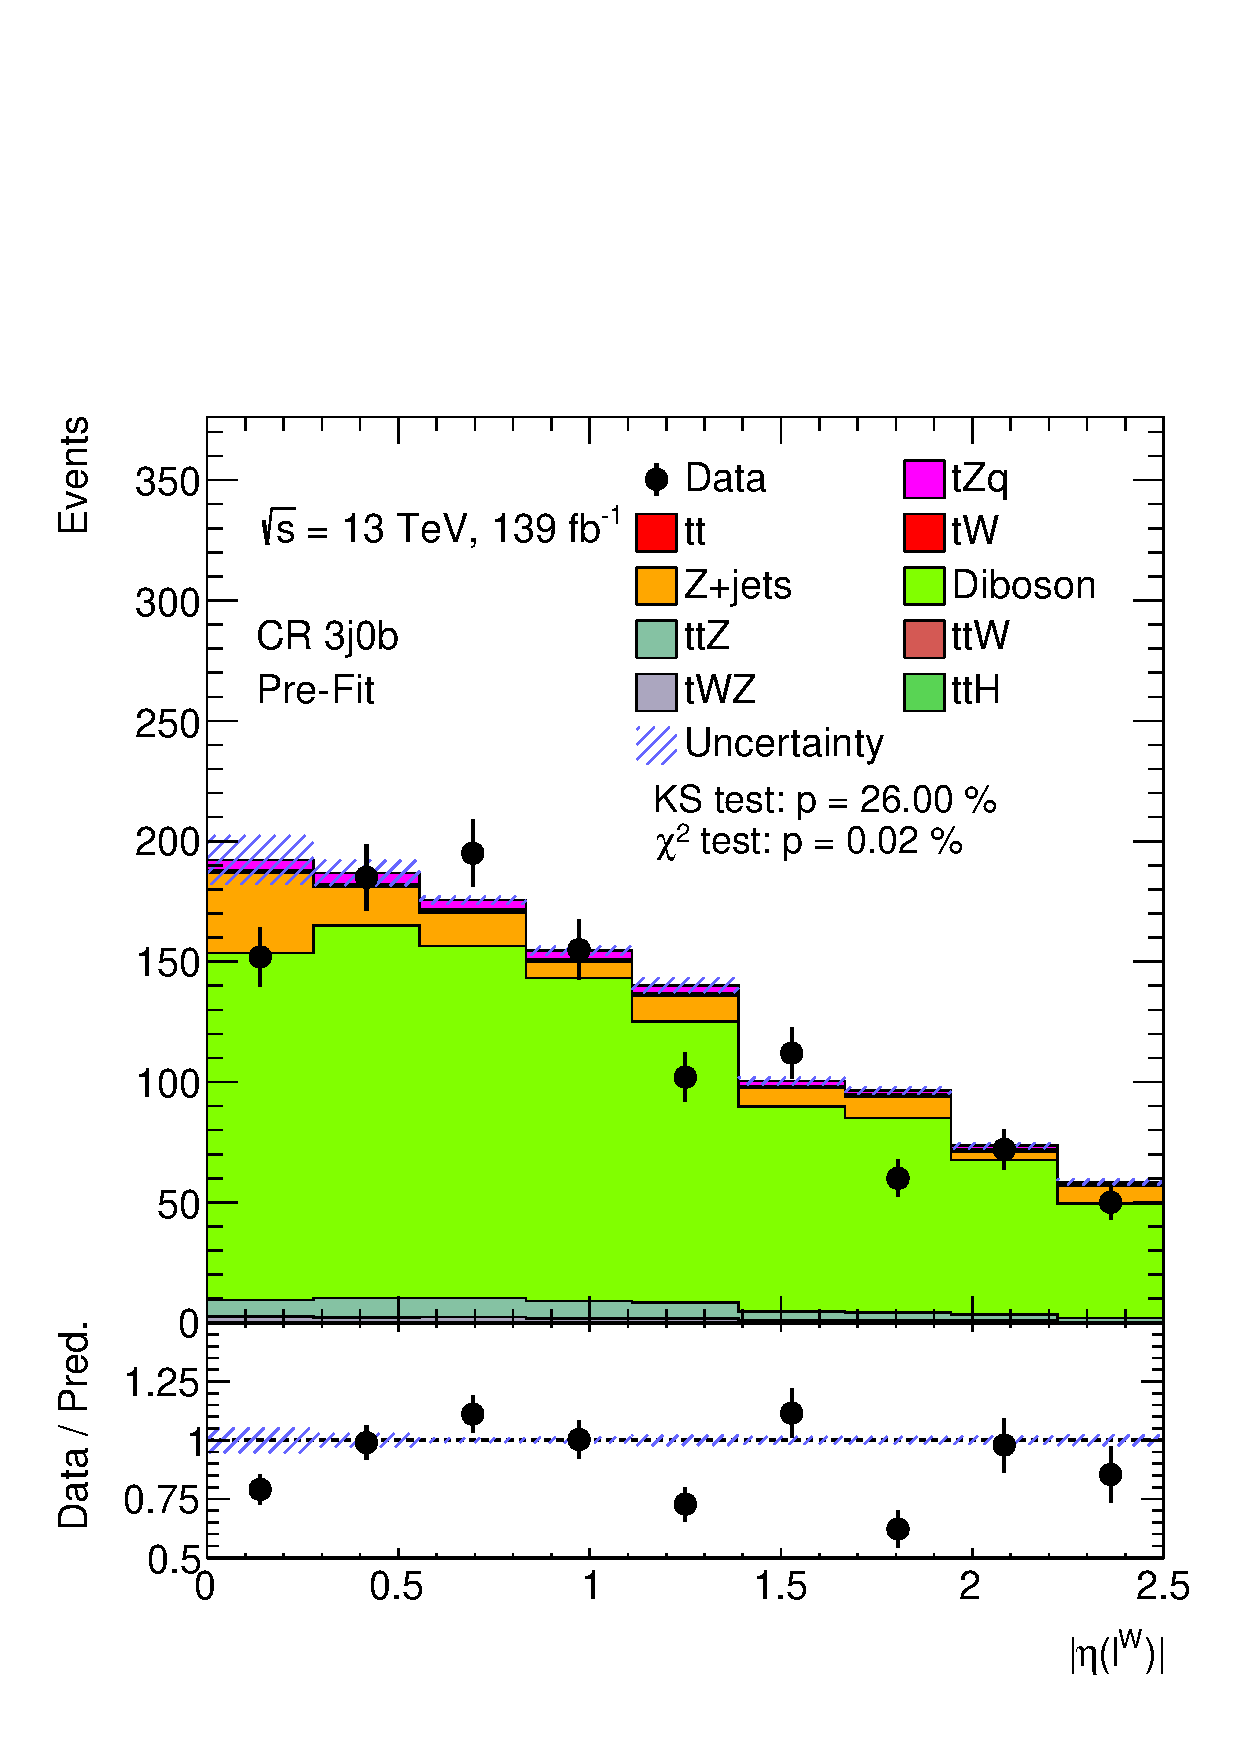
\includegraphics[width=\linewidth]{ubonn-thesis/Chapters/Chapters_05/Figure/CR_VV/CR_3j0b_lepW_eta.pdf} 
  \end{subfigure} 
  \caption{Comparison of data and MC predictions for reconstructed event related quantities for events in the CR 2j0b and CR 3j0b. }
  \label{fig:CRdibson}
  \end{figure}


 
The two diboson control regions are listed in table \ref{tab:final_selection}. The events yields in diboson CRs after the full section are shown in table \ref{tab:yield_diboson}. Some of the reconstructed variables in this control regions are shown in figure \ref{fig:CRdibson}.
The large number of observed events in this control region helps to provide a significant constraint on the overall rate of diboson events.  


\subsection{$t\Bar{t}Z$ CRs plots and yield}
\label{subsec:ttZ_plot_yield}


To define regions of phase space enriched in $t\Bar{t}Z$ production, an additional b-jet is required to enhance events with a second top quark. This region also contains significant amount of signal events. 

\vspace*{-0.4cm}
\begin{table}[!h]
    \begin{minipage}{.49\textwidth}
      \centering
      \begin{adjustbox}{width=\textwidth}
       \begin{tabular}{@{} *3l @{}}
 \toprule
 Process & Number of events & Number of raw events  \\ [0.5ex] 
 \hline\hline
  tZq   & 15.78 \pm 0.23 & 6584710\\ 
  tt   & 2.31 \pm 0.30 & 11120  \\ 
  tW   & 0.08 \pm 0.43   & 139 \\ 
  Z+jets   &  1.10 \pm 0.19 & 8062 \\ 
  Diboson   & 5.48 \pm 0.16  & 381555 \\ 
  ttZ   & 48.94 \pm 0.45 & 5681490 \\ 
  ttW   &  1.69 \pm 0.12 & 105501  \\ 
  tWZ   & 3.91 \pm 0.26 & 100775 \\ 
  ttH   & 1.59 \pm 0.04   & 488446 \\ 
\hline 
  Total expected  & 80.88 \pm 0.70 & 13361800  \\ 
\hline 
  Data   & 118  & 118  \\ 
 \bottomrule
 \end{tabular} 
 \end{adjustbox}
    \end{minipage}%
    \hfill
    \begin{minipage}{.49\textwidth}
      \centering
      \vspace*{0.5cm}
      \begin{adjustbox}{width=\textwidth}
        \begin{tabular}{@{} *3l @{}}
 \toprule
 Process & Number of events & Number of raw events  \\ [0.5ex] 
 \hline\hline
   tZq   & 10.43 \pm 0.20  & 5136470  \\ 
  tt   & 1.14 \pm 0.22 & 5699 \\ 
  tW   & 0.16 \pm 0.38 & 278  \\ 
  Z+jets & 0.56 \pm 0.13 & 4170 \\ 
  Diboson  & 3.38 \pm 0.12 & 230184 \\ 
  ttZ   & 53.35 \pm 0.51 & 7061060 \\ 
  ttW   & 0.76 \pm 0.07 & 42812  \\ 
  tWZ   & 4.76 \pm 0.29 & 120652  \\ 
  ttH   & 1.41 \pm 0.04  & 365153  \\ 
\hline 
  Total expected  & 75.94 \pm 0.68 & 12966500  \\ 
\hline 
  Data    & 77 & 77 \\  
 \bottomrule
 \end{tabular} 
 \end{adjustbox}
    \end{minipage} 
    \caption{Numbers of expected events in the CR 3j2b (Left) and CR 4j2b (Right) broken down by process. The uncertainty shown contains only the statistical component.}
    \label{tab:yield_ttZ}
\end{table}

\vspace*{-0.3cm}
\begin{figure}[h!] 
  \begin{subfigure}[b]{0.32\linewidth}
    \centering
    \includegraphics[width=\linewidth]{ubonn-thesis/Chapters/Chapters_05/Figure/CR_ttZ/CR_3j2b_Z_pt.pdf} 
  \end{subfigure}%% 
  \begin{subfigure}[b]{0.32\linewidth}
    \centering
    \includegraphics[width=\linewidth]{ubonn-thesis/Chapters/Chapters_05/Figure/CR_ttZ/CR_3j2b_Z_eta.pdf} 
  \end{subfigure} 
  \begin{subfigure}[b]{0.32\linewidth}
    \centering
    \includegraphics[width=\linewidth]{ubonn-thesis/Chapters/Chapters_05/Figure/CR_ttZ/CR_3j2b_Top_mass.pdf} 
  \end{subfigure}%%
  \newline
  \begin{subfigure}[b]{0.32\linewidth}
    \centering
    \includegraphics[width=\linewidth]{ubonn-thesis/Chapters/Chapters_05/Figure/CR_ttZ/CR_4j2b_Z_pt.pdf} 
  \end{subfigure} 
  \begin{subfigure}[b]{0.32\linewidth}
    \centering
    \includegraphics[width=\linewidth]{ubonn-thesis/Chapters/Chapters_05/Figure/CR_ttZ/CR_4j2b_Z_eta.pdf} 
  \end{subfigure}%% 
  \begin{subfigure}[b]{0.32\linewidth}
    \centering
    \includegraphics[width=\linewidth]{ubonn-thesis/Chapters/Chapters_05/Figure/CR_ttZ/CR_4j2b_Top_mass.pdf} 
  \end{subfigure}
  \caption{Comparison of data and MC predictions for reconstructed event- related quantities for events in the CR 3j2b and CR 4j2b. The uncertainty shown is the statistical uncertainty.}
  \label{fig:ttZ}
  \end{figure}



The two $t\Bar{t}Z$ control regions are listed in table \ref{tab:final_selection}. The events yields in $t\Bar{t}Z$ CRs after the full section are shown in table \ref{tab:yield_ttZ}. Some of the reconstructed variables in this control regions are shown in figure \ref{fig:ttZ}.

The $t\Bar{t}Z$ CRs are unique in that they require an extra b-jet which introduces an ambiguity in the event selection and reconstruction criteria. Here, only one of the b-jet is considered and other one is neglected. The forward jet is then selected as in section \ref{sec:SR}. The $t\Bar{t}Z$ CRs also have contamination from tZq signal events which can create a bias in the measurement. This is solved by fitting the neural-network output, $O_{NN}$ distribution (section \ref{sec:NN}) which shows seperation between the tZq and $t\Bar{t}Z$. This allows robust constraint of $t\Bar{t}Z$ modeling and also a slight boost to the overall measurement’s senstivity.


\subsection{$t\Bar{t}$ CRs plots and yields}
\label{subsec:tt_plot_yield}

Finally, the $t\Bar{t}$ contribution can be enhanced by requiring the OSSF lepton requirement be removed, effectively removing the requirement on the Z boson and opposite-sign, different-flavor (OSDF) leptons condition is imposed. This phase space is dominated by $t\Bar{t}$ events with a fake lepton and a b-jet. 

The two $t\Bar{t}$ CRs are also defined in table \ref{tab:final_selection}. The event yields in the $t\Bar{t}$ CRs after the full selection can be found in table \ref{tab:yield_ttbar} and reconstructed variables from the top quark and Z boson are given in figure \ref{fig:CR_tt}.

The $t\Bar{t}$ CRs suffer from the lowest statistics of all fitted regions. Because of this, two binned histograms per region is used in the statistical analysis.

\begin{table}[!h]
    \begin{minipage}{.49\textwidth}
      \centering
      \begin{adjustbox}{width=\textwidth}
       \begin{tabular}{@{} *3l @{}}
 \toprule
 Process & Number of events & Number of raw events  \\ [0.5ex] 
 \hline\hline
  tZq   &  0.34 \pm 0.04 & 200994 \\ 
  tt   &  43.40 \pm 1.23 & 197797 \\ 
  tW   & 2.32 \pm 0.52  & 3058 \\ 
  Z+jets   &  0.19 \pm 0.15 & 556  \\ 
  Diboson   & 0.39 \pm 0.07 & 21545 \\ 
  ttZ   & 2.69 \pm 0.12 & 262293 \\ 
  ttW   & 9.76 \pm 0.26 & 494284 \\ 
  tWZ   & 0.44 \pm 0.10  & 12649  \\ 
  ttH   &  3.35 \pm 0.05 & 1234180 \\ 
\hline 
  Total expected  & 62.87 \pm 1.37 & 2427360 \\ 
\hline 
  Data   & 71 & 71  \\ 
 \bottomrule
 \end{tabular} 
 \end{adjustbox}
    \end{minipage}%
    \hfill
    %\hspace{-1.5cm}
    \begin{minipage}{.50\textwidth}
      \centering
      \vspace*{0.5cm}
      \begin{adjustbox}{width=\textwidth}
        \begin{tabular}{@{} *3l @{}}
 \toprule
 Process & Number of events & Number of raw events  \\ [0.5ex] 
 \hline\hline
   tZq   & 0.21 \pm 0.03  & 139834  \\ 
  tt   & 20.27 \pm 0.84 &  93408 \\ 
  tW   & 1.06 \pm 0.61  & 1251 \\ 
  Z+jets & 0.13 \pm 0.13 &  417 \\ 
  Diboson  & 0.30 \pm 0.04 & 14178 \\ 
  ttZ   & 2.47 \pm 0.12 & 284950  \\ 
  ttW   & 5.19 \pm 0.20 & 308302  \\ 
  tWZ   & 0.26 \pm 0.09 & 10981 \\ 
  ttH   & 3.90 \pm 0.06  &  1.222370 \\ 
\hline 
  Total expected  & 33.80 \pm 0.96   & 2075690  \\ 
\hline 
  Data    & 49 & 49 \\ 
 \bottomrule
 \end{tabular} 
 \end{adjustbox}
    \end{minipage} 
    \caption{Numbers of expected events in the CR 2j1b (Left) and CR 3j1b (Right) broken down by process. The uncertainty shown contains only the statistical component.}
    \label{tab:yield_ttbar}
\end{table}


\begin{figure}[h!] 
  \begin{subfigure}[b]{0.33\linewidth}
    \centering
    \includegraphics[width=\linewidth]{ubonn-thesis/Chapters/Chapters_05/Figure/CR_tt/CR_2j1b_M_bj.pdf} 
  \end{subfigure}%% 
  \begin{subfigure}[b]{0.33\linewidth}
    \centering
    \includegraphics[width=\linewidth]{ubonn-thesis/Chapters/Chapters_05/Figure/CR_tt/CR_2j1b_forwardjet_eta.pdf} 
  \end{subfigure} 
  \begin{subfigure}[b]{0.33\linewidth}
    \centering
    \includegraphics[width=\linewidth]{ubonn-thesis/Chapters/Chapters_05/Figure/CR_tt/CR_3j1b_M_bj.pdf} 
  \end{subfigure}%%
  \newline
  \begin{subfigure}[b]{0.33\linewidth}
    \centering
    \includegraphics[width=\linewidth]{ubonn-thesis/Chapters/Chapters_05/Figure/CR_tt/CR_2j1b_M_bj.pdf} 
  \end{subfigure}%% 
  \begin{subfigure}[b]{0.33\linewidth}
    \centering
    \includegraphics[width=\linewidth]{ubonn-thesis/Chapters/Chapters_05/Figure/CR_tt/CR_2j1b_forwardjet_eta.pdf} 
  \end{subfigure} 
  \begin{subfigure}[b]{0.33\linewidth}
    \centering
    \includegraphics[width=\linewidth]{ubonn-thesis/Chapters/Chapters_05/Figure/CR_tt/CR_3j1b_M_bj.pdf} 
  \end{subfigure}%%
  \caption{Comparison of data and MC predictions for reconstructed event- related quantities for events in the CR 2j1b and CR 3j1b. The uncertainty shown is the statistical uncertainty.}
  \label{fig:CR_tt} 
  \end{figure}
  

%\begin{figure}[ht!] 
  
%\end{figure}


% !TEX root = mythesis.tex

%==============================================================================
\chapter{Analysis}
\label{chap:multivariate_analysis}

This chapter describes the setup that will be used in the final fit to the data and the expected signal and background events described in chapter \ref{chap:data_MC}. 

Section \ref{sec:strategy} gives an overview of the fit used for extracting a cross-section measurement. Section \ref{sec:NN} presents the signal and background separation procedure, where an artificial neural network is used as multivariate classification technique.  Section \ref{sec: Profile_likehihood} gives a basic idea of binned profile likelihood fit which is used is used for signal extraction in this thesis. Section \ref{sec:systematics} explains in short about the systematic uncertainties that can modify the rate of the signal and background process. Section \ref{subsec:fittedregions} gives an overview of the fitted regions along with corresponding distributions. Finally, binning optimisation is presented in section \ref{subsec:binningoptimization}. 

%==============================================================================
\section{Cross-section measurement analysis strategy}
\label{sec:strategy}

The strategy of this analysis is to determine the signal strength $\mu_{tZq}$ (POI) of the tZq process, hence the total cross-section while including systematic uncertainties as nuisance parameter in the profile likelihood fit as described in section \ref{sec: Profile_likehihood}. Two different signal regions as defined in section \ref{sec:SR}, with different amount of signal and background contributions, are used to determine $\mu_{tZq}$. As defined in section \ref{sec:CR}, control regions are defined  to determine the normalization of the respective dominant background processes. Both the signal and three backgrounds, $t\Bar{t}$ + tW and Z+jets , \& $t\Bar{t}Z$ normalization factors are fitted as free parameters in all eight regions simultaneously. The contributions of all other backgrounds are set to their expected values and are allowed to vary within their systematic uncertainties, which are included as nuisance parameter in the fit. For the cross-section of tZq, where the Z boson decays into the charged leptons ($e^{+}e^{-}$, $\mu^{+}\mu^{-}$), $\sigma_{tl^{+}l^{-}q}$ = 102 fb is assumed to be the nominal value \cite{tZq2020} for the fit. which corresponds to the signal strength of $\mu = 1$.


\section{Multivariate analysis technique: Artificial Neural Network (NN)}
\label{sec:NN}
In order to separate the signal and background for the SM tZq processes, a cut-and-count analysis is difficult and will give bad sensitivity, due to the large number of background events and the big uncertainties associated to them. In high energy physics,  multivariate analysis techniques such artificial neural networks (NN's) have been used or proposed as good candidates for tasks of signal versus background classification.

\begin{figure}[h!] 
  \begin{subfigure}[b]{0.49\linewidth}
    \centering
    \includegraphics[width=\textwidth]{ubonn-thesis/Chapters/Chapters_06/Figure/Neural Network/SR_2j1b_correlation.pdf}
    \caption{}
    \end{subfigure}%% 
  \begin{subfigure}[b]{0.5\linewidth}
    \centering
    \includegraphics[width=0.6\linewidth]{ubonn-thesis/Chapters/Chapters_06/Figure/Neural Network/neural_network.pdf} 
    \caption{}
    \label{NN_config}
  \end{subfigure}
  \caption{ a) Correlation matrix between the input variables used for training in the SR 2j1b . b) Neural network configuration used for training. It is drawn using tikZ package in latex. Meaning of variables and numbers given in table \ref{tab:NN_input}}
  \label{fig:NN_configuration}
  \end{figure}


An artificial neural network (NN) is a simplified mathematical structure inspired from the real biological neural networks. It has similar basic concepts of a real biological neural network (neuron, connection strength, input linearity, output-linearity) but in a much more conservative level of complexity. The neuron is a mathematical entity which has a real value depending on the connection strengths (weights) and the values of the other neurons with which it is connected. The non-linear function that relates the output from the neuron with the weights and the inputs to the neuron is usually called \textit{activation function}. A neural network can be structured as layers. The input layer, from where the NN is fed with the input variables of the problem to be solved, followed by a number of layers called hidden layers, and finally the output layers.


An example of a multi-layer neural network is shown in figure \ref{NN_config}. Let us consider a multi-layer neural network having a layer of n input neurons $X_{i}$ (i=1,\dots,n), with an activation function $f_{X_{i}}$, a hidden layer of m neurons $H_{j}$ (j=1,\dots,m) with activation function $f_{H_{j}}$and an output layer of two neurons $Y_{p}$ (p=1,2) with activation function $f_{Y_{p}}$. The output node gives continuous output ($O_{NN}$) between 0 and 1, where the output tends to 0 for background, and +1 for signal. The neural network output is calculated as follows:

\begin{equation}
    \label{eqn:NNout}
     Y_{p} = f_{Y_{p}}(\zeta_{Y_{p}}) = f_{Y_{p}}\left( \sum_{j=1}^{m+1} w_{pj}f_{H_{j}}(\zeta_{H_{j}}) \right) = f_{Y_{p}}\left( \sum_{j=1}^{m+1} w_{pj}f_{H_{j}}\left( \sum_{i=1}^{n+1} v_{ji}f_{X_{i}}(X_{i}) \right) \right)
\end{equation}

where $w_{pj}$ are the weights between the input layer and the hidden layer, and $v_{ji}$ are the weights between the hidden layer and the output layer.

In this analysis a supervised neural network with three-layer feed-forward algorithm is implemented using Tensflow in Python \cite{tensorflow_developers_2021_5799851}.  Elu is used as activation function for both input and hidden layers whereas sigmoid for output layer. The response curve for various activation functions including elu and sigmoid can be seen in ref. \cite{nwankpa2018activation}.



\subsection{Input variables}
The input variables are chosen in an iterative process. First, many variables are used to train preliminary NN. The correlations between variables in MC events are determined. In the second step, the relevant variables with the biggest separation power are investigated by comparing the MC distributions. The signal event signature is simple as defined in section \ref{sec:SR}. Thus, the input variables are limited and can be categorized as: variables measured directly in the detector, others which are reconstructed from the measured quantities as described in section \ref{sec:event_reconstruction}. All possible variables such as momenta, relative angles, pseudo-rapidity, and particle masses are explored. The  variables used to train the NN in the SR 2j1b, SR 3j1b, CR 3j2b, and CR 4j2b are listed with their rank in table \ref{tab:NN_input}. The ranking of variables is done by comparing the statistics value obtained after training the NN with and without the variable. So, the training is repeated as many times as there are variables in list. The statistics is obtained by performing the t-test of the output of NN for the two cases. 

\begin{table}[h!]
\centering
\begin{adjustbox}{width=\textwidth}
\begin{tabular}{@{} *4l  @{}}
\toprule
Variable & \multicolumn{2}{c}{Rank} & Definition \\
 & SR 2j1b & SR 3j1b &  \\
 \midrule
 $m_{bj_{f}}$ & 1 & 1 & (Largest) invariant mass of the b-jet and the untagged jet(s) \\[0.2ex]
 $m_{t}$   &  2 &  2 & Reconstructed top-quark mass \\[0.2ex]
 $p_{T}(W)$     &  3 & 3 & $p_{T}$ of the reconstructed W boson \\[0.2ex]
 $p_{T}(Z)$    & 4 &  4 & $p_{T}$ of the reconstructed Z boson \\[0.2ex]
 $p_{T}(j_{f})$    & 5 & 5 & $p_{T}$ of the forward jet\\[0.2ex]
 $p_{T}(\ell_{W})$ & 6 & 7 & $p_{T}$ of the lepton from the W-boson decay\\[0.2ex]
 $m_{Z}$   & 7 & 8 & Mass of the reconstructed Z boson\\[0.2ex]
 $m_{T}(\ell,E_{T}^{miss})$ &  8 &  9 & Transverse mass of the W boson \\[0.2ex]
 $|\eta(\ell_{W})|$ &  9 & 10 & Absolute value of the $\eta$ of the lepton from the W boson decay\\[0.2ex]
 $|\eta(j_{f})|$  &  10 &  12 & Absolute value of the $\eta$ of the forward jet\\[0.2ex]
$\Delta R(j_{f},Z)$ & 11 &  14 &  $\Delta R$ between the forward jet and the reconstructed Z boson \\[0.2ex]
b-tagging score   &  12 & 15 & b-tagging score of the b-jet \\[0.2ex]
$|\eta(Z)|$  & 13 & 13 & Absolute value of the $\eta$ of the reconstructed Z boson \\[0.2ex]
$E_{T}^{miss}$ & 14 & 16 & Missing transverse momentum \\[0.2ex]
$p_{T}(j_{r})$  &{--}& 6  & $p_{T}$ of the radiation jet \\[0.2ex]
$|\eta(j_{r})|$     & {--} &  11 & Absolute value of the $\eta$ of the $j_{r}$ jet \\[0.2ex]
\bottomrule
\end{tabular}
\end{adjustbox}
\caption{Variables used as input to the neural network in SR 2j1b and SR 3j1b. The ranking of the variables in each of the SRs is given in the 2nd and 3rd columns, respectively.}
\label{tab:NN_input}
\end{table}  


\subsection{Data and MC comparison}

Since the neural network is trained with simulated events, it is important to check if the input variables
are modelled correctly. Data and MC distributions are compared in figures \ref{fig_signal1}, \ref{fig_signal2}, \ref{fig_signal3}, \ref{fig_signal4} and \ref{fig_signal5}. All MC distributions are normalised using their predicted cross-section values. Kolmogorov-Smirnov test (KS-test) and Chi-Square ($\chi^{2}$-test) are performed for each distributions. The p-value obtained during the test is shown along with the distributions. Technically, KS-test is used to decide if a sample comes from a population with a specific distribution. 

\begin{figure}[!h] 
  \begin{subfigure}[b]{0.33\linewidth}
    \centering
    \includegraphics[width=\linewidth]{ubonn-thesis/Chapters/Chapters_06/Figure/Input_distribution/SR_2j1b_M_bj.pdf} 
  \end{subfigure}%% 
  \begin{subfigure}[b]{0.33\linewidth}
    \centering
    \includegraphics[width=\linewidth]{ubonn-thesis/Chapters/Chapters_06/Figure/Input_distribution/SR_2j1b_Top_mass.pdf} 
  \end{subfigure} 
  \begin{subfigure}[b]{0.33\linewidth}
    \centering
    \includegraphics[width=\linewidth]{ubonn-thesis/Chapters/Chapters_06/Figure/Input_distribution/SR_2j1b_W_pt.pdf} 
  \end{subfigure}%%
  \newline
  \begin{subfigure}[b]{0.33\linewidth}
    \centering
    \includegraphics[width=\linewidth]{ubonn-thesis/Chapters/Chapters_06/Figure/Input_distribution/SR_2j1b_Z_pt.pdf} 
  \end{subfigure} 
  \begin{subfigure}[b]{0.33\linewidth}
    \centering
    \includegraphics[width=\linewidth]{ubonn-thesis/Chapters/Chapters_06/Figure/Input_distribution/SR_2j1b_forwardjet_pt.pdf} 
  \end{subfigure}%% 
  \begin{subfigure}[b]{0.33\linewidth}
    \centering
    \includegraphics[width=\linewidth]{ubonn-thesis/Chapters/Chapters_06/Figure/Input_distribution/SR_3j1b_lepW_pt.pdf} 
  \end{subfigure} 
  \newline
  \begin{subfigure}[b]{0.33\linewidth}
    \centering
    \includegraphics[width=\linewidth]{ubonn-thesis/Chapters/Chapters_06/Figure/Input_distribution/SR_2j1b_MZ.pdf} 
  \end{subfigure}%%
  \begin{subfigure}[b]{0.33\linewidth}
    \centering
    \includegraphics[width=\linewidth]{ubonn-thesis/Chapters/Chapters_06/Figure/Input_distribution/SR_2j1b_mtW.pdf} 
  \end{subfigure}
  \begin{subfigure}[b]{0.33\linewidth}
    \centering
    \includegraphics[width=\linewidth]{ubonn-thesis/Chapters/Chapters_06/Figure/Input_distribution/SR_2j1b_lepW_eta.pdf} 
  \end{subfigure} 
  
  \caption{ Stacked kinematic plots of neural-network training variables of the SR 2j1b, in order of significance. Both signal and backgrounds are normalised to the expected number of events before the fit. The uncertainty band includes statistical uncertainties for signal and backgrounds }
  \label{fig_signal1} 
  \end{figure}


\begin{figure}
    \begin{subfigure}[b]{0.32\linewidth}
    \centering
    \includegraphics[width=\linewidth]{ubonn-thesis/Chapters/Chapters_06/Figure/Input_distribution/SR_2j1b_forwardjet_eta.pdf} 
  \end{subfigure}%%
  \begin{subfigure}[b]{0.32\linewidth}
    \centering
    \includegraphics[width=\linewidth]{ubonn-thesis/Chapters/Chapters_06/Figure/Input_distribution/SR_2j1b_dR_jf_Z.pdf} 
  \end{subfigure}
  \begin{subfigure}[b]{0.32\linewidth}
    \centering
    \includegraphics[width=\linewidth]{ubonn-thesis/Chapters/Chapters_06/Figure/Input_distribution/SR_2j1b_btag.pdf} 
  \end{subfigure} 
  \newline
  \centering
  \begin{subfigure}[b]{0.32\linewidth}
    \includegraphics[width=\linewidth]{ubonn-thesis/Chapters/Chapters_06/Figure/Input_distribution/SR_2j1b_Z_eta.pdf} 
  \end{subfigure}%% 
  \hspace*{0.3cm}
  \centering
  \begin{subfigure}[b]{0.32\linewidth}
    \includegraphics[width=\linewidth]{ubonn-thesis/Chapters/Chapters_06/Figure/Input_distribution/SR_2j1b_MissEt.pdf} 
  \end{subfigure} 
  \caption{Stacked kinematic plots of neural-network training variables of the SR 2j1b, in order of significance. Both signal and backgrounds are normalised to the expected number of events before the fit. The uncertainty band includes statistical uncertainties for signal and backgrounds}
  \label{fig_signal2} 
\end{figure}
%% delta R and pt of forward jet

%% SR 3j1b
\begin{figure}[!h] 
  \begin{subfigure}[b]{0.32\linewidth}
    \centering
    \includegraphics[width=\linewidth]{ubonn-thesis/Chapters/Chapters_06/Figure/Input_distribution/SR_3j1b_M_bj.pdf} 
  \end{subfigure}%% 
  \begin{subfigure}[b]{0.32\linewidth}
    \centering
    \includegraphics[width=\linewidth]{ubonn-thesis/Chapters/Chapters_06/Figure/Input_distribution/SR_3j1b_Top_mass.pdf} 
  \end{subfigure} 
  \begin{subfigure}[b]{0.32\linewidth}
    \centering
    \includegraphics[width=\linewidth]{ubonn-thesis/Chapters/Chapters_06/Figure/Input_distribution/SR_3j1b_W_pt.pdf} 
  \end{subfigure}%%
  \caption{Stacked kinematic plots of neural-network training variables of the SR 3j1b, in order of significance. Both signal and backgrounds are normalised to the expected number of events before the fit. The uncertainty band includes statistical uncertainties for signal and backgrounds}
  \label{fig_signal3}
  \end{figure}


\begin{figure}[!h] 
\vspace*{0.4cm}
  \begin{subfigure}[b]{0.33\linewidth}
    \centering
    \includegraphics[width=\linewidth]{ubonn-thesis/Chapters/Chapters_06/Figure/Input_distribution/SR_3j1b_Z_pt.pdf} 
  \end{subfigure} 
  \begin{subfigure}[b]{0.33\linewidth}
    \centering
    \includegraphics[width=\linewidth]{ubonn-thesis/Chapters/Chapters_06/Figure/Input_distribution/SR_3j1b_forwardjet_pt.pdf} 
  \end{subfigure}%% 
  \begin{subfigure}[b]{0.33\linewidth}
    \centering
    \includegraphics[width=\linewidth]{ubonn-thesis/Chapters/Chapters_06/Figure/Input_distribution/SR_3j1b_ptjf.pdf} 
  \end{subfigure} 
  \newline
  \vspace*{0.4cm}
  \begin{subfigure}[b]{0.33\linewidth}
    \centering
    \includegraphics[width=\linewidth]{ubonn-thesis/Chapters/Chapters_06/Figure/Input_distribution/SR_3j1b_lepW_pt.pdf} 
  \end{subfigure}%%
  \begin{subfigure}[b]{0.33\linewidth}
    \centering
    \includegraphics[width=\linewidth]{ubonn-thesis/Chapters/Chapters_06/Figure/Input_distribution/SR_3j1b_MZ.pdf} 
  \end{subfigure}
  \begin{subfigure}[b]{0.33\linewidth}
    \centering
    \includegraphics[width=\linewidth]{ubonn-thesis/Chapters/Chapters_06/Figure/Input_distribution/SR_3j1b_mtW.pdf} 
  \end{subfigure} 
  \newline
  \vspace*{0.4cm}
  \begin{subfigure}[b]{0.33\linewidth}
    \centering
    \includegraphics[width=\linewidth]{ubonn-thesis/Chapters/Chapters_06/Figure/Input_distribution/SR_3j1b_lepW_eta.pdf} 
  \end{subfigure}%%
  \begin{subfigure}[b]{0.33\linewidth}
    \centering
    \includegraphics[width=\linewidth]{ubonn-thesis/Chapters/Chapters_06/Figure/Input_distribution/SR_3j1b_etajf.pdf} 
  \end{subfigure}
  \begin{subfigure}[b]{0.33\linewidth}
    \centering
    \includegraphics[width=\linewidth]{ubonn-thesis/Chapters/Chapters_06/Figure/Input_distribution/SR_3j1b_forwardjet_eta.pdf} 
  \end{subfigure} 
   \caption{Stacked kinematic plots of neural-network training variables of the SR 3j1b, in order of significance. Both signal and backgrounds are normalised to the expected number of events before the fit. The uncertainty band includes statistical uncertainties for signal and backgrounds}
  \label{fig_signal4} 
\end{figure}


\begin{figure}[!h] 
  \begin{subfigure}[b]{0.33\linewidth}
    \centering
    \includegraphics[width=\linewidth]{ubonn-thesis/Chapters/Chapters_06/Figure/Input_distribution/SR_3j1b_Z_eta.pdf} 
  \end{subfigure} 
  \begin{subfigure}[b]{0.33\linewidth}
    \centering
    \includegraphics[width=\linewidth]{ubonn-thesis/Chapters/Chapters_06/Figure/Input_distribution/SR_3j1b_dRjfZ.pdf} 
  \end{subfigure}%% 
  \begin{subfigure}[b]{0.33\linewidth}
    \centering
    \includegraphics[width=\linewidth]{ubonn-thesis/Chapters/Chapters_06/Figure/Input_distribution/SR_3j1b_btag.pdf} 
  \end{subfigure}
  \centering
  \begin{subfigure}[b]{0.33\linewidth}
    \centering
    \includegraphics[width=\linewidth]{ubonn-thesis/Chapters/Chapters_06/Figure/Input_distribution/SR_3j1b_MissEt.pdf} 
  \end{subfigure}
  \caption{Stacked kinematic plots of neural-network training variables of the SR 3j1b, in order of significance. Both signal and backgrounds are normalised to the expected number of events before the fit. The uncertainty band includes statistical uncertainties for signal and backgrounds}
  \label{fig_signal5}
  \end{figure}



\subsection{NN training in the SRs and $t\Bar{t}Z$ CRs}

In this section, the results of the NN training is presented. Before the training the MC samples are divided into training and test samples which is also called validation samples. The main idea of splitting the dataset into a training and a validation set is to prevent the model from over-fitting. Training dataset is the set of data that is used to train and make the model learn the hidden features/patterns in the data. In each epoch, the same training data is fed to the neural network repeatedly, and the model continues to learn the features of the data. The validation dataset is the set of data separate from the training set, that is used to validate our model performance during training. The validation process gives information that helps us tune the model's hyperparameters and configurations accordingly.

%% SR 2j1b

\begin{figure}[!h] 
  \begin{subfigure}[b]{0.48\linewidth}
    \centering
    \includegraphics[width=0.95\linewidth]{ubonn-thesis/Chapters/Chapters_06/Figure/SR_2j1b/NormalizedResponse_PLV_2j1b_L27_20_10_06Oct2021.pdf} 
    \caption{} 
    \label{SR:2j1b:NNout} 
  \end{subfigure}%% 
  \vspace*{0.4cm}
  \begin{subfigure}[b]{0.48\linewidth}
    \centering
    \includegraphics[width=\linewidth]{ubonn-thesis/Chapters/Chapters_06/Figure/SR_2j1b/ROC_PLV_2j1b_L27_20_10_06Oct2021.pdf} 
    % \vspace*{-0.4cm}
    \caption{} 
    \label{SR:2j1b:ROC} 
  \end{subfigure} 
  \vspace*{0.4cm}
  \begin{subfigure}[b]{0.48\linewidth}
    \centering
    \includegraphics[width=\linewidth]{ubonn-thesis/Chapters/Chapters_06/Figure/SR_2j1b/loss_PLV_2j1b_L27_20_10_06Oct2021.pdf} %\vspace*{-0.4cm}
    \caption{} 
    \label{SR:2j1b:loss} 
  \end{subfigure}%%
  \begin{subfigure}[b]{0.48\linewidth}
    \centering
    \includegraphics[width=\linewidth]{ubonn-thesis/Chapters/Chapters_06/Figure/SR_2j1b/acc_PLV_2j1b_L27_20_10_06Oct2021.pdf} 
    % \vspace*{-0.4cm}
    \caption{} 
    \label{SR:2j1b:acc} 
  \end{subfigure}
  \vspace*{-0.5cm}
  \caption{Neural Network training output in the SR 2j1b. (a) shows the normalized response of the NN, (b) shows the ROC curve , (c) shows the loss variation during the training and (d) shows the model accuracy for both training and test samples}
  \label{SR:2j1b:NN} 
\end{figure}

% SR 3j1b (a)

%\vspace*{-0.8cm}
\begin{figure}[h!]
    \begin{subfigure}[b]{0.48\linewidth}
    \centering
    \includegraphics[width=0.95\linewidth]{ubonn-thesis/Chapters/Chapters_06/Figure/SR_3j1b/NormalizedResponse_PLV_3j1b_L27_20_10_06Oct2021.pdf} 
    \caption{} 
    \label{SR:3j1b:NNout} 
  \end{subfigure}%% 
  \vspace*{0.4cm}
  \begin{subfigure}[b]{0.48\linewidth}
    \centering
    \includegraphics[width=\linewidth]{ubonn-thesis/Chapters/Chapters_06/Figure/SR_3j1b/ROC_PLV_3j1b_L27_20_10_06Oct2021.pdf} 
    % \vspace*{-0.4cm}
    \caption{} 
    \label{SR:3j1b:ROC} 
  \end{subfigure}
  \vspace*{-0.5cm}
  \caption{Neural Network training output in the SR 3j1b. (a) shows the normalized response of the NN, (b) shows the ROC curve for both training and test samples}
  \label{SR:3j1b:NN(a)}
\end{figure}

% SR 3j1b (b)

\begin{figure}[!h] 
  \vspace*{-0.3cm}
  \begin{subfigure}[b]{0.5\linewidth}
    \centering
    \includegraphics[width=\linewidth]{ubonn-thesis/Chapters/Chapters_06/Figure/SR_3j1b/loss_PLV_3j1b_L27_20_10_06Oct2021.pdf} %\vspace*{-0.4cm}
    \caption{} 
    \label{SR:3j1b:loss} 
  \end{subfigure}%%
  \begin{subfigure}[b]{0.5\linewidth}
    \centering
    \includegraphics[width=\linewidth]{ubonn-thesis/Chapters/Chapters_06/Figure/SR_3j1b/acc_PLV_3j1b_L27_20_10_06Oct2021.pdf} 
    % \vspace*{-0.4cm}
    \caption{} 
    \label{SR:3j1b:acc} 
  \end{subfigure} 
  \vspace*{-0.5cm}
  \caption{Neural Network training output in the SR 3j1b. (a) shows the loss variation during the training and (b) shows the model accuracy for both training and test samples}
  \label{SR:3j1b:NN(b)} 
\end{figure}


%% CR 3j2b

\begin{figure}[!h] 
 % \vspace*{-0.2cm}
  \begin{subfigure}[b]{0.5\linewidth}
    \centering
    \vspace*{-0.2cm}
    \includegraphics[width=0.95\linewidth]{ubonn-thesis/Chapters/Chapters_06/Figure/CR_3j2b/NormalizedResponse_PLV_3j2b_L27_20_10_06Oct2021.pdf} 
    \caption{} 
    \label{CR:3j2b:NNout} 
  \end{subfigure}%% 
  \vspace*{0.4cm}
  \begin{subfigure}[b]{0.5\linewidth}
    \centering
    \vspace*{-0.2cm}
    \includegraphics[width=\linewidth]{ubonn-thesis/Chapters/Chapters_06/Figure/CR_3j2b/ROC_PLV_3j2b_L27_20_10_06Oct2021.pdf} 
    % \vspace*{-0.4cm}
    \caption{} 
    \label{CR:3j2b:ROC} 
  \end{subfigure} 
  \vspace*{-0.4cm}
  \begin{subfigure}[b]{0.5\linewidth}
    \centering
    \includegraphics[width=\linewidth]{ubonn-thesis/Chapters/Chapters_06/Figure/CR_3j2b/loss_PLV_3j2b_L27_20_10_06Oct2021.pdf} %\vspace*{-0.4cm}
    \caption{} 
    \label{CR:3j2b:loss} 
  \end{subfigure}%%
  \begin{subfigure}[b]{0.5\linewidth}
    \centering
    \includegraphics[width=\linewidth]{ubonn-thesis/Chapters/Chapters_06/Figure/CR_3j2b/acc_PLV_3j2b_L27_20_10_06Oct2021.pdf} 
    % \vspace*{-0.4cm}
    \caption{} 
    \label{CR:3j2b:acc} 
  \end{subfigure} 
  \vspace*{-0.3cm}
  \caption{Neural Network training output in the CR 3j2b. (a) shows the normalized response of the NN, (b) shows the ROC curve , (c) shows the loss variation during the training and (d) shows the model accuracy for both training and test samples}
  \label{CR:3j2b:NN} 
\end{figure}

%% CR 4j2b

\begin{figure}[!h] 
 % \vspace*{-0.2cm}
  \begin{subfigure}[b]{0.5\linewidth}
    \centering
    \vspace*{-0.2cm}
    \includegraphics[width=0.95\linewidth]{ubonn-thesis/Chapters/Chapters_06/Figure/CR_4j2b/NormalizedResponse_PLV_4j2b_L27_20_10_06Oct2021.pdf} 
    \caption{} 
    \label{CR:4j2b:NNout} 
  \end{subfigure}%% 
  \vspace*{0.4cm}
  \begin{subfigure}[b]{0.5\linewidth}
    \centering
    \vspace*{-0.2cm}
    \includegraphics[width=\linewidth]{ubonn-thesis/Chapters/Chapters_06/Figure/CR_4j2b/ROC_PLV_4j2b_L27_20_10_06Oct2021.pdf} 
    % \vspace*{-0.4cm}
    \caption{} 
    \label{CR:4j2b:ROC} 
  \end{subfigure} 
  \vspace*{-0.4cm}
  \begin{subfigure}[b]{0.5\linewidth}
    \centering
    \includegraphics[width=\linewidth]{ubonn-thesis/Chapters/Chapters_06/Figure/CR_4j2b/loss_PLV_4j2b_L27_20_10_06Oct2021.pdf} %\vspace*{-0.4cm}
    \caption{} 
    \label{CR:4j2b:loss} 
  \end{subfigure}%%
  \begin{subfigure}[b]{0.5\linewidth}
    \centering
    \includegraphics[width=\linewidth]{ubonn-thesis/Chapters/Chapters_06/Figure/CR_4j2b/acc_PLV_4j2b_L27_20_10_06Oct2021.pdf} 
    % \vspace*{-0.4cm}
    \caption{} 
    \label{CR:4j2b:acc} 
  \end{subfigure} 
  \vspace*{-0.3cm}
  \caption{Neural Network training output in the CR 4j2b. (a) shows the normalized response of the NN, (b) shows the ROC curve , (c) shows the loss variation during the training and (d) shows the model accuracy for both training and test samples}
  \label{CR:4j2b:NN} 
\end{figure}



\begin{figure}[ht] 
  \begin{subfigure}[b]{0.5\linewidth}
    \centering
    \includegraphics[width=\linewidth]{ubonn-thesis/Chapters/Chapters_06/Figure/Neural Network/SR_2j1b.pdf} 
    \vspace*{-0.9cm}
    \caption{} 
    \label{predict:SR2j1b} 
  \end{subfigure}%% 
  \begin{subfigure}[b]{0.5\linewidth}
    \centering
    \includegraphics[width=\linewidth]{ubonn-thesis/Chapters/Chapters_06/Figure/Neural Network/SR_3j1b.pdf} 
     \vspace*{-0.9cm}
    \caption{} 
    \label{predict:SR3j1b} 
  \end{subfigure} 
  \begin{subfigure}[b]{0.5\linewidth}
    \centering
    \includegraphics[width=\linewidth]{ubonn-thesis/Chapters/Chapters_06/Figure/Neural Network/CR_3j2b.pdf} 
     \vspace*{-0.9cm}
    \caption{} 
    \label{predict:CR3j2b} 
  \end{subfigure}%%
  \begin{subfigure}[b]{0.5\linewidth}
    \centering
    \includegraphics[width=\linewidth]{ubonn-thesis/Chapters/Chapters_06/Figure/Neural Network/CR_4j2b.pdf} 
    \vspace*{-0.9cm}
    \caption{} 
    \label{predict:CR4j2b} 
  \end{subfigure} 
  \caption{Prediction of the Neural Network training in the SR 2j1b, SR 3j1b, CR 3j2b and CR 4j2b. The outputs are normalized w.r.t. their respective cross-section. The signal tZq is overlayed and the backgrounds are stacked. (a) SR 2j1b, (b) SR 3j1b, (c) CR 3j2b, and (d) CR 4j2b}
  \label{prediction:NN} 
\end{figure}


 The training results for SR 2j1b, CR 3j2b and CR 4j2b are shown in figures \ref{SR:2j1b:NN},  \ref{CR:3j2b:NN}, and \ref{CR:4j2b:NN} respectively whereas training results for SR 3j1b are shown in figures \ref{SR:3j1b:NN(a)} and \ref{SR:3j1b:NN(b)}. In supervised learning, a machine learning algorithm builds a model by examining many examples and attempting to find a model that minimizes the loss. Loss is a number indicating how bad was a single example. If the model's prediction is perfect, the loss is zero; otherwise, the loss is greater. figures \ref{SR:2j1b:loss},  \ref{SR:3j1b:loss},  \ref{CR:3j2b:loss} and  \ref{CR:4j2b:loss}  shows the loss during training at each epoch.

The model accuracy is shown in figures \ref{SR:2j1b:acc}, \ref{SR:3j1b:acc}, \ref{CR:3j2b:acc}, and  \ref{CR:4j2b:acc} which is a way of accessing the performance of a model. It is defined as the number of classifications of a model correctly predicts divided by the total number of predictions made. The normalized neural network response are shown in  figures \ref{SR:2j1b:NNout}, \ref{SR:3j1b:NNout}, \ref{CR:3j2b:NNout}, and \ref{CR:4j2b:NNout} .The output of the signal events accumulate around 1, while the background events accumulate the output around 0. The quality of the training is checked by plotting the receiver operating characteristics (ROC) curves which are shown in figures  \ref{SR:2j1b:ROC}, \ref{SR:3j1b:ROC},  \ref{CR:3j2b:ROC} and  \ref{CR:4j2b:ROC} for SR 2j1b, SR 3j1b, CR 3j2b and CR 4j2b respectively. The area under the ROC curve (AUC) which provides an aggregate measure of performance across can be interpreted as the probability that the model ranks a signal event more highly than a background event. 


\section{Signal extraction - Binned likelihood fit}
\label{sec: Profile_likehihood}
The likelihood function describes the probability of observed data as a function of the parameters of the chosen statistical model. In maximum likelihood estimation, the likelihood function is maximized to obtain specific parameters that are most likely to have generated the observed data. In many cases, the likelihood is a function of more than one parameter but interest focuses on estimation of only one, or at most a few of them while others are considered as nuisance parameters. Profile likelihood is an approach where a likelihood can be written as a function of the only parameter (parameters) of interest. Since in this analysis the selected events are organized in bins, the POI is extracted by performing a binned profile likelihood fit \cite{likelihood2011}. The likelihood is the product of Poisson probability terms for all the bins which can be expressed as:

\begin{equation}
\label{eqn:maxmumlikelihood}
    \mathcal{L} (n \mid \mu, \Vec{\theta} ) = \prod_{i\epsilon bins} \mathcal{P}\left( n_{i} \mid \mu . S_{i}(\theta)+B_{i}(\theta)\right) \times \prod_{j\epsilon syst}\mathcal{G} ( \theta^{0}_{j} \mid \theta_{j}, \Delta \theta_{j} )
\end{equation}

Here, POI is the signal strength $\mu$ which is the ratio between the measured tZq cross-section and the SM prediction $\sigma_{tllq}$ = 102 fb, $n_{i}$ is the observed number of events in bin i, while $S_{i}$ and $B_{i}$ are the predicted numbers of signal and background events; $\Vec{\theta}$ is the set of nuisance parameters introduced for characterizing the impact of systematic uncertainties into the likelihood function  where $\theta = 0$ corresponds to the nominal MC prediction and $\theta = \pm 1$ corresponds to the respective $\pm 1\sigma$ variation and all the nuisance parameters (NPs) are constrained by a Gaussian prior term with $\theta_{j}^{0} = 0$ and $\Delta \theta_{j}^{0} = 1$.


To perform the fit, the TRExFitter software package \cite{trexfitter} is used which combines the functionalities of RooFit \cite{verkerke2003roofit} and RooStats \cite{moneta2011roostats}. It allows to define signal and also control regions which can be fitted simultaneously. Furthermore, it provides many features, for example smoothing of histograms, pruning, and symmetrisation of systematic uncertainties



\section{Systematics uncertainties}
\label{sec:systematics}

Systematic uncertainties are the possible unknown variations in measurements that are not directly caused by data statistics. Many sources of systematic uncertainties are considered in the extraction of the tZq total cross-section. Each source of systematic uncertainty affects the predicted signal and background modeling. The impact of each uncertainty is propagated to each histogram bins yield and is constrained by individual Gaussian nuisance parameters (NPs) in the maximum likelihood fit as shown in eqn. \ref{eqn:maxmumlikelihood}.

\subsection{Sources of systematics uncertainties}

The systematic uncertainties can arise due to imprecise knowledge of the detector acceptance, calibration and resolutions, choice of input parameters in the MC simulations, imprecise measurement of the luminosity or uncertainties on the method used for background. The sources of systematic uncertainties that are used in the fit are introduced below. 

\subsection{Experimental uncertainties}

\subsubsection{Luminosity}
The uncertainty in the combined 2015–2018 integrated luminosity is 1.7 \%. The values is derived with methods described in Ref. \cite{ATLAS-CONF-2019-021} and by using the LUCID-2 detector for the luminosity measurements \cite{Avoni:2018iuv}.

\subsubsection{Pile-up reweighting}

As described in section \ref{subsec:reweightingofMC}, all MC samples are reweighted in order to match the level of pile-up observed in data \cite{Marshall:2014mza}. Uncertainties related to the pile-up scale factors have to be propagated into the fit. An up and a down variations are provided.

\subsubsection{Lepton reconstruction, identification, isolation and trigger}

Reconstruction, identification, isolation and trigger performance for electrons and muons differ between data and MC. To correct these differences, scale factors related to the mentioned procedures are applied. This is done by selecting events that have a clear leptonic signature, such as $Z \rightarrow \mu^{+}\mu^{-}$ and $Z\rightarrow e^{+}e^{-}$ events. The uncertainties are evaluated by varying the lepton and signal selection and from the uncertainties in the background evaluations \cite{lep_syst12012,lep_syst2017}

\subsubsection{Jet vertex tagger efficiency}

For the cross-section measurement, it is necessary to distinguish between pile-up and jets from the hard scattering process. Therefore, the efficiency of the jet vertex tagger (JVT) needs to be precisely known. An uncertainty associated to the JVT scaling factor is assigned, which is estimated by taking into account differences observed when using different MC generators in Z+jets events, statistical uncertainty and additional uncertainty due to residual pile-up contamination \cite{ATLAS:2015ull}.

\subsubsection{Flavour tagging}

A flavour-dependant efficiencies and their uncertainties are evaluated from the data \cite{ATLAS:2015dex}. Efficiencies of heavy flavour jets (b and c jets) need to be corrected by $p_{T}$ dependant scale factors in simulations. The
 uncertainty on the scale factors are de-correlated result in nine eigen-vectors (EV) for b-tag efficiencies,
four EV of c-tag efficiencies and six EV for light-flavour efficiencies.

\subsection{Theoretical uncertainties}

\subsubsection{MC background normalisation}
Normalization uncertainties are assigned to all MC background distributions in order to take into account the theoretical uncertainties on the predicted cross-sections as well as the uncertainties on the acceptances. For the single top-quark backgrounds, acceptance effects are already taken into account in the modelling uncertainties. Therefore, the total uncertainties (PDF + $\alpha_{s}$, and QCD scale uncertainties) on the predicted cross-section is used. The expected overall rate uncertainty for the background processes are shown in table \ref{tab:mcbackroundnormalixation} from ref.\cite{tZq2018} but the fit strategy is applied as discussed in section \ref{sec:strategy}. 

\begin{table}[h!]
     \centering
      \begin{tabular}{@{} *4l  @{}}
      \toprule
       Process & Uncertainty \\
     \midrule
      $t\Bar{t} + tW $ & 7\% \\[0.2ex]
      Z+jets &  15\%\\[0.2ex]
      Diboson  &  30\% \\[0.2ex]
      $t\Bar{t}Z + tWZ$ & 12\% \\[0.2ex]
     $t\Bar{t}H + t\Bar{t}W $ &  15\% \\[0.2ex]
      \bottomrule
 \end{tabular}
 \caption{Overview of normalisation uncertainties for the background processes.}
 \label{tab:mcbackroundnormalixation}
 \end{table}
 
 \subsubsection{Signal PDF and radiation}
 
 The systematic effects due to uncertainties in the parton distribution function, in the renormalization and factorization scales, and in the amount of additional radiation is signal modeling uncertainties. The uncertainty in the renormalization, factorization scales, and in the amount of additional radiation are referred to as "tZq QCD radiation". The tZq PDF uncertainty is 2.2\%, and the tZq QCD radiation is 10.8\% (ref. \cite{tZq2018}). The details on tZq signal modelling uncertainty are given in ref. \cite{tZq2018}.

\subsection{Symmetrizing, smoothing and pruning}

To reduce the complexity and increase the speed and stability of the fit, pruning, symmetrizing and  smoothing procedure is applied within TRExFitter framework. Systematic uncertainties which have an effect smaller than 0.05\% on the normalization are only considered for the shape effect. Uncertainties with an effect smaller than 0.1\% on the shape are only considered
for the normalization effect. MC statistical uncertainties are also removed from the fit if the uncertainty in the specific bin is lower than 0.1\%. 

\label{sec:asimov}


\section{Fitted regions}
\label{subsec:fittedregions}

The SRs included in the fit are designed to maximize sensitivity to the POI, and the CRs are designed to maximally constrain nuisance parameters so as to have maximum information extraction of the POI. The regions and the corresponding distributions that are fitted are summarized in table \ref{tab:fittedregions}. For the SRs and $t\Bar{t}Z$ CRs, the output of NN, $O_{NN}$ distribution is used in the fit. For the diboson CRs, the transverse mass of W boson, $m_{T}(W)$ distribution is used.  The $m_{T}(W)$ distribution also contains Z+jets in the first bin. For the $t\Bar{t}$ CRs a single bin $m_{bj_{f}}$ distribution. Due to relatively low statistics, the used variable is irrelevant.

\begin{table}[h!]
     \centering
      \begin{tabular}{@{} *4l  @{}}
      \toprule
       Region & Distribution & Additional info \\
     \midrule
      SR 2j1b & $O_{NN}$ & {--}\\[0.2ex]
      SR 3j1b & $O_{NN}$ & {--}\\[0.2ex]
      CR diboson 2j0b & $m_{T}(\ell,E_{T}^{miss})$ & {--}\\[0.2ex]
      CR diboson 3j0b & $m_{T}(\ell,E_{T}^{miss})$ & {--}\\[0.2ex]
      CR $t\Bar{t}$ 2j1b & $m_{bj_{f}}$ & Single bin \\[0.2ex]
      CR $t\Bar{t}$ 3j1b & $m_{bj_{f}}$ & Single bin \\[0.2ex]
      CR $t\Bar{t}Z$ 3j2b & $O_{NN}$ & {--}\\[0.2ex]
      CR $t\Bar{t}Z$ 4j2b & $O_{NN}$ & {--}\\[0.2ex]
      \bottomrule
 \end{tabular}
 \caption{Overview of the regions included in the fit}
 \label{tab:fittedregions}
 \end{table}


\subsection{Binning optimization}
\label{subsec:binningoptimization}

To find the best binning for the distributions in each fitted region, the TransfoD method (AutoBin) in TRExFitter is used. The best bins are the one with highest significance. There are two parameters in the AutoBin function ns and nb. When ns = 0 (nb = 0), background (signal) distribution is flat, namely, each bin contains the same number of events. In this optimization, Asimov dataset is used and all systematics are included in the significance calculation (based on TRExFitter) as used in the final fit. The significance for different ns, nb combinations in each fitted regions is given in table \ref{tab:binningoptimization}. The distribution with higher than 10 bins has some empty bins. So, to avoid any empty bins, only 10 bins are used in the SRs. The binning option (7,3) is used as the final binning configuration for SRs. The same process is repeated for the CRs. The binning configuration are: $t\Bar{t}Z$ (2.5,0.5), diboson: (3,0), $t\Bar{t}$: (1,0).

\begin{table}[!h]
\centering
\begin{minipage}{.37\textwidth}
%\centering
\begin{tabular}{@{} *4l @{}}
 \toprule
($n_{b}$,$n_{s}$) & SR 2j1b & SR 3j1b \\[0.2ex] 
 \midrule  
  (12,0) & 10.087 & 6.298 \\[0.2ex]
      (11,1) & 10.207 & 6.404 \\[0.2ex]
      (10,2) & 10.489 & 6.256 \\[0.2ex]
      (9,3) & 10.631 & 6.176 \\[0.2ex]
      (8,4) & 10.6902 & 6.208 \\[0.2ex]
      (7,5) & 10.6904 & 6.068 \\[0.2ex]
      (6,6) & 10.366 & 6.205 \\[0.2ex]
      (5,7) & 10.197 & 6.406 \\[0.2ex]
      (4,8) & 10.160 & 6.050 \\[0.2ex]
 \bottomrule
 \end{tabular}
 \caption*{(a)}
\end{minipage}%
\vspace*{0.4cm}
\centering
\begin{minipage}{.37\textwidth}
%\centering
\begin{tabular}{@{} *4l @{}}
\toprule
($n_{b}$,$n_{s}$) & SR 2j1b & SR 3j1b \\[0.2ex] 
\midrule
     (11,0) & 9.922 & 6.411 \\[0.2ex] 
      (10,1) & 10.246 & 6.263 \\[0.2ex] 
      (9,2) & 10.570 & 6.117 \\[0.2ex] 
      (8,3) & 10.641 & 6.233 \\[0.2ex] 
      (7,4) & 10.687 & 6.070 \\[0.2ex] 
      (6,5) & 10.374 & 6.232 \\[0.2ex] 
      (5,6) & 10.191 &  6.285 \\[0.2ex] 
      (4,7) & 10.039 &  6.038 \\[0.2ex] 
\bottomrule
\end{tabular} 
\caption*{(b)}
\end{minipage} 
\newline
\centering
\begin{minipage}{.37\textwidth}
%\centering
\begin{tabular}{@{} *4l @{}}
 \toprule
 ($n_{b}$,$n_{s}$) & SR 2j1b & SR 3j1b \\[0.2ex] 
\midrule
      (10,0) & 9.938 & 6.267 \\[0.2ex] 
      (9,1) & 10.321 & 6.108 \\[0.2ex] 
      (8,2) & 10.525 & 6.132 \\[0.2ex] 
      (7,3) & 10.602 & 6.065 \\[0.2ex] 
      (6,4) & 10.283 & 6.270 \\[0.2ex] 
      (5,5) & 10.008 & 6.249 \\[0.2ex] 
      (4,6) & 9.985 & 6.043 \\[0.2ex] 
      (3,7) & 9.566 & 5.619 \\[0.2ex] 
\bottomrule
\end{tabular}
\caption*{(c)}
\end{minipage} 
\begin{minipage}{.37\textwidth}
%\centering
\begin{tabular}{@{} *4l @{}}
 \toprule
 ($n_{b}$,$n_{s}$) & SR 2j1b & SR 3j1b \\[0.2ex] 
\midrule
      (8,0) & 9.852 & 6.049 \\[0.2ex]
      (7,1) & 10.215 & 6.052 \\[0.2ex]
      (6,2) & 10.072 & 6.238 \\[0.2ex]
      (5,3) & 9.861 & 6.274 \\[0.2ex]
      (4,4) & 9.938 & 6.054 \\[0.2ex]
      (3,5) & 9.479  & 5.715 \\[0.2ex]
      (2,6) & 9.205 &  5.412 \\[0.2ex]
\bottomrule
\end{tabular} 
\caption*{(d)}
\end{minipage} 
\caption{Median significance with binning for different configuration of $n_{b}$ and $n_{s}$. It is calculated within the TRExFitter framework. (a) Median significance calculated with total number of nbins = 12, (b)  Median significance calculated with total number of nbins = 11, (c)  Median significance calculated with total number of nbins = 10, and (d)  Median significance calculated with total number of nbins = 8}
\label{tab:binningoptimization}
\end{table}



% !TEX root = mythesis.tex

%==============================================================================
\chapter{Results}
\label{chap:results}


In this chapter, the results of the fit is presented. In order to assess the results of the fit, comparisons between the pre-fit and post-fit plots, event yields and uncertainties are studied. 

Section \ref{sec:ecpectedfitresults} summarises the expected fit results that are obtained by performing the binned likelihood fit on the Asimov data. The Asimov data is the one in which all observed quantities are equal to their expected values In section \ref{sec:observedfitresults}, the results of the fit performed on the data is presented. Section \ref{sec:discussionoftheresults} presents a discussion of the gives, including a brief comparison with the recent tZq cross-section measurement published by both ATLAS and CMS experiment.


%==============================================================================

\section{Expected fit results}
\label{sec:ecpectedfitresults}

The expected fit results are the one that are obtained by performing the  Asimov fit. Before performing the Asmiov fit, a fit is performed in the signal depleted region to get the nominal values of three backgrounds NormFactors. SRs with $O_{NN}<0.4$, CRs $t\Bar{t}Z$ with $O_{NN}<0.6$ and other CRs remaining intact is fitted on the unblinded dataset.

\begin{figure}[!h] 
  \begin{subfigure}[b]{0.49\linewidth}
    \centering
    \includegraphics[width=\textwidth]{ubonn-thesis/Chapters/Chapters_07/Figure/Asmiov/Summary.pdf}
    \caption{}
  \end{subfigure}%% 
  \begin{subfigure}[b]{0.49\linewidth}
    \centering
    \includegraphics[width=\textwidth]{ubonn-thesis/Chapters/Chapters_07/Figure/Asmiov/Summary_postFit.pdf}
   \caption{}
  \end{subfigure}
  \caption{Summary plot of events in the signal and control regions during the Asimov fit. The implemented Asimov fit is a hybrid one. (a) Pre-fit plot (b) Post-fit plot }
  \label{fig:summaryplot}
\end{figure}


\begin{figure}[!h] 
  \begin{subfigure}[b]{0.49\linewidth}
    \centering
    \includegraphics[width=1.24\textwidth]{ubonn-thesis/Chapters/Chapters_07/Figure/Asmiov/NuisPar.pdf}
    \caption{}
    \label{fig:asimovpull}
  \end{subfigure}%% 
  \begin{subfigure}[b]{0.49\linewidth}
    \centering
    \includegraphics[width=1.1\textwidth]{ubonn-thesis/Chapters/Chapters_07/Figure/Asmiov/Gammas.pdf}
   \caption{}
   \label{fig:asimovgamma}
  \end{subfigure}
  \caption{(a) Pull distributions of nuisance parameters associated to systematic uncertainties using the blinded dataset. Only nuisance parameters substantial effect are shown. (b) Pull distributions of bin gamma parameters in the blinded fit.}
\end{figure}

\begin{figure}[!h] 
  \begin{subfigure}[b]{0.49\linewidth}
    \centering
    \includegraphics[width=\textwidth]{ubonn-thesis/Chapters/Chapters_07/Figure/Asmiov/NormFactors_bkg-crop.pdf}
    \caption{}
    \label{fig:backgroundonly}
  \end{subfigure}%% 
  \begin{subfigure}[b]{0.49\linewidth}
    \centering
    \includegraphics[width=\textwidth]{ubonn-thesis/Chapters/Chapters_07/Figure/Asmiov/NormFactors-crop.pdf}
   \caption{}
   \label{fig:asimovnormfactor}
  \end{subfigure}
  \caption{(a) Norm factors of the free floating parameters in the fit performed in the signal depleted regions using unblineded dataset.  and (b) Norm factors of the free floating parameters used in the signal plus background fit using blinded dataset.}
\end{figure}

\begin{figure}[!h] 
  \begin{subfigure}[b]{0.49\linewidth}
    \centering
    \includegraphics[width=\textwidth]{ubonn-thesis/Chapters/Chapters_07/Figure/Asmiov/NLLscan_POI.pdf}
    \caption{}
    \label{fig:asimovNLL}
  \end{subfigure}%% 
  \begin{subfigure}[b]{0.49\linewidth}
    \centering
    \includegraphics[width=\textwidth]{ubonn-thesis/Chapters/Chapters_07/Figure/Asmiov/RankingSysts_POI_systs.pdf}
   \caption{}
   \label{fig:ranking_asimov_R}
  \end{subfigure}
  \caption{(a) The likelihood scan of the signal strength ($\mu$) or parameter of interest (POI) and (b) The ranking plot showing the impact of each NP on $\mu$ in the Asimov fit. There, the empty/full boxes show the pre-/post-fit impacts while the black dots/lines represent the post-fit values/uncertainties of all NPs. Only the 10 NPs with the highest post-fit impacts are displayed.}
  \label{fig:ranking_asimov}
\end{figure}

 The result of the background only fit is shown in figure \ref{fig:backgroundonly}. The obtained Norm factors are used as the nominal values for the blinded and unblinded fit.

Asimov fit is a test fit performed on the pseudo data, where the combination of predicted background and signal assuming a signal strength of $\mu = 1$, is used. The nominal distributions are used to create this dataset i.e. all the NPs are set to zero in the Asimov fit and exactly matches signal plus background hypothesis as shown in figure \ref{fig:summaryplot}. The post-fit values (pulls) of all NPs have to be close to zero while the post-fit uncertainties can be smaller than their pre-fit uncertainties due to constrain on uncertainties. The result is $\mu =1$, which corresponds to an expected uncertainty of 18\% as shown in figure \ref{fig:asimovnormfactor}. The total uncertainties include both the statistical and the systematic uncertainties. The post-fit values of all the NPs are shown in figure \ref{fig:asimovpull} and all are centered around zero. The pull of the gammas is shown in figure \ref{fig:asimovgamma}.

In order to check the stability, the likelihood scan of the signal strength ($\mu$) is performed. The resulting (minimised) negative log-likelihood plot is shown in figure \ref{fig:asimovNLL}. The curve has a very smooth and parabolic shape which says that the fit configuration is stable and results are reliable. The norm factors of the Asimov fit is shown in figure \ref{fig:asimovnormfactor}. To get an idea of which NPs have the largest impact on the fitted signal strength, their ranking is investigated, which is shown in figure \ref{fig:ranking_asimov_R}. It can be concluded that the uncertainty on the signal strength is dominated by the tZq QCD radiation uncertainties.  


\section{Observed fit results}
\label{sec:observedfitresults}

The fit configuration that was tested on pseudo data in the previous section, is used to fit the observed full Run II data in order to extract the signal strength and thereby the cross-section. The pre-fit and post-fit of the fitted distributions in the signal and control regions are shown in figures \ref{fig:datafit1} and \ref{fig:datafit2}. Comparing to the pre-fit  and post-fit distributions in figures  \ref{fig:datafit1} and \ref{fig:datafit2}, one can observe that the agreement with data is significantly improved. The corresponding p-value of $\chi^{2}-$test between the data and MC samples are shown in the ratio plots. For all fit regions, the p-value is above 0.05. Also, the total uncertainty is significantly reduced after fit. 

\begin{figure}[!h] 
  \begin{subfigure}[b]{0.33\linewidth}
    \centering
    \includegraphics[width=\textwidth]{ubonn-thesis/Chapters/Chapters_07/Figure/Data/SR_2j1b.pdf} 
  \end{subfigure}%% 
  \begin{subfigure}[b]{0.33\linewidth}
    \centering
    \includegraphics[width=\textwidth]{ubonn-thesis/Chapters/Chapters_07/Figure/Data/SR_3j1b.pdf} 
  \end{subfigure} 
  \begin{subfigure}[b]{0.33\linewidth}
    \centering
    \includegraphics[width=\textwidth]{ubonn-thesis/Chapters/Chapters_07/Figure/Data/CR_3j2b.pdf} 
  \end{subfigure}%%
  \newline
  \begin{subfigure}[b]{0.33\linewidth}
    \centering
    \includegraphics[width=\textwidth]{ubonn-thesis/Chapters/Chapters_07/Figure/Data/SR_2j1b_postFit.pdf} 
  \end{subfigure} 
  \begin{subfigure}[b]{0.33\linewidth}
    \centering
    \includegraphics[width=\textwidth]{ubonn-thesis/Chapters/Chapters_07/Figure/Data/SR_3j1b_postFit.pdf} 
  \end{subfigure}%% 
  \begin{subfigure}[b]{0.33\linewidth}
    \centering
    \includegraphics[width=\textwidth]{ubonn-thesis/Chapters/Chapters_07/Figure/Data/CR_3j2b_postFit.pdf} 
  \end{subfigure} 
  \newline
  \begin{subfigure}[b]{0.33\linewidth}
    \centering
    \includegraphics[width=\textwidth]{ubonn-thesis/Chapters/Chapters_07/Figure/Data/CR_4j2b.pdf} 
  \end{subfigure} 
  \begin{subfigure}[b]{0.33\linewidth}
    \centering
    \includegraphics[width=\textwidth]{ubonn-thesis/Chapters/Chapters_07/Figure/Data/CR_2j0b.pdf} 
  \end{subfigure}%% 
  \begin{subfigure}[b]{0.33\linewidth}
    \centering
    \includegraphics[width=\textwidth]{ubonn-thesis/Chapters/Chapters_07/Figure/Data/CR_3j0b.pdf} 
  \end{subfigure} 
  \caption{ The pre-fit and post-fit distributions in the signal regions and control regions described in the table \ref{tab:fittedregions}. The black points show the unblinded dataset. The error band includes the statistical and systematic uncertainties. $\chi^{2}-$value, number of degree of freedom, and corresponding p-vale of $\chi^{2}$ fit are shown in Data/Pred. ratio  plot.}
  \label{fig:datafit1}
\end{figure}

\begin{figure}[!h] 
  \begin{subfigure}[b]{0.33\linewidth}
    \centering
    \includegraphics[width=\textwidth]{ubonn-thesis/Chapters/Chapters_07/Figure/Data/CR_4j2b_postFit.pdf} 
    \caption{}
  \end{subfigure}%% 
  \begin{subfigure}[b]{0.33\linewidth}
    \centering
    \includegraphics[width=\textwidth]{ubonn-thesis/Chapters/Chapters_07/Figure/Data/CR_2j0b_postFit.pdf} 
    \caption{}
  \end{subfigure} 
  \begin{subfigure}[b]{0.33\linewidth}
    \centering
    \includegraphics[width=\textwidth]{ubonn-thesis/Chapters/Chapters_07/Figure/Data/CR_3j0b_postFit.pdf} 
    \caption{}
  \end{subfigure}%%
  \newline
  \centering
  \begin{subfigure}[b]{0.33\linewidth}
    \includegraphics[width=\textwidth]{ubonn-thesis/Chapters/Chapters_07/Figure/Data/CR_2j1b.pdf} 
    \caption{}
  \end{subfigure} 
  \centering
  \begin{subfigure}[b]{0.33\linewidth}
    \includegraphics[width=\textwidth]{ubonn-thesis/Chapters/Chapters_07/Figure/Data/CR_3j1b.pdf} 
    \caption{}
  \end{subfigure}%% 
  \newline
  \hspace*{-1.5cm}
  \begin{subfigure}[b]{0.33\linewidth}
   \includegraphics[width=\textwidth]{ubonn-thesis/Chapters/Chapters_07/Figure/Data/CR_2j1b_postFit.pdf} 
    \caption{}
  \end{subfigure} 
  \centering
  \begin{subfigure}[b]{0.33\linewidth}
  %\hspace*{-1.0cm}
    \includegraphics[width=\textwidth]{ubonn-thesis/Chapters/Chapters_07/Figure/Data/CR_3j1b_postFit.pdf} 
   \caption{}
  \end{subfigure}%% 
  \caption{Pre-fit and post-fit distributions in the signal regions and control regions described in the table \ref{tab:fittedregions}. The black points show the unblinded dataset. The error band includes the statistical and systematic uncertainties. $\chi^{2}-$value, number of degree of freedom, and corresponding p-vale of $\chi^{2}$ fit are shown in ratio plot.}
  \label{fig:datafit2}
  \end{figure}

%% Yield table

\begin{table}[h!]
    \centering
    \begin{adjustbox}{width=\textwidth}
    \begin{tabular}{@{} *9l  @{}}
    \toprule
     & SR 2j1b & SR 3j1b & CR $t\Bar{t}Z$ 3j2b & CR $t\Bar{t}Z$ 4j2b & CR diboson 2j0b & CR diboson 3j0b & CR $t\Bar{t}$ 2j1b & CR $t\Bar{t}$ 3j1b \\
\midrule
  tZq   & 97.5 $\pm$ 11.3 & 55.3 $\pm$ 6.4 & 15.8 $\pm$ 1.9 & 10.4 $\pm$ 1.2 & 61.9 $\pm$ 7.2 & 25.6 $\pm$ 3.0 & 0.3 $\pm$ 0.1 & 0.2 $\pm$ 0.1 \\ 
  tt   & 30.2 $\pm$ 1.7 & 14.3 $\pm$ 1.0 & 3.1 $\pm$ 0.4 & 1.5 $\pm$ 0.3 & 19.4 $\pm$ 1.2 & 7.4 $\pm$ 0.7 & 57.7 $\pm$ 3.1 & 27.0 $\pm$ 1.6 \\ 
  tW   & 1.2 $\pm$ 0.5 & 0.4 $\pm$ 0.4 & 0.1 $\pm$ 0.1 & 0.2 $\pm$ 0.2 & 0.7 $\pm$ 0.4 & 0.8 $\pm$ 0.4 & 3.1 $\pm$ 0.7 & 1.4 $\pm$ 0.5 \\ 
  Z+jets   & 79.9 $\pm$ 9.8 & 29.0 $\pm$ 2.8 & 2.4 $\pm$ 0.4 & 1.2 $\pm$ 0.3 & 332.1 $\pm$ 43.6 & 114.5 $\pm$ 13.7 & 0.4 $\pm$ 0.3 & 0.3 $\pm$ 0.3 \\ 
  Diboson   & 115.6 $\pm$ 34.9 & 66.1 $\pm$ 19.9 & 5.5 $\pm$ 1.7 & 3.4 $\pm$ 1.0 & 2625.6 $\pm$ 791.4 & 973.5 $\pm$ 293.4 & 0.4 $\pm$ 0.1 & 0.3 $\pm$ 0.1 \\ 
  ttZ   & 79.9 $\pm$ 3.7 & 128.8 $\pm$ 3.8 & 62.2 $\pm$ 2.1 & 67.8 $\pm$ 2.3 & 61.7 $\pm$ 6.4 & 59.9 $\pm$ 2.7 & 3.4 $\pm$ 0.2 & 3.1 $\pm$ 0.2 \\ 
  ttW   & 4.6 $\pm$ 0.7 & 2.3 $\pm$ 0.4 & 1.7 $\pm$ 0.3 & 0.8 $\pm$ 0.1 & 1.9 $\pm$ 0.3 & 0.9 $\pm$ 0.2 & 9.8 $\pm$ 1.5 & 5.2 $\pm$ 0.8 \\ 
  tWZ   & 19.3 $\pm$ 0.8 & 22.9 $\pm$ 0.9 & 3.9 $\pm$ 0.3 & 4.8 $\pm$ 0.3 & 17.1 $\pm$ 0.7 & 13.1 $\pm$ 0.7 & 0.4 $\pm$ 0.1 & 0.3 $\pm$ 0.1 \\ 
  ttH   & 2.1 $\pm$ 0.3 & 2.8 $\pm$ 0.4 & 1.6 $\pm$ 0.2 & 1.4 $\pm$ 0.2 & 1.1 $\pm$ 0.2 & 1.1 $\pm$ 0.2 & 3.3 $\pm$ 0.5 & 3.9 $\pm$ 0.6 \\ 
\midrule
  Total  & 430.2 $\pm$ 40.2 & 322.0 $\pm$ 23.2 & 96.2 $\pm$ 4.1 & 91.4 $\pm$ 3.5 & 3121.4 $\pm$ 794.4 & 1196.7 $\pm$ 294.5 & 78.9 $\pm$ 4.4 & 41.7 $\pm$ 2.5 \\ 
\midrule 
  Data   & 443 & 307 & 118 & 77 & 3116 & 1083 & 71 & 49 \\ 
      \bottomrule
 \end{tabular}
 \end{adjustbox}
 \caption{Pre-fit: Observed yields in each of the analysis regions considered. The signal and background predictions are shown before the fit to data. The quoted uncertainties include the statistical and systematic uncertainties of the yields.}
 \label{tab:prefityield}
 \end{table}

\begin{table}[h!]
    \centering
    \begin{adjustbox}{width=\textwidth}
    \begin{tabular}{@{} *9l  @{}}
    \toprule
     & SR 2j1b & SR 3j1b & CR $t\Bar{t}Z$ 3j2b & CR $t\Bar{t}Z$ 4j2b & CR diboson 2j0b & CR diboson 3j0b & CR $t\Bar{t}$ 2j1b & CR $t\Bar{t}$ 3j1b \\
\midrule
  tZq   & 126.9 $\pm$  11.7 & 71.8 $\pm$  6.7 & 20.6 $\pm$  1.9 & 13.6 $\pm$  1.3 & 80.8 $\pm$  7.6 & 33.0 $\pm$  3.2 & 0.4 $\pm$  0.1 & 0.7 $\pm$  0.1 \\ 
  tt   & 29.4 $\pm$  3.9 & 14.0 $\pm$  1.9 & 3.0 $\pm$  0.4 & 1.5 $\pm$  0.2 & 19.1 $\pm$  2.6 & 7.2 $\pm$  2.0 & 56.4 $\pm$  7.4 & 26.5 $\pm$  3.5 \\ 
  tW   & 1.1 $\pm$  0.2 & 0.4 $\pm$  0.1 & 0.1 $\pm$  0.0 & 0.2 $\pm$  0.0 & 0.6 $\pm$  0.1 & 0.8 $\pm$  0.1 & 3.0 $\pm$  0.4 & 1.4 $\pm$  0.2 \\ 
  Z+jets   & 77.0 $\pm$  9.5 & 28.9 $\pm$  3.7 & 2.4 $\pm$  0.3 & 1.2 $\pm$  0.2 & 336.9 $\pm$  42.4 & 112.9 $\pm$  14.4 & 0.4 $\pm$  0.1 & 0.3 $\pm$  0.1 \\ 
  Diboson   & 109.3 $\pm$  3.4 & 63.0 $\pm$  1.6 & 5.3 $\pm$  0.2 & 3.2 $\pm$  0.1 & 2523.7 $\pm$  62.3 & 926.7 $\pm$  22.8 & 0.4 $\pm$  0.0 & 0.3 $\pm$  0.0 \\ 
  ttZ   & 73.6 $\pm$  6.7 & 119.6 $\pm$  10.7 & 58.2 $\pm$  5.2 & 63.2 $\pm$  5.6 & 57.8 $\pm$  5.5 & 55.3 $\pm$  5.2 & 3.2 $\pm$  0.3 & 2.9 $\pm$  0.3 \\ 
  ttW   & 4.6 $\pm$ 0.7 & 2.4 $\pm$  0.4 & 1.7 $\pm$  0.3 & 0.8 $\pm$  0.1 & 1.9 $\pm$  0.3 & 0.9 $\pm$  0.1 & 9.9 $\pm$  1.5 & 5.3 $\pm$  0.8 \\ 
  tWZ   & 19.2 $\pm$  0.6 & 22.9 $\pm$  0.7 & 3.9 v 0.1 & 4.8 $\pm$ 0.2 & 17.2 $\pm$  0.5 & 13.0 $\pm$  0.4 & 0.4 $\pm$  0.0 & 0.3 $\pm$  0.0 \\ 
  ttH   & 2.1 $\pm$  0.3 & 2.9 $\pm$  0.4 & 1.6 $\pm$  0.2 & 1.4 $\pm$  0.2 & 1.2 $\pm$  0.2 & 1.1 $\pm$  0.2 & 3.4 $\pm$  0.5 & 4.0 $\pm$  0.6 \\ 
\hline 
  Total  & 443.2 $\pm$  14.0 & 325.9 $\pm$  10.6 & 96.8 $\pm$  5.0 & 89.9 $\pm$  5.4 & 3039.1 $\pm$  47.8 & 1150.9 $\pm$  19.0 & 77.6 $\pm$  7.4 & 41.3 $\pm$  3.6 \\ 
\hline 
  Data   & 443 & 307 & 118 & 77 & 3116 & 1083 & 71 & 49 \\ 
\bottomrule
 \end{tabular}
 \end{adjustbox}
 \caption{Post-fit: Observed yields in each of the analysis regions considered. The signal and background predictions are shown after the fit to data. The quoted uncertainties include the statistical and systematic uncertainties of the yields.}
 \label{tab:postfityield}
 \end{table}


\begin{table}[!h]
    \begin{minipage}{.49\textwidth}
      \centering
      \begin{adjustbox}{width=0.8\textwidth}
       \begin{tabular}{@{} *4l  @{}}
      \toprule
      Uncertainty source & $\Delta \sigma /\sigma$[\%]\\
     \midrule
      Signal &  14.3  \\[0.2ex]
      Background &  1.9  \\[0.2ex]
      Electron &   2.7 \\[0.2ex]
      Muon  &  2.2  \\[0.2ex]
      Jet &   1.1  \\[0.2ex]
     Luminosity  &  2.2  \\[0.2ex]
     Pile-up  &  1.5  \\[0.2ex]
     b-tagging  &  0.8  \\[0.2ex]
     \midrule
     Total systematic uncertainty &   17.2 \\[0.2ex]
     \bottomrule
 \end{tabular}
 \end{adjustbox}
    \end{minipage}%
    \hfill
    %\hspace{-1.5cm}
    \begin{minipage}{.49\textwidth}
      \centering
      \vspace*{0.5cm}
      \begin{adjustbox}{width=\textwidth}
        \begin{tabular}{@{} *4l  @{}}
      \toprule
      Uncertainty source & $\Delta \sigma /\sigma$[\%]\\
     \midrule
     Data statistics & 9.2 \\[0.2ex]
     $t\Bar{t}$ + tW, Z + jets, and $t\Bar{t}Z$ normalisation & 2.2 \\[0.2ex]
     Gammas  &  1.2  \\[0.2ex]
     \midrule
     Total statistical uncertainty & 12.0 \\[0.2ex]
     \bottomrule
 \end{tabular}
 \end{adjustbox}
\end{minipage} 
\caption{ Impact of systematic uncertainties on the tZq cross-section, broken down into major categories. MC statistics refers to the effect of the limited size of the MC samples. The total systematic uncertainty is a bit larger than the quadratic sum of the individual contributions due to correlations.}
\label{tab:impact_table}
\end{table}



\begin{figure}[!h] 
  \begin{subfigure}[b]{0.49\linewidth}
    \centering
    \includegraphics[width=1.3\textwidth]{ubonn-thesis/Chapters/Chapters_07/Figure/Data/NuisPar.pdf}
    \caption{}
    \label{fig:datapull}
  \end{subfigure}%% 
  \begin{subfigure}[b]{0.49\linewidth}
    \centering
    \includegraphics[width=1.1\textwidth]{ubonn-thesis/Chapters/Chapters_07/Figure/Data/Gammas.pdf}
   \caption{}
  \end{subfigure}
  \caption{(a) Pull distributions of nuisance parameters associated to systematic uncertainties using the full unblinded dataset. Only nuisance parameters substantial effect are shown. (b) Pull distributions of bin gamma parameters in the unblinded fit.}
\end{figure}

\begin{figure}[!h]
    \centering
    \includegraphics[width=0.6\textwidth]{ubonn-thesis/Chapters/Chapters_07/Figure/Data/CorrMatrix.pdf}
    \caption{ Correlation matrix of the parameters included in the likelihood fit for the data.}
    \label{fig:correlation}
\end{figure}

\begin{figure}[!h] 
  \begin{subfigure}[b]{0.48\linewidth}
    \centering
    \includegraphics[width=\textwidth]{ubonn-thesis/Chapters/Chapters_07/Figure/Data/NormFactors-crop.pdf}
    \caption{}
    \label{fig:statsyst}
  \end{subfigure}%% 
  \begin{subfigure}[b]{0.48\linewidth}
    \centering
    \includegraphics[width=\textwidth]{ubonn-thesis/Chapters/Chapters_07/Figure/Data/NormFactors_statOnly-crop.pdf}
   \caption{}
   \label{fig:statonly}
  \end{subfigure}
  \caption{Norm factors of the free floating parameters during the binned profile likelihood fit in the signal regions and control regions for the data.(a) Syst + Stat fit (b) Statonly fit}
\end{figure}

\begin{figure}[!h] 
  \begin{subfigure}[b]{0.49\linewidth}
    \centering
    \includegraphics[width=\textwidth]{ubonn-thesis/Chapters/Chapters_07/Figure/Data/NLLscan_POI.pdf}
    \caption{}
    \label{fig:dataNLL}
  \end{subfigure}%% 
  \begin{subfigure}[b]{0.49\linewidth}
    \centering
    \hspace*{0.4cm}
    \includegraphics[width=\textwidth]{ubonn-thesis/Chapters/Chapters_07/Figure/Data/RankingSysts_POI_systs.pdf}
   \caption{}
   \label{fig:datarank}
  \end{subfigure}
  \caption{(a) The likelihood scan of the signal strength ($\mu$) or parameter of interest (POI) and (b) The ranking plot showing the impact of each NP on $\mu$ in the unblinded fit. There, the empty/full boxes show the pre-/post-fit impacts while the black dots/lines represent the post-fit values/uncertainties of all NPs. Only the 10 NPs with the highest post-fit impacts are displayed. }
\end{figure}

%%%  tZq rad systematics

\begin{figure}[!h] 
  \begin{subfigure}[b]{0.33\linewidth}
    \centering
    \includegraphics[width=\textwidth]{ubonn-thesis/Chapters/Chapters_07/Figure/Data/Systematic/tZq_qcdrad/SR_2j1b_tZq_tZq_XS_QCDscale.pdf} 
    \caption{}
  \end{subfigure}%% 
  \begin{subfigure}[b]{0.33\linewidth}
    \centering
    \includegraphics[width=\textwidth]{ubonn-thesis/Chapters/Chapters_07/Figure/Data/Systematic/tZq_qcdrad/SR_3j1b_tZq_tZq_XS_QCDscale.pdf} 
    \caption{}
  \end{subfigure} 
  \begin{subfigure}[b]{0.33\linewidth}
    \centering
    \includegraphics[width=\textwidth]{ubonn-thesis/Chapters/Chapters_07/Figure/Data/Systematic/tZq_qcdrad/CR_3j2b_tZq_tZq_XS_QCDscale.pdf} 
    \caption{}
  \end{subfigure}%%
  \newline
  \begin{subfigure}[b]{0.33\linewidth}
  \centering
    \includegraphics[width=\textwidth]{ubonn-thesis/Chapters/Chapters_07/Figure/Data/Systematic/tZq_qcdrad/CR_4j2b_tZq_tZq_XS_QCDscale.pdf} 
    \caption{}
  \end{subfigure} 
  \begin{subfigure}[b]{0.33\linewidth}
  \centering
    \includegraphics[width=\textwidth]{ubonn-thesis/Chapters/Chapters_07/Figure/Data/Systematic/tZq_qcdrad/CR_2j0b_tZq_tZq_XS_QCDscale.pdf} 
    \caption{}
  \end{subfigure}%% 
   \begin{subfigure}[b]{0.33\linewidth}
  \centering
    \includegraphics[width=\textwidth]{ubonn-thesis/Chapters/Chapters_07/Figure/Data/Systematic/tZq_qcdrad/CR_3j0b_tZq_tZq_XS_QCDscale.pdf} 
    \caption{}
  \end{subfigure}%% 
  \newline
  \centering
  \begin{subfigure}[b]{0.33\linewidth}
  \includegraphics[width=\textwidth]{ubonn-thesis/Chapters/Chapters_07/Figure/Data/Systematic/tZq_qcdrad/CR_4j2b_tZq_tZq_XS_QCDscale.pdf} 
    \caption{}
  \end{subfigure} 
  \centering
  \begin{subfigure}[b]{0.33\linewidth}
    \includegraphics[width=\textwidth]{ubonn-thesis/Chapters/Chapters_07/Figure/Data/Systematic/tZq_qcdrad/CR_2j0b_tZq_tZq_XS_QCDscale.pdf} 
    \caption{}
  \end{subfigure}
  \caption{ The effects of the tZq QCD rad. on the total prediction in the signal and control regions. Here, lines coloured in red/blue present the $\pm 1 \sigma$ effect. The dotted/solid lines show the effect before/after smoothing, symmetrisation, and the removal of the normalisation effect (only done for shape uncertainties). The hashed bands represent the MC statistical uncertainties.}
  \label{fig:systQCD}
  \end{figure}


%% tZ pdf systematics

  
\setcounter{figure}{11} 
\begin{figure}[!h] 
 \begin{subfigure}[b]{0.33\linewidth}
    \centering
    \includegraphics[width=\textwidth]{ubonn-thesis/Chapters/Chapters_07/Figure/Data/Systematic/tZq_pdf/SR_2j1b_tZq_tZq_XS_PDFunc.pdf} 
    \caption{}
  \end{subfigure}%% 
  \begin{subfigure}[b]{0.33\linewidth}
    \centering
    \includegraphics[width=\textwidth]{ubonn-thesis/Chapters/Chapters_07/Figure/Data/Systematic/tZq_pdf/SR_3j1b_tZq_tZq_XS_PDFunc.pdf} 
    \caption{}
  \end{subfigure} 
  \begin{subfigure}[b]{0.33\linewidth}
    \centering
    \includegraphics[width=\textwidth]{ubonn-thesis/Chapters/Chapters_07/Figure/Data/Systematic/tZq_pdf/CR_3j2b_tZq_tZq_XS_PDFunc.pdf} 
    \caption{}
  \end{subfigure}%%
  \newline
  \begin{subfigure}[b]{0.33\linewidth}
  \centering
    \includegraphics[width=\textwidth]{ubonn-thesis/Chapters/Chapters_07/Figure/Data/Systematic/tZq_pdf/CR_4j2b_tZq_tZq_XS_PDFunc.pdf} 
    \caption*{(d)}
  \end{subfigure} 
  \begin{subfigure}[b]{0.33\linewidth}
  \centering
    \includegraphics[width=\textwidth]{ubonn-thesis/Chapters/Chapters_07/Figure/Data/Systematic/tZq_pdf/CR_2j0b_tZq_tZq_XS_PDFunc.pdf} 
    \caption*{(e)}
  \end{subfigure}%% 
   \begin{subfigure}[b]{0.33\linewidth}
  \centering
    \includegraphics[width=\textwidth]{ubonn-thesis/Chapters/Chapters_07/Figure/Data/Systematic/tZq_pdf/CR_3j0b_tZq_tZq_XS_PDFunc.pdf} 
    \caption*{(f)}
  \end{subfigure}%% 
  \newline
  \centering
  \begin{subfigure}[b]{0.33\linewidth}
  \includegraphics[width=\textwidth]{ubonn-thesis/Chapters/Chapters_07/Figure/Data/Systematic/tZq_pdf/CR_2j1b_tZq_tZq_XS_PDFunc.pdf} 
    \caption*{(g)}
  \end{subfigure} 
  \centering
  \begin{subfigure}[b]{0.33\linewidth}
    \includegraphics[width=\textwidth]{ubonn-thesis/Chapters/Chapters_07/Figure/Data/Systematic/tZq_pdf/CR_3j1b_tZq_tZq_XS_PDFunc.pdf} 
    \caption*{(h)}
  \end{subfigure}
  \caption{The effects of the tZq PDF uncert. on the total prediction in the signal and control regions. Here, lines coloured in red/blue present the $\pm 1 \sigma$ effect. The dotted/solid lines show the effect before/after smoothing, symmetrisation, and the removal of the normalisation effect (only done for shape uncertainties). The hashed bands represent the MC statistical uncertainties.}
  \label{fig:systpdf}
  \end{figure}


This is  due to constraining on NPs and anti-correlations between NPs also reduce the uncertainties. The correlation between NPs is shown in figure \ref{fig:correlation}. There is the highest anti-correlation between POI and signal uncertainties. The anti-correlation between electron uncertainties and diboson normalisation uncertainties is also high. The event yields of the pre-fit is shown in table \ref{tab:prefityield}, while the post-fit is in table \ref{tab:postfityield}. The event yields in each fitted regions for each samples give an overview of number of events before and after the fit to data.   


The impact of systematic and statistical uncertainties on the tZq cross-section, broken down into major categories is shown in table \ref{tab:impact_table}.  MC statistics refers to the effect of the limited size of the MC samples. The total systematic uncertainty is a bit larger than the quadratic sum of the individual contributions due to correlations. The uncertainties are calculated using TRExFitter framework. The pull of all NPs obtained when fitting signal regions and control regions simultaneously to the data are shown in figure \ref{fig:datapull}. It shows that only few pulls are away from zero but are still within the respective $\pm 1\sigma$ bands. The NPs with largest pull are related to signal modeling uncertainties.  The pulls are further studied to see if they are able to compensate the difference between the prediction (signal+background) and data. Therefore, histograms showing the effects of three uncertainties on the total prediction are investigated in figure \ref{fig:systQCD} and \ref{fig:systpdf}. The red and blue plots for those NPs that are either constrained or pulled. While being the highly ranked uncertainties, they have large impact on the final uncertainty as shown in table \ref{tab:impact_table}. It should be noted that, uncertainties are  dominated by the statistical uncertainties.



Finally, the measured signal strength in the observed data is $\mu = 1.30$ with a total uncertainty of 21.0\%. Here, the total uncertainty is quoted directly from the profile-likelihood fit. Multiplying the signal strength with the SM prediction $\sigma^{SM}_{t \ell^{+}\ell^{-} q}$=102 fb. the measured $t \ell^{+}\ell^{-} q$ cross-section is determined to be  132 $\pm$ 12 (stat) $\pm$ 17 (syst) fb. The statistical uncertainty is obtained by performing statonly fit as shown in figure \ref{fig:statonly}. The systematic uncertainty is then obtained by subtracting the statistical uncertainty in quadrature form from the total uncertainty. The curve obtained after performing the negative loglikelihood scan of the signal strength (POI) is shown in figure \ref{fig:dataNLL}. As in the Asimov fit, the curve is parabolic and smooth which shows that the fit is stable and results and uncertainties are reliable. The ranking of NPs is shown in figure \ref{fig:datarank}. which is very similar compared to the ranking in the Asimov fit shown in figure \ref{fig:ranking_asimov}. The relative order slightly differs because the post-fit values are different which in principle can change the impact.

\section{Discussion of the results}
\label{sec:discussionoftheresults}

The measured value of the signal strength is 1.30 $\pm$ 0.12 (stat) $\pm$ 0.17 (syst). The measurement is dominated by the systematic uncertainties. The signal uncertainty has the highest impact as shown in table \ref{tab:impact_table}. A comparison between several top quark production cross-section measurements performed in ATLAS is shown in figure \ref{fig:summarycross-section}. The rare tZq process because of its low cross-section was only measured using Run II dataset at $\sqrt{s}=13$ TeV. The measurement is performed by both ATLAS and CMS and to compare the results, a summary of both ATLAS and CMS analysis is given in table \ref{tab:summaryofATLASCMSresults}.

\begin{figure}[!h]
    \centering
    \includegraphics[width=0.85\textwidth]{ubonn-thesis/Chapters/Chapters_07/Figure/Summary_cross-section.pdf}
    \caption{Summary of several SM total production cross-section measurements at different centre-of-mass energies \cite{summarycrosssection}}
    \label{fig:summarycross-section}
\end{figure}


\begin{table}[h!]
     \centering
      \begin{tabular}{@{} *4l  @{}}
      \toprule
       & ATLAS ($t \ell^{+}\ell^{-} q$) & CMS ($t \ell^{+}\ell^{-} q$) \\
     \midrule
      $\mu$ & 0.96 & 1.18 \\[0.2ex] 
      $\sigma_{SM}(t \ell^{+}\ell^{-} q)$ & 102 fb & 94.2 \\[0.2ex] 
      $\sigma(t \ell^{+}\ell^{-} q)$ & 97 $\pm$ 13 (stat) $\pm$ 7 (syst) fb& 111 $\pm$ 13 (stat) $\pm$ 11 (syst) fb \\[0.2ex] 
      \bottomrule
 \end{tabular}
 \caption{Overview of the final results for the ATLAS ($t \ell^{+}\ell^{-} q$)cross-section and CMS ($t \ell^{+}\ell^{-} q$) measurements.}
 \label{tab:summaryofATLASCMSresults}
 \end{table}
 


The observed cross-section from ATLAS collaborations \cite{tZq2020} was  97 $\pm$ 13 (stat) $\pm$ 7 (syst) fb with an expected value of 102 fb . From the CMS collaborations  \cite{tonon2017measurement}, it was 111 $\pm$ 13 (stat) $\pm$ 11 (syst) fb with an expected value of 94 fb. The used strategy and strategies for the ATLAS and CMS measurements are similar. For separating signal and backgrounds, python based (Tensorflow, NN) MVA technique is used whereas NeuroBayes (NN) and boosted decision trees were used by ATLAS for CMS collaborations respectively. Signal extraction is done using a binned maximum likelihood fit. This analysis is different in the sense, a new frame framework is used for the analysis, new selection cuts and object definitions are used. It is important to measure the total cross-section because this framework can be used to measure the differential cross-section. The measured cross-section is higher than the recent measurements performed by ATLAS and CMS collaborations. The discrepancy in measurement can be due different signal and background event yields or the different treatment of systematic uncertainties or statistical fluctuations. The tZq QCD radaiation and PDF uncertainties have largest impact on the signal strength while uncertainties due to luminosity have largest impact on the signal strength in ATLAS analysis\cite{tZq2020}. 


% !TEX root = mythesis.tex

%==============================================================================
\chapter{Conclusion}
\label{chap:conclusion}

This thesis describes the analysis and measurement of a rare Standard Model process, the associated production of a single top-quark and a Z boson using full Run II dataset (2015-2018) which corresponds to an integrated luminosity of 139 fb$^{-1}$. The measurement is performed in the tri-lepton channel. This channel offers maximum reach in spite of the suppressed branching ratios as the presence of the three charged leptons in the final state significantly reduces the background. A python based (tensorflow) neural network algorithm is  trained in  order to separate the signal and background distributions. A simultaneous binned maximum-likelihood fit of the signal regions and control regions  is performed and from the fit, cross-section is extracted. The extracted cross-section of tllq is $\sigma(pp\rightarrow tZq \rightarrow Wbl^{+}l^{-}q)$ = 132  $\pm$ 12  (stat) $\pm$ 17 (syst) fb with the SM prediction of 102 fb under the assumption of a top-quark mass of $m_{t}$ = 172.5 GeV.

%==============================================================================



%------------------------------------------------------------------------------

\printbibliography[heading=bibintoc]

%------------------------------------------------------------------------------
% Include the following lines and comment out \printbibliography if
% you use BiBTeX for the bibliography.
% If you use biblatex package the files should be specified in the preamble.
% \KOMAoptions{toc=bibliography}
% {\raggedright
%   \bibliographystyle{../refs/atlasBibStyleWithTitle.bst}
   % \bibliographystyle{unsrt}
%   \bibliography{./thesis_refs,../refs/standard_refs-bibtex}
% }

%------------------------------------------------------------------------------
\appendix
% \part*{Appendix}
% Add your appendices here - don't forget to also add them to \includeonly above
%------------------------------------------------------------------------------
\chapter{Useful information}
\label{sec:app}
%------------------------------------------------------------------------------

\section*{}

\begin{table}[h!]
     \centering
      \begin{tabular}{@{} *4l  @{}}
      \toprule
      Region & Distribution & Additional Info  \\
     \midrule
      SR 2j1b & $O_{NN}$ < 0.4 & {--}\\[0.2ex]
      SR 3j1b & $O_{NN}$ < 0.4 & {--}\\[0.2ex]
      CR diboson 2j0b & $m_{T}(\ell,E_{T}^{miss})$ & No change \\[0.2ex]
      CR diboson 3j0b & $m_{T}(\ell,E_{T}^{miss})$ & No change \\[0.2ex]
      CR $t\Bar{t}$ 2j1b & $m_{bj_{f}}$ & No change \\[0.2ex]
      CR $t\Bar{t}$ 3j1b & $m_{bj_{f}}$ & No change \\[0.2ex]
      CR $t\Bar{t}Z$ 3j2b & $O_{NN}$ < 0.6 & {--}\\[0.2ex]
      CR $t\Bar{t}Z$ 4j2b & $O_{NN}$ < 0.6 & {--}\\[0.2ex]
      \bottomrule
 \end{tabular}
 \caption{Overview of the regions included in the background only fit}
 \label{tab:backgroundonlyfit}
 \end{table}
 
 
\begin{figure}[!h]
  \begin{subfigure}[b]{0.33\linewidth}
    \centering
    \includegraphics[width=\linewidth]{ubonn-thesis/Chapters/Chapters_06/Figure/Input_distribution/CR_3j2b_M_bj.pdf} 
  \end{subfigure}%% 
  \begin{subfigure}[b]{0.33\linewidth}
    \centering
    \includegraphics[width=\linewidth]{ubonn-thesis/Chapters/Chapters_06/Figure/Input_distribution/CR_3j2b_Top_mass.pdf} 
  \end{subfigure} 
  \begin{subfigure}[b]{0.33\linewidth}
    \centering
    \includegraphics[width=\linewidth]{ubonn-thesis/Chapters/Chapters_06/Figure/Input_distribution/CR_3j2b_W_pt.pdf} 
  \end{subfigure}%%
  \newline
  \begin{subfigure}[b]{0.33\linewidth}
    \centering
    \includegraphics[width=\linewidth]{ubonn-thesis/Chapters/Chapters_06/Figure/Input_distribution/CR_3j2b_Z_pt.pdf} 
  \end{subfigure} 
  \begin{subfigure}[b]{0.33\linewidth}
    \centering
    \includegraphics[width=\linewidth]{ubonn-thesis/Chapters/Chapters_06/Figure/Input_distribution/CR_3j2b_forwardjet_pt.pdf} 
  \end{subfigure}%% 
  \begin{subfigure}[b]{0.33\linewidth}
    \centering
    \includegraphics[width=\linewidth]{ubonn-thesis/Chapters/Chapters_06/Figure/Input_distribution/CR_3j2b_lepW_pt.pdf} 
  \end{subfigure} 
  \newline
  \begin{subfigure}[b]{0.33\linewidth}
    \centering
    \includegraphics[width=\linewidth]{ubonn-thesis/Chapters/Chapters_06/Figure/Input_distribution/CR_3j2b_MZ.pdf} 
  \end{subfigure}%%
  \begin{subfigure}[b]{0.33\linewidth}
    \centering
    \includegraphics[width=\linewidth]{ubonn-thesis/Chapters/Chapters_06/Figure/Input_distribution/CR_3j2b_mtW.pdf} 
  \end{subfigure}
  \begin{subfigure}[b]{0.33\linewidth}
    \centering
    \includegraphics[width=\linewidth]{ubonn-thesis/Chapters/Chapters_06/Figure/Input_distribution/CR_3j2b_lepW_eta.pdf} 
  \end{subfigure} 
  
  \caption{ Stacked kinematic plots of neural-network training variables of the CR 3j2b, in order of significance. Both signal and backgrounds are normalised to the expected number of events before the fit. The uncertainty band includes statistical uncertainties for signal and backgrounds }
  \label{fig_control1} 
  \end{figure}


\begin{figure}
    \begin{subfigure}[b]{0.32\linewidth}
    \centering
    \includegraphics[width=\linewidth]{ubonn-thesis/Chapters/Chapters_06/Figure/Input_distribution/CR_3j2b_forwardjet_eta.pdf} 
  \end{subfigure}%%
  \begin{subfigure}[b]{0.32\linewidth}
    \centering
    \includegraphics[width=\linewidth]{ubonn-thesis/Chapters/Chapters_06/Figure/Input_distribution/CR_3j2b_dR_jf_Z.pdf} 
  \end{subfigure}
  \begin{subfigure}[b]{0.32\linewidth}
    \centering
    \includegraphics[width=\linewidth]{ubonn-thesis/Chapters/Chapters_06/Figure/Input_distribution/CR_3j2b_btag.pdf} 
  \end{subfigure} 
  \newline
  \centering
  \begin{subfigure}[b]{0.32\linewidth}
    \includegraphics[width=\linewidth]{ubonn-thesis/Chapters/Chapters_06/Figure/Input_distribution/CR_3j2b_Z_eta.pdf} 
  \end{subfigure}%% 
  \hspace*{0.3cm}
  \centering
  \begin{subfigure}[b]{0.32\linewidth}
    \includegraphics[width=\linewidth]{ubonn-thesis/Chapters/Chapters_06/Figure/Input_distribution/CR_3j2b_MissEt.pdf} 
  \end{subfigure} 
  \caption{Stacked kinematic plots of neural-network training variables of the CR 3j2b, in order of significance. Both signal and backgrounds are normalised to the expected number of events before the fit. The uncertainty band includes statistical uncertainties for signal and backgrounds}
  \label{fig_control2} 
\end{figure}
%% delta R and pt of forward jet

%% SR 3j1b
\begin{figure}[!h] 
  \begin{subfigure}[b]{0.32\linewidth}
    \centering
    \includegraphics[width=\linewidth]{ubonn-thesis/Chapters/Chapters_06/Figure/Input_distribution/CR_4j2b_M_bj.pdf} 
  \end{subfigure}%% 
  \begin{subfigure}[b]{0.32\linewidth}
    \centering
    \includegraphics[width=\linewidth]{ubonn-thesis/Chapters/Chapters_06/Figure/Input_distribution/CR_4j2b_Top_mass.pdf} 
  \end{subfigure} 
  \begin{subfigure}[b]{0.32\linewidth}
    \centering
    \includegraphics[width=\linewidth]{ubonn-thesis/Chapters/Chapters_06/Figure/Input_distribution/CR_4j2b_W_pt.pdf} 
  \end{subfigure}%%
  \caption{Stacked kinematic plots of neural-network training variables of the CR 4j2b, in order of significance. Both signal and backgrounds are normalised to the expected number of events before the fit. The uncertainty band includes statistical uncertainties for signal and backgrounds}
  \label{fig_control3}
  \end{figure}


\begin{figure}[!h] 
\vspace*{0.4cm}
  \begin{subfigure}[b]{0.33\linewidth}
    \centering
    \includegraphics[width=\linewidth]{ubonn-thesis/Chapters/Chapters_06/Figure/Input_distribution/CR_4j2b_Z_pt.pdf} 
  \end{subfigure} 
  \begin{subfigure}[b]{0.33\linewidth}
    \centering
    \includegraphics[width=\linewidth]{ubonn-thesis/Chapters/Chapters_06/Figure/Input_distribution/CR_4j2b_forwardjet_pt.pdf} 
  \end{subfigure}%% 
  \begin{subfigure}[b]{0.33\linewidth}
    \centering
    \includegraphics[width=\linewidth]{ubonn-thesis/Chapters/Chapters_06/Figure/Input_distribution/CR_4j2b_ptjf.pdf} 
  \end{subfigure} 
  \newline
  \vspace*{0.4cm}
  \begin{subfigure}[b]{0.33\linewidth}
    \centering
    \includegraphics[width=\linewidth]{ubonn-thesis/Chapters/Chapters_06/Figure/Input_distribution/CR_4j2b_lepW_pt.pdf} 
  \end{subfigure}%%
  \begin{subfigure}[b]{0.33\linewidth}
    \centering
    \includegraphics[width=\linewidth]{ubonn-thesis/Chapters/Chapters_06/Figure/Input_distribution/CR_4j2b_MZ.pdf} 
  \end{subfigure}
  \begin{subfigure}[b]{0.33\linewidth}
    \centering
    \includegraphics[width=\linewidth]{ubonn-thesis/Chapters/Chapters_06/Figure/Input_distribution/CR_4j2b_mtW.pdf} 
  \end{subfigure} 
  \newline
  \vspace*{0.4cm}
  \begin{subfigure}[b]{0.33\linewidth}
    \centering
    \includegraphics[width=\linewidth]{ubonn-thesis/Chapters/Chapters_06/Figure/Input_distribution/CR_4j2b_lepW_eta.pdf} 
  \end{subfigure}%%
  \begin{subfigure}[b]{0.33\linewidth}
    \centering
    \includegraphics[width=\linewidth]{ubonn-thesis/Chapters/Chapters_06/Figure/Input_distribution/CR_4j2b_etajf.pdf} 
  \end{subfigure}
  \begin{subfigure}[b]{0.33\linewidth}
    \centering
    \includegraphics[width=\linewidth]{ubonn-thesis/Chapters/Chapters_06/Figure/Input_distribution/CR_4j2b_forwardjet_eta.pdf} 
  \end{subfigure} 
   \caption{Stacked kinematic plots of neural-network training variables of the CR 4j2b, in order of significance. Both signal and backgrounds are normalised to the expected number of events before the fit. The uncertainty band includes statistical uncertainties for signal and backgrounds}
  \label{fig_control4} 
\end{figure}


\begin{figure}[!h] 
  \begin{subfigure}[b]{0.33\linewidth}
    \centering
    \includegraphics[width=\linewidth]{ubonn-thesis/Chapters/Chapters_06/Figure/Input_distribution/CR_4j2b_Z_eta.pdf} 
  \end{subfigure} 
  \begin{subfigure}[b]{0.33\linewidth}
    \centering
    \includegraphics[width=\linewidth]{ubonn-thesis/Chapters/Chapters_06/Figure/Input_distribution/CR_4j2b_dRjfZ.pdf} 
  \end{subfigure}%% 
  \begin{subfigure}[b]{0.33\linewidth}
    \centering
    \includegraphics[width=\linewidth]{ubonn-thesis/Chapters/Chapters_06/Figure/Input_distribution/CR_4j2b_btag.pdf} 
  \end{subfigure}
  \centering
  \begin{subfigure}[b]{0.33\linewidth}
    \centering
    \includegraphics[width=\linewidth]{ubonn-thesis/Chapters/Chapters_06/Figure/Input_distribution/CR_4j2b_MissEt.pdf} 
  \end{subfigure}
  \caption{Stacked kinematic plots of neural-network training variables of the CR 4j2b, in order of significance. Both signal and backgrounds are normalised to the expected number of events before the fit. The uncertainty band includes statistical uncertainties for signal and backgrounds}
  \label{fig_control5}
  \end{figure}

%% clearpage important to put empty space 
\clearpage


\begin{figure}[!h] 
  \begin{subfigure}[b]{0.33\linewidth}
    \centering
    \includegraphics[width=\textwidth]{ubonn-thesis/Chapters/Chapters_07/Figure/Asmiov/SR_2j1b.pdf} 
  \end{subfigure}%% 
  \begin{subfigure}[b]{0.33\linewidth}
    \centering
    \includegraphics[width=\textwidth]{ubonn-thesis/Chapters/Chapters_07/Figure/Asmiov/SR_3j1b.pdf} 
  \end{subfigure} 
  \begin{subfigure}[b]{0.33\linewidth}
    \centering
    \includegraphics[width=\textwidth]{ubonn-thesis/Chapters/Chapters_07/Figure/Asmiov/CR_3j2b.pdf} 
  \end{subfigure}%%
  \newline
  \begin{subfigure}[b]{0.33\linewidth}
    \centering
    \includegraphics[width=\textwidth]{ubonn-thesis/Chapters/Chapters_07/Figure/Asmiov/SR_2j1b_postFit.pdf} 
  \end{subfigure} 
  \begin{subfigure}[b]{0.33\linewidth}
    \centering
    \includegraphics[width=\textwidth]{ubonn-thesis/Chapters/Chapters_07/Figure/Asmiov/SR_3j1b_postFit.pdf} 
  \end{subfigure}%% 
  \begin{subfigure}[b]{0.33\linewidth}
    \centering
    \includegraphics[width=\textwidth]{ubonn-thesis/Chapters/Chapters_07/Figure/Asmiov/CR_3j2b_postFit.pdf} 
  \end{subfigure} 
  \newline
  \begin{subfigure}[b]{0.33\linewidth}
    \centering
    \includegraphics[width=\textwidth]{ubonn-thesis/Chapters/Chapters_07/Figure/Asmiov/CR_4j2b.pdf} 
  \end{subfigure} 
  \begin{subfigure}[b]{0.33\linewidth}
    \centering
    \includegraphics[width=\textwidth]{ubonn-thesis/Chapters/Chapters_07/Figure/Asmiov/CR_2j0b.pdf} 
  \end{subfigure}%% 
  \begin{subfigure}[b]{0.33\linewidth}
    \centering
    \includegraphics[width=\textwidth]{ubonn-thesis/Chapters/Chapters_07/Figure/Asmiov/CR_3j0b.pdf} 
  \end{subfigure} 
  \caption{ The pre-fit and post-fit distributions in the signal regions and control regions described in the table \ref{tab:fittedregions}. The black points show the blinded dataset. The error band includes the statistical and systematic uncertainties.}
  \label{fig:asimovfit1}
\end{figure}

\begin{figure}[!h] 
  \begin{subfigure}[b]{0.33\linewidth}
    \centering
    \includegraphics[width=\textwidth]{ubonn-thesis/Chapters/Chapters_07/Figure/Asmiov/CR_4j2b_postFit.pdf} 
    \caption{}
  \end{subfigure}%% 
  \begin{subfigure}[b]{0.33\linewidth}
    \centering
    \includegraphics[width=\textwidth]{ubonn-thesis/Chapters/Chapters_07/Figure/Asmiov/CR_2j0b_postFit.pdf} 
    \caption{}
  \end{subfigure} 
  \begin{subfigure}[b]{0.33\linewidth}
    \centering
    \includegraphics[width=\textwidth]{ubonn-thesis/Chapters/Chapters_07/Figure/Asmiov/CR_3j0b_postFit.pdf} 
    \caption{}
  \end{subfigure}%%
  \newline
  \centering
  \begin{subfigure}[b]{0.33\linewidth}
    \includegraphics[width=\textwidth]{ubonn-thesis/Chapters/Chapters_07/Figure/Asmiov/CR_2j1b.pdf} 
    \caption{}
  \end{subfigure} 
  \centering
  \begin{subfigure}[b]{0.33\linewidth}
    \includegraphics[width=\textwidth]{ubonn-thesis/Chapters/Chapters_07/Figure/Asmiov/CR_3j1b.pdf} 
    \caption{}
  \end{subfigure}%% 
  \newline
  \hspace*{-1.5cm}
  \begin{subfigure}[b]{0.33\linewidth}
   \includegraphics[width=\textwidth]{ubonn-thesis/Chapters/Chapters_07/Figure/Asmiov/CR_2j1b_postFit.pdf} 
    \caption{}
  \end{subfigure} 
  \centering
  \begin{subfigure}[b]{0.33\linewidth}
  %\hspace*{-1.0cm}
    \includegraphics[width=\textwidth]{ubonn-thesis/Chapters/Chapters_07/Figure/Asmiov/CR_3j1b_postFit.pdf}
   \caption{}
  \end{subfigure}%% 
  \caption{Pre-fit and post-fit distributions in the signal regions and control regions described in the table \ref{tab:fittedregions}. The black points show the blinded dataset. The error band includes the statistical and systematic uncertainties.}
  \label{fig:asimovfit2}
  \end{figure}

\newpage

\newpage

\begin{table}[h!]
     \centering
      {\footnotesize \begin{tabular}{@{} *4l  @{}}
      \toprule
       Region & Distribution & Additional Info \\
     \midrule
      SR 2j1b & $m_{bj_{f}}$ & {--}\\[0.2ex]
      SR 3j1b & $m_{bj_{f}}$ & {--}\\[0.2ex]
      CR diboson 2j0b & $m_{T}(\ell,E_{T}^{miss})$ & {--}\\[0.2ex]
      CR diboson 3j0b & $m_{T}(\ell,E_{T}^{miss})$ & {--}\\[0.2ex]
      CR $t\Bar{t}$ 2j1b & $m_{bj_{f}}$ & Single bin \\[0.2ex]
      CR $t\Bar{t}$ 3j1b & $m_{bj_{f}}$ & Single bin \\[0.2ex]
      CR $t\Bar{t}Z$ 3j2b & $m_{bj_{f}}$ & {--}\\[0.2ex]
      CR $t\Bar{t}Z$ 4j2b & $m_{bj_{f}}$ & {--}\\[0.2ex]
      \bottomrule
 \end{tabular}}
 \caption{Overview of the regions included in the new fit without neural network training}
 \label{tab:newfittedregions}
 \end{table}
 
 
 \begin{figure}[!h] 
  \begin{subfigure}[b]{0.49\linewidth}
    \centering
    \includegraphics[width=1.24\textwidth]{ubonn-thesis/Chapters/Chapters_08/appendix/data/NuisPar.pdf}
    \caption{}
    \label{fig:newvpull}
  \end{subfigure}%% 
  \begin{subfigure}[b]{0.49\linewidth}
    \centering
    \includegraphics[width=1.1\textwidth]{ubonn-thesis/Chapters/Chapters_08/appendix/data/Gammas.pdf}
   \caption{}
   \label{fig:newgamma}
  \end{subfigure}
  \caption{(a) Pull distributions of nuisance parameters associated to systematic uncertainties using the unblinded dataset. Only nuisance parameters substantial effect are shown. (b) Pull distributions of bin gamma parameters in the unblinded fit.}
\end{figure}

\begin{figure}[!h] 
  \begin{subfigure}[b]{0.49\linewidth}
    \centering
    \includegraphics[width=\textwidth]{ubonn-thesis/Chapters/Chapters_08/appendix/data/NormFactors_statOnly-crop.pdf}
    \caption{}
    \label{fig:newnormfactoestat}
  \end{subfigure}%% 
  \begin{subfigure}[b]{0.49\linewidth}
    \centering
    \includegraphics[width=\textwidth]{ubonn-thesis/Chapters/Chapters_08/appendix/data/NormFactors-crop.pdf}
   \caption{}
   \label{fig:newnormfactor}
  \end{subfigure}
  \caption{Norm factors of the free floating parameters used in the signal plus background fit using unblinded dataset (without neural network training). (a) Statonly fit (b) Stat + Syst fit}
\end{figure}

 
 
\begin{figure}[!h] 
  \begin{subfigure}[b]{0.33\linewidth}
    \centering
    \includegraphics[width=\textwidth]{ubonn-thesis/Chapters/Chapters_08/appendix/data/SR_2j1b.pdf} 
  \end{subfigure}%% 
  \begin{subfigure}[b]{0.33\linewidth}
    \centering
    \includegraphics[width=\textwidth]{ubonn-thesis/Chapters/Chapters_08/appendix/data/SR_3j1b.pdf} 
  \end{subfigure} 
  \begin{subfigure}[b]{0.33\linewidth}
    \centering
    \includegraphics[width=\textwidth]{ubonn-thesis/Chapters/Chapters_08/appendix/data/CR_3j2b.pdf} 
  \end{subfigure}%%
  \newline
  \begin{subfigure}[b]{0.33\linewidth}
    \centering
    \includegraphics[width=\textwidth]{ubonn-thesis/Chapters/Chapters_08/appendix/data/SR_2j1b_postFit.pdf} 
  \end{subfigure} 
  \begin{subfigure}[b]{0.33\linewidth}
    \centering
    \includegraphics[width=\textwidth]{ubonn-thesis/Chapters/Chapters_08/appendix/data/SR_3j1b_postFit.pdf} 
  \end{subfigure}%% 
  \begin{subfigure}[b]{0.33\linewidth}
    \centering
    \includegraphics[width=\textwidth]{ubonn-thesis/Chapters/Chapters_08/appendix/data/CR_3j2b_postFit.pdf} 
  \end{subfigure} 
  \newline
  \begin{subfigure}[b]{0.33\linewidth}
    \centering
    \includegraphics[width=\textwidth]{ubonn-thesis/Chapters/Chapters_08/appendix/data/CR_4j2b.pdf} 
  \end{subfigure} 
  \begin{subfigure}[b]{0.33\linewidth}
    \centering
    \includegraphics[width=\textwidth]{ubonn-thesis/Chapters/Chapters_08/appendix/data/CR_2j0b.pdf} 
  \end{subfigure}%% 
  \begin{subfigure}[b]{0.33\linewidth}
    \centering
    \includegraphics[width=\textwidth]{ubonn-thesis/Chapters/Chapters_08/appendix/data/CR_3j0b.pdf} 
  \end{subfigure} 
  \caption{ The pre-fit and post-fit distributions in the signal regions and control regions described in the table \ref{tab:newfittedregions}. The black points show the blinded dataset. The error band includes the statistical and systematic uncertainties.}
  \label{fig:newfit1}
\end{figure}

\begin{figure}[!h] 
  \begin{subfigure}[b]{0.33\linewidth}
    \centering
    \includegraphics[width=\textwidth]{ubonn-thesis/Chapters/Chapters_08/appendix/data/CR_4j2b_postFit.pdf} 
    \caption{}
  \end{subfigure}%% 
  \begin{subfigure}[b]{0.33\linewidth}
    \centering
    \includegraphics[width=\textwidth]{ubonn-thesis/Chapters/Chapters_08/appendix/data/CR_2j0b_postFit.pdf} 
    \caption{}
  \end{subfigure} 
  \begin{subfigure}[b]{0.33\linewidth}
    \centering
    \includegraphics[width=\textwidth]{ubonn-thesis/Chapters/Chapters_08/appendix/data/CR_3j0b_postFit.pdf} 
    \caption{}
  \end{subfigure}%%
  \newline
  \centering
  \begin{subfigure}[b]{0.33\linewidth}
    \includegraphics[width=\textwidth]{ubonn-thesis/Chapters/Chapters_08/appendix/data/CR_2j1b.pdf} 
    \caption{}
  \end{subfigure} 
  \centering
  \begin{subfigure}[b]{0.33\linewidth}
    \includegraphics[width=\textwidth]{ubonn-thesis/Chapters/Chapters_08/appendix/data/CR_3j1b.pdf} 
    \caption{}
  \end{subfigure}%% 
  \newline
  \hspace*{-1.5cm}
  \begin{subfigure}[b]{0.33\linewidth}
   \includegraphics[width=\textwidth]{ubonn-thesis/Chapters/Chapters_08/appendix/data/CR_2j1b_postFit.pdf} 
    \caption{}
  \end{subfigure} 
  \centering
  \begin{subfigure}[b]{0.33\linewidth}
  %\hspace*{-1.0cm}
    \includegraphics[width=\textwidth]{ubonn-thesis/Chapters/Chapters_08/appendix/data/CR_3j1b_postFit.pdf}
   \caption{}
  \end{subfigure}%% 
  \caption{Pre-fit and post-fit distributions in the signal regions and control regions described in the table \ref{tab:newfittedregions}. The black points show the blinded dataset. The error band includes the statistical and systematic uncertainties.}
  \label{fig:newfit2}
  \end{figure}

 
%In the appendix you usually include extra information that should be documented in your thesis, but not interrupt the flow.

%%% Local Variables: 
%%% mode: latex
%%% TeX-master: "../mythesis"
%%% End: 

% \printbibliography[heading=subbibliography]

%------------------------------------------------------------------------------
% Declare lists of figures and tables and acknowledgements as backmatter
% Chapter/section numbers are turned off
\backmatter

\listoffigures
\listoftables

%------------------------------------------------------------------------------
% Print the glossary and list of acronyms
% \printglossaries

%------------------------------------------------------------------------------
% You could instead add your acknowledgements here - don't forget to
% also add them to \includeonly above
% %------------------------------------------------------------------------------
\chapter*{Acknowledgements}
\label{sec:ack}
%------------------------------------------------------------------------------

This thesis would not be possible without the support of many people. I would like to gratefully acknowledge all of them, in particular, those people that supervised my work, those that I have worked with, and those who have shared their knowledge with me. 

Firstly, I would like to express my sincere gratitude to Prof. Dr. Ian C. Brock for accepting me to work on the analysis presented in this thesis, for his support and guidance throughout the year. I am very grateful to Prof. Dr. Klaus Desch who agreed to be the second supervisor for this thesis. 

This analysis is a result of the collaboration by a group of people from all over the globe. I would like to acknowledge the support of everyone involved in particular Lidia Dell'Asta, Alberto Plebani, Muhammad Alhrood, and Thomas Stevenson. 

This work would not have been possible without the support of the Brock research group especially Tanja Holm, Oleh Kivernyk, Christain Kirfel, Chris Staude, and Nilima Akolkar. I could not even imagine the completion of this thesis without the guidance, support, and kindness of Tanja Holm and Lidia Dell'Asta. Besides, many thanks to the tHq collaborations for Eventloop framework, Rico and Christain for their neural network framework. 

Of course, I can't miss the chance to thank Barbara Valeriani-Kaminski and, my BCGS friends in particular Abhay, Aniket, Abhilash, Rohan, Deepankan, Niraj, Akhilesh, and Kamal. I am grateful for all your support and the fun times we had.

Last, but not the least, I would like  to thank my family for their support and love. Without their help and many words of encouragement, it would have been more difficult for me to pursue and finish my studies.

%%% Local Variables: 
%%% mode: latex
%%% TeX-master: "../mythesis"
%%% End: 


%------------------------------------------------------------------------------
% CV needed when you submit your PhD thesis
% \input{thesis_cv}

\end{document}

%%% Local Variables:
%%% mode: latex
%%% TeX-master: t
%%% End:
